\documentclass[ngerman,]{scrreprt}
\usepackage{lmodern}
\usepackage{amssymb,amsmath}
\usepackage{ifxetex,ifluatex}
\usepackage{fixltx2e} % provides \textsubscript
\ifnum 0\ifxetex 1\fi\ifluatex 1\fi=0 % if pdftex
  \usepackage[T1]{fontenc}
  \usepackage[utf8]{inputenc}
\else % if luatex or xelatex
  \ifxetex
    \usepackage{mathspec}
  \else
    \usepackage{fontspec}
  \fi
  \defaultfontfeatures{Ligatures=TeX,Scale=MatchLowercase}
    \setmainfont[]{Linux Libertine O}
    \setsansfont[]{Linux Biolinum O}
\fi
% use upquote if available, for straight quotes in verbatim environments
\IfFileExists{upquote.sty}{\usepackage{upquote}}{}
% use microtype if available
\IfFileExists{microtype.sty}{%
\usepackage[]{microtype}
\UseMicrotypeSet[protrusion]{basicmath} % disable protrusion for tt fonts
}{}
\PassOptionsToPackage{hyphens}{url} % url is loaded by hyperref
\usepackage[unicode=true]{hyperref}
\PassOptionsToPackage{usenames,dvipsnames}{color} % color is loaded by hyperref
\hypersetup{
            pdftitle={Graphentechnologien in den Digitalen Geisteswissenschaften},
            pdfauthor={Andreas Kuczera},
            colorlinks=true,
            linkcolor=Maroon,
            citecolor=Blue,
            urlcolor=Blue,
            breaklinks=true}
\urlstyle{same}  % don't use monospace font for urls
\ifnum 0\ifxetex 1\fi\ifluatex 1\fi=0 % if pdftex
  \usepackage[shorthands=off,main=ngerman]{babel}
\else
  \usepackage{polyglossia}
  \setmainlanguage[]{german}
\fi
\usepackage{color}
\usepackage{fancyvrb}
\newcommand{\VerbBar}{|}
\newcommand{\VERB}{\Verb[commandchars=\\\{\}]}
\DefineVerbatimEnvironment{Highlighting}{Verbatim}{commandchars=\\\{\}}
% Add ',fontsize=\small' for more characters per line
\newenvironment{Shaded}{}{}
\newcommand{\KeywordTok}[1]{\textcolor[rgb]{0.00,0.44,0.13}{\textbf{#1}}}
\newcommand{\DataTypeTok}[1]{\textcolor[rgb]{0.56,0.13,0.00}{#1}}
\newcommand{\DecValTok}[1]{\textcolor[rgb]{0.25,0.63,0.44}{#1}}
\newcommand{\BaseNTok}[1]{\textcolor[rgb]{0.25,0.63,0.44}{#1}}
\newcommand{\FloatTok}[1]{\textcolor[rgb]{0.25,0.63,0.44}{#1}}
\newcommand{\ConstantTok}[1]{\textcolor[rgb]{0.53,0.00,0.00}{#1}}
\newcommand{\CharTok}[1]{\textcolor[rgb]{0.25,0.44,0.63}{#1}}
\newcommand{\SpecialCharTok}[1]{\textcolor[rgb]{0.25,0.44,0.63}{#1}}
\newcommand{\StringTok}[1]{\textcolor[rgb]{0.25,0.44,0.63}{#1}}
\newcommand{\VerbatimStringTok}[1]{\textcolor[rgb]{0.25,0.44,0.63}{#1}}
\newcommand{\SpecialStringTok}[1]{\textcolor[rgb]{0.73,0.40,0.53}{#1}}
\newcommand{\ImportTok}[1]{#1}
\newcommand{\CommentTok}[1]{\textcolor[rgb]{0.38,0.63,0.69}{\textit{#1}}}
\newcommand{\DocumentationTok}[1]{\textcolor[rgb]{0.73,0.13,0.13}{\textit{#1}}}
\newcommand{\AnnotationTok}[1]{\textcolor[rgb]{0.38,0.63,0.69}{\textbf{\textit{#1}}}}
\newcommand{\CommentVarTok}[1]{\textcolor[rgb]{0.38,0.63,0.69}{\textbf{\textit{#1}}}}
\newcommand{\OtherTok}[1]{\textcolor[rgb]{0.00,0.44,0.13}{#1}}
\newcommand{\FunctionTok}[1]{\textcolor[rgb]{0.02,0.16,0.49}{#1}}
\newcommand{\VariableTok}[1]{\textcolor[rgb]{0.10,0.09,0.49}{#1}}
\newcommand{\ControlFlowTok}[1]{\textcolor[rgb]{0.00,0.44,0.13}{\textbf{#1}}}
\newcommand{\OperatorTok}[1]{\textcolor[rgb]{0.40,0.40,0.40}{#1}}
\newcommand{\BuiltInTok}[1]{#1}
\newcommand{\ExtensionTok}[1]{#1}
\newcommand{\PreprocessorTok}[1]{\textcolor[rgb]{0.74,0.48,0.00}{#1}}
\newcommand{\AttributeTok}[1]{\textcolor[rgb]{0.49,0.56,0.16}{#1}}
\newcommand{\RegionMarkerTok}[1]{#1}
\newcommand{\InformationTok}[1]{\textcolor[rgb]{0.38,0.63,0.69}{\textbf{\textit{#1}}}}
\newcommand{\WarningTok}[1]{\textcolor[rgb]{0.38,0.63,0.69}{\textbf{\textit{#1}}}}
\newcommand{\AlertTok}[1]{\textcolor[rgb]{1.00,0.00,0.00}{\textbf{#1}}}
\newcommand{\ErrorTok}[1]{\textcolor[rgb]{1.00,0.00,0.00}{\textbf{#1}}}
\newcommand{\NormalTok}[1]{#1}
\usepackage{longtable,booktabs}
% Fix footnotes in tables (requires footnote package)
\IfFileExists{footnote.sty}{\usepackage{footnote}\makesavenoteenv{long table}}{}
\usepackage{graphicx,grffile}
\makeatletter
\def\maxwidth{\ifdim\Gin@nat@width>\linewidth\linewidth\else\Gin@nat@width\fi}
\def\maxheight{\ifdim\Gin@nat@height>\textheight\textheight\else\Gin@nat@height\fi}
\makeatother
% Scale images if necessary, so that they will not overflow the page
% margins by default, and it is still possible to overwrite the defaults
% using explicit options in \includegraphics[width, height, ...]{}
\setkeys{Gin}{width=\maxwidth,height=\maxheight,keepaspectratio}
\IfFileExists{parskip.sty}{%
\usepackage{parskip}
}{% else
\setlength{\parindent}{0pt}
\setlength{\parskip}{6pt plus 2pt minus 1pt}
}
\setlength{\emergencystretch}{3em}  % prevent overfull lines
\providecommand{\tightlist}{%
  \setlength{\itemsep}{0pt}\setlength{\parskip}{0pt}}
\setcounter{secnumdepth}{5}
% Redefines (sub)paragraphs to behave more like sections
\ifx\paragraph\undefined\else
\let\oldparagraph\paragraph
\renewcommand{\paragraph}[1]{\oldparagraph{#1}\mbox{}}
\fi
\ifx\subparagraph\undefined\else
\let\oldsubparagraph\subparagraph
\renewcommand{\subparagraph}[1]{\oldsubparagraph{#1}\mbox{}}
\fi

% set default figure placement to htbp
\makeatletter
\def\fps@figure{htbp}
\makeatother

\usepackage{calc}
\usepackage{hhline}
\usepackage{multirow} 
\usepackage{colortbl}
\usepackage{xcolor}

\lowertitleback{© 2018–2019 Digitale Akademie, Akademie der Wissenschaften und der Literatur, Mainz

\bigskip
1. Auflage\\
Stand: \today

\bigskip
Gesetzt mit \Pandoc und \LaTeX
}

\newlength{\iconwidth}
\setlength{\iconwidth}{1cm}

\definecolor{boxheadcol}{gray}{.6}
\definecolor{boxcol}{gray}{.9}

\newenvironment{displaybox}[2]{%
    \begin{center}
        \setlength\arrayrulewidth{0.75pt}%
        \arrayrulecolor{white}%
        \renewcommand{\arraystretch}{1.3}%
        \begin{tabular}{p{\iconwidth}p{\linewidth-4\tabcolsep-\iconwidth}}
            \multirow{2}{*}{#2}&\cellcolor{boxheadcol}\textbf{\sffamily\color{white}#1} \\%
            \hhline{~-}%
            &\cellcolor{boxcol}%
}{%
            \\
        \end{tabular}
        \arrayrulecolor{black}
    \end{center}
}

\newenvironment{Tipp}{%
\begin{displaybox}{Tipp}{\includegraphics[width=\iconwidth]{images/icon-tipp}}}%
{\end{displaybox}}

\newenvironment{Hinweis}{%
\begin{displaybox}{Hinweis}{\includegraphics[width=\iconwidth]{images/icon-hinweis}}}%
{\end{displaybox}}

\newenvironment{Technik}{%
\begin{displaybox}{Technik}{\includegraphics[width=\iconwidth]{images/icon-technik}}}%
{\end{displaybox}}

\newenvironment{Merke}{%
\begin{displaybox}{Merke}{\includegraphics[width=\iconwidth]{images/icon-merke}}}%
{\end{displaybox}}

\newenvironment{Beispiel}{%
\begin{displaybox}{Beispiel}{\includegraphics[width=\iconwidth]{images/icon-beispiel}}}%
{\end{displaybox}}

\title{Graphentechnologien in den Digitalen Geisteswissenschaften}
\providecommand{\subtitle}[1]{}
\subtitle{Modellierung -- Import -- Analyse}
\author{Andreas Kuczera}
\date{}

\begin{document}
\maketitle

{
\hypersetup{linkcolor=black}
\setcounter{tocdepth}{2}
\tableofcontents
}
\chapter{Einleitung}\label{einleitung}

\section{Warum ein Buch über Graphentechnologien in den digitalen Geisteswissenschaften?}\label{warum-ein-buch-uxfcber-graphentechnologien-in-den-digitalen-geisteswissenschaften}

Graphentechnologien sind hervorragend für die Modellierung, Speicherung und Analyse hochvernetzter Daten geeignet. Obgleich als Konzept schon länger etabliert erlebten sie mit dem Aufkommen des Internets und der Social-Media-Welle einen Aufschwung. Gegenüber relationalen Datenbankmodellen, bei denen die Daten in miteinander verknüpften Tabellen gespeichert werden, sind die Informationen in Graphdatenbanken in Knoten und Kanten modelliert und auf Speicherebene auch genau so abgelegt. Mit diesem, einer Mind-Map sehr ähnlichen Modell lassen sich Forschungsdaten und Forschungsfragestellungen in einer Weise modellieren, die dem menschlichen Denken oft sehr nahe kommt.

Gerade in den digitalen Geisteswissenschaften gelingt es mit dem Graphenmodell bei der Modellierung und Strukturierung von Forschungsdaten und Forschungsfragestellung die Kluft zwischen Informatiker und Geisteswissenschaftler zu schließen, da der Graph eine für beide Seiten verständliche Plattform bietet. Für den Informatiker ist er hinreichend genau und berechenbar und für den Geisteswissenschafter wegen seiner Schema- und Hierarchiefreiheit ausreichend flexibel. Gerade diese Eigenschaften, mit denen sich die beiden zentralen Zweige der Digitalen Geisteswissenschaften vereinen lassen, machen Graphen zu einem Schlüsselkonzept der Geisteswissenschaften des 21 Jahrhunderts.

\section{Warum ein Buch auf github ?}\label{warum-ein-buch-auf-github}

Geschwindigkeit Die Digitalisierung unserer Gesellschaft spielt sich in einem rasanten Tempo ab. Diese Geschwindigkeit ist zu einem gewissen Teil auch im Bereich der digitalen Geisteswissenschaften zu spüren. Auch dieses Buch sollte eigentlich ganz traditionell gedruckt werden. Die Entwicklung verläuft aktuell aber so rasant, dass sich allein in der Phase des Lektorats technische Neuentwicklungen ergaben, die berücksichtigt werden mussten. Zum anderen sollte das Buch in einer kostenlosen Open-Access-Fassung zur Verfügung stehen, da die für mich wichtige Zielgruppe der wissenschaftlichen Mitarbeiter und Promovierenden oft finanziell nicht optimal ausgestattet sind.

Die Publikation über Github Pages bietet einerseits ein am Computer gut lesbares Format und die kostenlose Bereitstellung im Internet. Andererseits können aktuelle Entwicklungen in das Buch eingearbeitet werden. Da die Änderungen in git vorgenommen werden, sind sie für alle Nutzer transparent nachvollziehbar.

\section{Zum Aufbau des Buches}\label{zum-aufbau-des-buches}

Das vorliegende Buch ist als Studienbuch konzipiert und richtet sich an Studierende, Lehrende und Wissenschaftler gleichermaßen.

Zu Beginn wird anhand einfacher Beispiele in die Grundlagen der Graphentechnologie eingeführt und die Verwendung von Graphdatenbanken erklärt.

Im nächsten Abschnitt werden Beispiele für die Modellierung und den Import bereits vorhandener Forschungsdaten aus den Projekten Nomen-et-Gens und den Regesta Imperii in eine Graphdatenbank vorgestellt. Anschließend wird auf ein aktuelles Forschungsvorhaben aus dem Bereich Architektur/Geschichtswissenschaften eingegangen, in dessen Verlauf Graphen für die Modellierung der Forschungsdaten und deren anschließende Analyse verwendet wurden.

Im vierten Abschnitt wird der Import von XML-Daten in eine Graphdatenbank anhand von Beispieldaten aus der Epidat-Datenbank des Steinheim-Instituts in Essen erklärt. In einem zweiten Schritt werden die in verschiedenen XML-Varianten vorliegenden Textdaten des Deutschen Textarchivs im Graph modelliert.

Schließlich folgen im Anhang Konzepte zum Graph-Refactoring, zum projektspezifischen Datenimport und zur Struktur von Cypher-Queries.

Mit der Vermittlung der Kontepte von Graphen und Graphdatenbanken werden Kompetenzen in den Bereichen Modellierung (was hängt wie zusammen), Quellenkritik (welche Qualität haben die Informationen in Knoten und Kanten) und der Verknüpfung von wissenschaftlicher Fragestellung und ihrer digitalen Modellierung geschärft. Daher vermittelt dieses Studienbuch dem Leser wichtiges Rüstzeug für die zunehmende Digitalisierung immer größerer, auch die Geisteswissenschaften umfassender, Bereiche der Gesellschaft.

Für Fragen und Rückmeldungen stehe ich gerne zur Verfügung und wünsche beim Studium des Buches viel Freude.

Gießen, im August 2018

Andreas Kuczera

\chapter{Was ist eine Graphdatenbank}\label{was-ist-eine-graphdatenbank}

In den seit den 70er Jahren etablierten, relationalen Datenbanken werden die Daten in Tabellen abgespeichert, die untereinander über Schlüssel oder Schlüsseltabellen verknüpft sind. In Graphdatenbanken werden die Daten dagegen in Knoten und Kanten gespeichert. 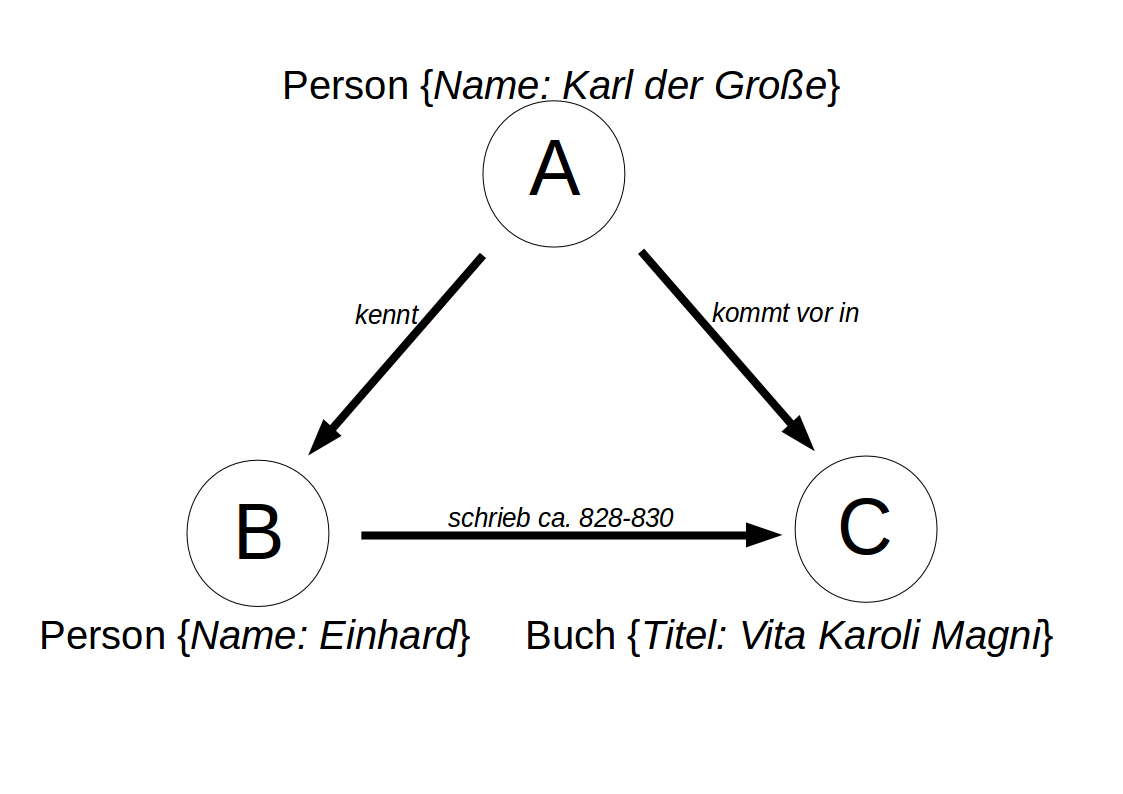
\includegraphics{Bilder/Beispielgraph.png}

Der zeigt oben einen Knoten (engl. Nodes) vom Typ Person mit der Eigenschaft Name. Diese hat den Wert ``Karl der Große''. Links unten ist ein weiter Knoten vom Typ Person mit dem Namen ``Einhard''. Rechts unten ist ein Knoten vom Typ Buch und dem Titel ``Vita Karoli Magni'' abgebildet. Die Kanten (engl. Edges) geben an, dass Karl der Große Einhart kannte, Einhard ca. 828-830 das Buch ``Vita Karoli Magni'' schrieb und Karl der Große in dem Buch vorkommt.

Knoten und Kanten können also noch zusätzliche Eigenschaften besitzen, in denen weitere Informationen gespeichert sind. Diese Eigenschaften sind spezifisch für die jeweiligen Knotentypen. So sieht man in der Abbildung, dass die beiden Knoten vom Typ Person jeweils noch die Eigenschaft Namen haben, deren Wert dann die Namen der Person angibt, während der Knoten vom Typ Buch die Eigenschaft Titel trägt, in dem der Titel des Buches abgespeichert wird.

\chapter{Installation und Start}\label{installation-und-start}

Informationen zur Installation von neo4j finden Sie auf den Dokumentationsseiten unter \url{https://neo4j.com/docs/operations-manual/current/installation/}. Für den normalen Nutzer empfiehlt sich die Installation von \href{https://neo4j.com/download/}{neo4j-Desktop}. Unter \url{https://neo4j.com/blog/this-week-in-neo4j-getting-started-with-neo4j-desktop-and-browser-graphileon-personal-edition-intuitive-detections-research-with-neo4j/?ref=twitter\#features-1} finden sich Videos, in denen die Installation von \href{https://www.youtube.com/watch?v=8yWhuUnPapw}{neo4j-Desktop} und erste Schritte im \href{https://www.youtube.com/watch?v=rQTximyaETA}{neo4j-Browser} erklärt werden.

\chapter{\texorpdfstring{Das Projekt Regesta Imperii oder ``Wie suchen Onlinenutzer Regesten''}{Das Projekt Regesta Imperii oder Wie suchen Onlinenutzer Regesten}}\label{das-projekt-regesta-imperii-oder-wie-suchen-onlinenutzer-regesten}

\section{Das Projekt Regesta Imperii}\label{das-projekt-regesta-imperii}

Das Projekt Regesta Imperii wurde von Johann-Friedrich Böhmer im Jahr 1829 begonnen. Ursprünglich als Vorarbeit zu den \href{https://www.mgh.de}{Monumenta Germaniae Historica} angelegt wurde es mit einem erweitereten Regestenkonzept bald zu einem unverzichtbaren Grundlagenwerk. In den Regesta Imperii werden Inhaltsangaben von Urkunden erstellt, die rechtlich relevante Personen, Inhalte, Orte und Sachverhalte in deutscher Sprache zusammenfassen. Zeitlich umfassen sie den Rahmen von den \href{https://de.wikipedia.org/wiki/Karolinger}{Karolingern} (7. Jahrhundert) bis Kaiser \href{https://de.wikipedia.org/wiki/Maximilian_I._(HRR)}{Maximilian} (gestorben 1519).

Beispielbild Urkunden

Ursprünglich von der DFG gefördert sind die Regesta Imperii heute Teil des Bund-Ländergeförderten Akademienprogramms und werden von der Akademie der Wissenschaften und der Literatur, Mainz, der Berlin-Brandenburgischen Akademie der Wissenschaften und der Akademie der Wissenschaften, Wien betreut.

Die Regesta Imperii arbeiten vor allem herrscherzentriert, d.h. in den Regesten muss der Herrscher eine zentrale Rolle spielen. Bei Urkundenregesten hat er selbst die Urkunde ausgestellt, bei historiographischen Regesten werden den Herrscher betreffende historische Hintergründe zusammengefasst.

\begin{figure}
\centering
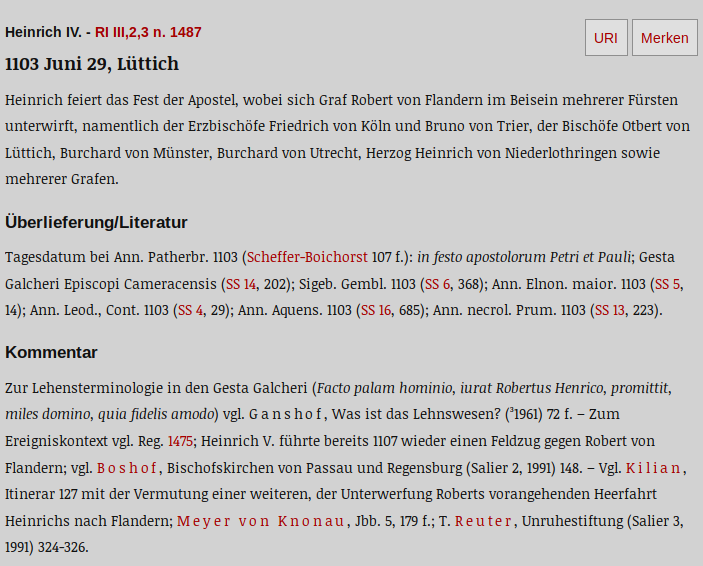
\includegraphics{Bilder/RI2Graph/ReggH4-Nr-1487.png}
\caption{RI III,2,3 n. 1487, in: Regesta Imperii Online, URI: http://www.regesta-imperii.de/id/cf75356b-bd0d-4a67-8aeb-3ae27d1dcefa.}
\end{figure}

In der Kopfzeile des Regests werden der Herrscher sowie Abteilung, Band und Regestennummer genannt. Die darunterliegende Datierungszeile nennt das Ausstellungsdatum der Urkunden und den Handlungs- bzw. Ausstellungsort. Es folgt der Regestentext mit der Zusammenfassung der Urkunde, Hinweise zur Originaldatierung, die Kanzleivermerke und schließlich Angaben zur Überlieferungssituation (Gibt es eine Originalurkunden, wo liegt sie, gibt es ggf. Abschriften etc.).

\section{Die Digitalisierung der Regesta Imperii}\label{die-digitalisierung-der-regesta-imperii}

Im Rahmen eines von der DFG geförderten Projekts wurden die Regesta Imperii gemeinsame von der Akademie der Wissenschaften, Mainz und der Bayrischen Staatsbibliothek München von 2001 bis 2006 komplett digitalisiert. Alle seit 2006 erschienenen Regesten wurden sofort im Volltext online gestellt. Glücklicherweise hatte die Mainzer Akademie die Rechte selbst inne, so dass der Veröffentlichung als Volltext im Internet keine rechtlichen Hürden im Wege standen. Rückblickend lässt sich feststellen, dass der Absatz der gedruckten Bände nicht gelitten sondern teilweise sogar etwas zugelegt hat.

\section{Wie suchen Online-Nutzer Regesten ?}\label{wie-suchen-online-nutzer-regesten}

Ende 2013 wurde das Suchverhalten der Nutzer der Online-Regestensuche im Rahmen eines Vortrages auf der Digital-Diplomatics-Konferenz in Paris in den Blick genommen.\footnote{Vgl. Kuczera, Andreas; Schrade, Torsten: From Charter Data to Charter Presentation: Thinking about Web Usability in the Regesta Imperii Online. Vortrag auf der Tagung ›Digital Diplomatikcs 2013 -- What ist Diplomatics in the Digital Environment?‹ Folien: https://prezi.com/vvacmdndthqg/from-charta-data-to-charta-presentation/.} Ein interessantes Ergebnis war die Häufigkeitsverteilung der Treffermengen pro Suchanfrage.

\begin{figure}
\centering
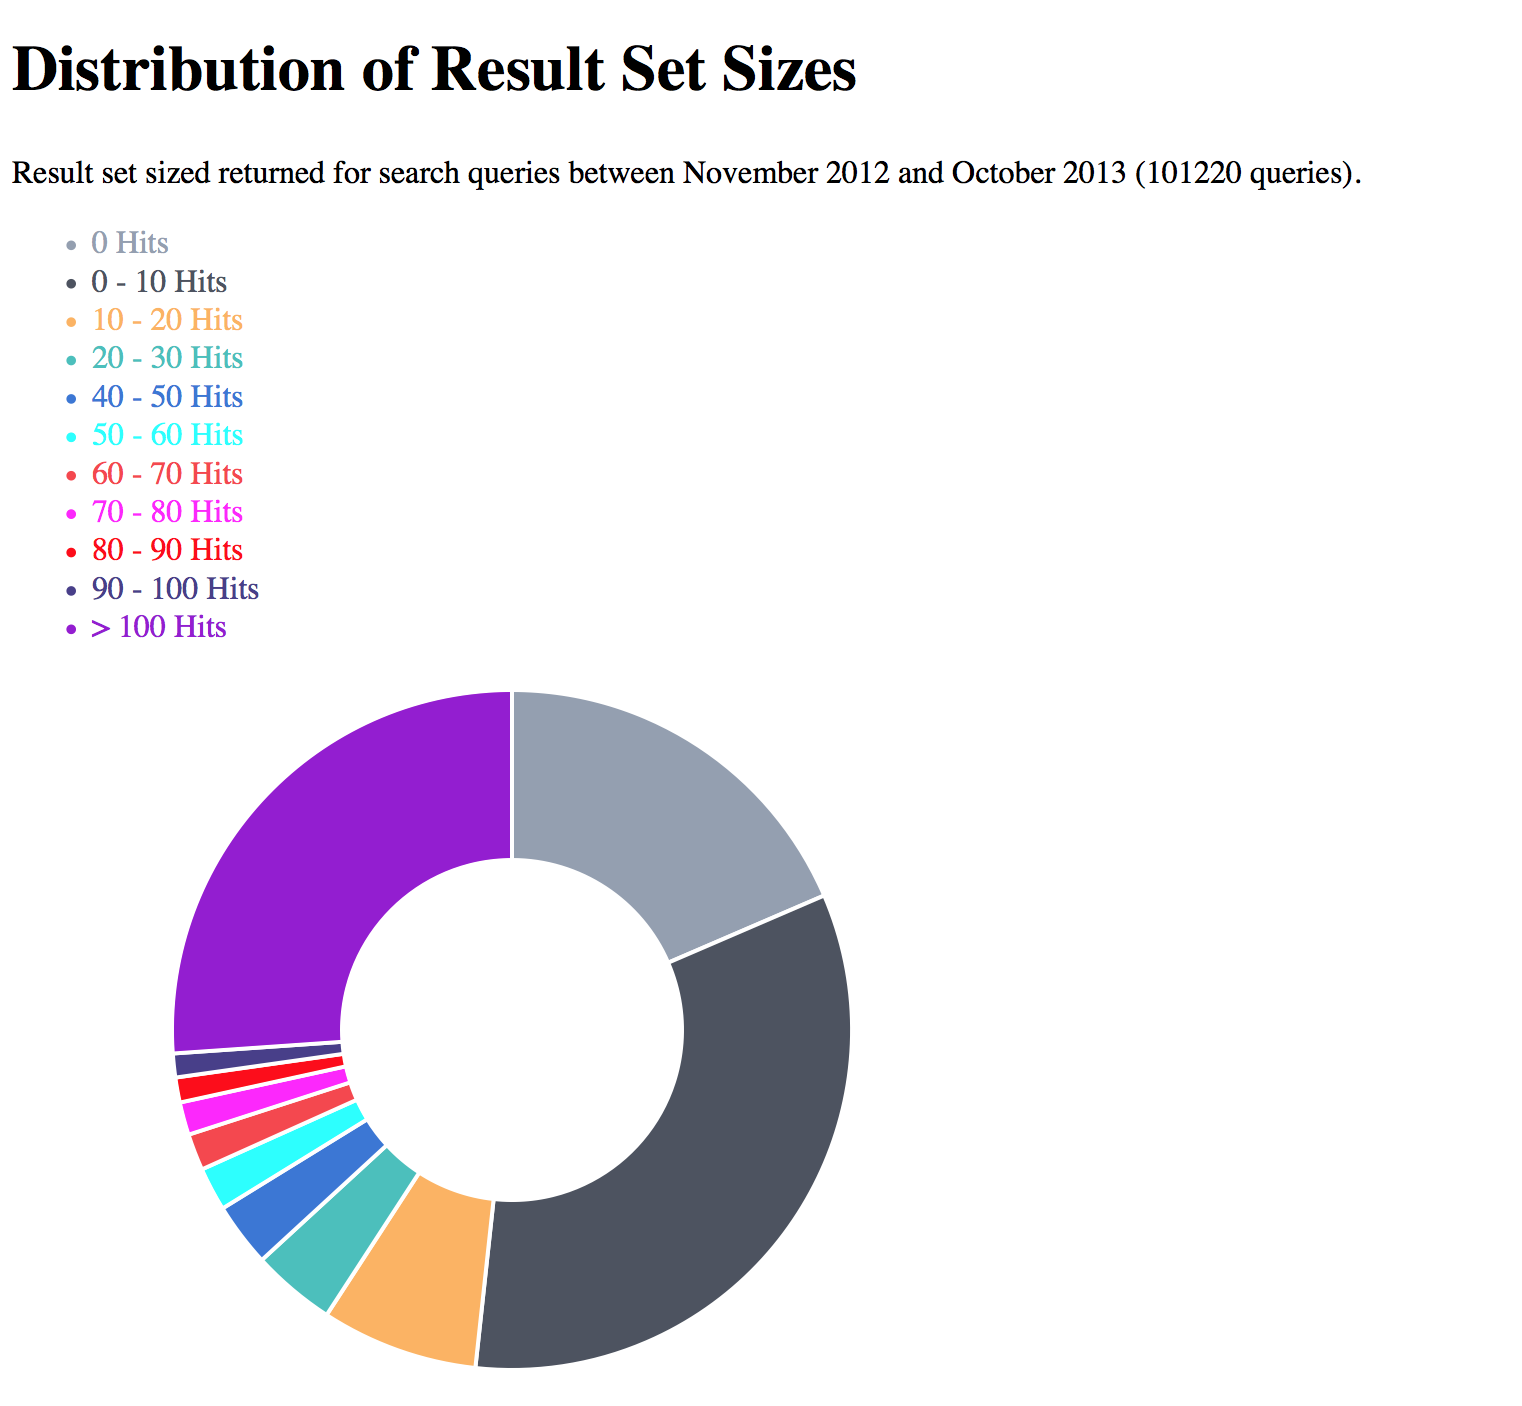
\includegraphics{Bilder/2012-Nutzungsformen_der_RI.png}
\caption{Treffermengen pro Suchanfragen im Jahr 2013.}
\end{figure}

Im Tortendiagramm ist die Treffermenge in Zehnerschritten angegeben. Die hellgraue Gruppe oben rechts hat keine Treffer, die dunkelgraue Gruppe einen bis zehn Treffer, die gelbe Gruppe 11 bis 20 usw. Die lila Gruppe hat mehr als hundert Treffer. Überraschend war die große Gruppe mit über 100 Treffern. Hinzu kam, dass über 68\% der Nutzer nur ein Suchwort in die Suchmaske eingegeben haben, wobei das beliebteste Suchwort \emph{Heinrich} Ende 2013 zu über 18.000 Treffern führte. Auf der Ergebnisseite hieß es dann: ``Sie suchten nach \emph{Heinrich}. Ihre Suche erzielte 18884 Treffer {[}\ldots{}{]} Sie sehen die Treffer 1 bis 20.''

Zusammenfassend könnte man feststellen, dass die Gruppe mit 1 bis 10 Treffern mit ihrem Ergebnis zufrieden war. 10 Regesten lassen sich gut ausdrucken und können anschließend gelesen, ausgewertet und in die eigene Forschungsarbeit einfließen. Die Gruppe mit keinem Treffer hatte möglicherweise die Suche zu sehr eingeschränkt oder einen Tippfehler beim Suchbegriff und wäre lieber in der Gruppe mit einem bis 10 Treffern. Selbstverständlich lassen sich auch 20 und mehr Treffer gut verarbeiten aber bei größeren Treffermengen steigt natürlich auch der Aufwand stark an, so dass davon auszugehen ist, dass die Nutzer kleinere, präzisere Ergebnisse bevorzugen.

Sehr gut lässt sich am Tortendiagramm auch ablesen, dass über die Hälfte unserer Nutzer vor der Suche eine genaue Vorstellung vom Ergebnis haben. Sie sind CIN-Nutzer (concrete information need). Die Gruppe mit über 100 Treffern können der Gruppe der POIN-Nutzer (problem-oriented information need) zugeordnet werden, die problemorientierte Anfragen haben. Für diese Nutzergruppe ist die aktuelle Trefferanzeige der Regestensuche unzureichend, da sie für ihre großen Treffermengen weitere Einschränkungsmöglichkeiten brauchen.\footnote{Näheres dazu in Kuczera, Andreas: Digitale Perspektiven mediävistischer Quellenrecherche, in: Mittelalter. Interdisziplinäre Forschung und Rezeptionsgeschichte, 18.04.2014. URL: mittelalter.hypotheses.org/3492.}

\section{Historische Netzwerkanalyse in den Registern}\label{historische-netzwerkanalyse-in-den-registern}

Im Bereich der historischen Netzwerkanalyse gab es in den letzten Jahren sehr interessante Arbeiten.\footnote{Vgl. beispielsweise Gramsch, Robert: Das Reich als Netzwerk der Fürsten - Politische Strukturen unter dem Doppelkönigtum Friedrichs II. und Heinrichs (VII.) 1225-1235. Ostfildern, 2013. Einen guten Überblick bietet das Handbuch Historische Netzwerkforschung - Grundlagen und Anwendungen. Herausgegeben von Marten Düring, Ulrich Eumann, Martin Stark und Linda von Keyserlingk. Berlin 2016.} von Seiten der Regesta Imperii bieten sich hier vor allem die Register der Regesta Imperi als sehr interessante Quelle an. Geht man davon aus, dass alle Personen, die gemeinsam in einem Regest genannt sind, etwas miteinander zu tun haben, könnte man auf Grundlage der Registerdaten ein Personennetzwerk erstellen. Über die Qualität der Beziehungen lässt sich nichts sagen und dies schränkt die Aussage der Daten ein. Andererseits stehen wiederum sehr viele Verknüpfungen zur Verfügung.

\begin{figure}
\centering
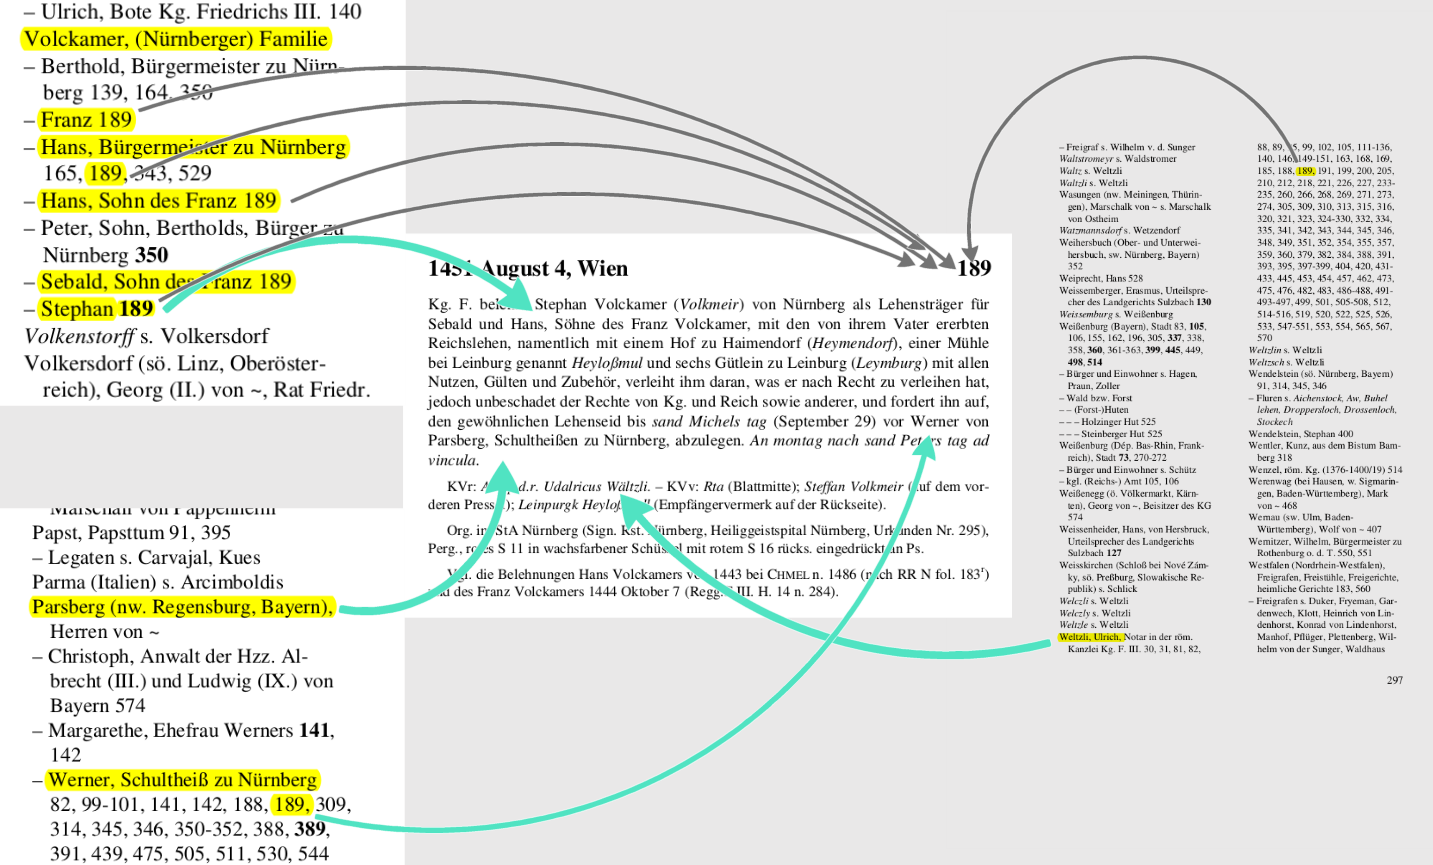
\includegraphics{Bilder/Register-und-Regest-19-189.png}
\caption{Registereinträge im Regest als Grundlage für ein Personennetzwerk.}
\end{figure}

Allein die Einträge in den Registern der Regesten Kaiser Friedrichs III. sind über 143.000 mal in Regesten genannt. Daraus ergeben sich dann über 460.000 1zu1-Beziehungen.\footnote{Der cypher-Befehl zur Erstellung der 1zu1-Beziehungen lautet: \emph{MATCH (n1:Registereintrag)-{[}:APPEARS\_IN{]}-\textgreater{}(r:Regest)\textless{}-{[}:APPEARS\_IN{]}-(n2:Registereintrag) MERGE (n1)-{[}:KNOWS{]}-\textgreater{}(n2);} Dabei werden die gerichteten \texttt{KNOWS}-Kanten jeweils in beide Richtungen erstellt. Mit folgendem Befehl lassen sich die \texttt{KNOWS}-Kanten zählen: \emph{MATCH p=()-{[}r:KNOWS{]}-\textgreater{}() RETURN count(p);} Für die Bestimmung der 1zu1-Beziehungen muss der Wert noch durch 2 geteilt werden.}

\begin{figure}
\centering
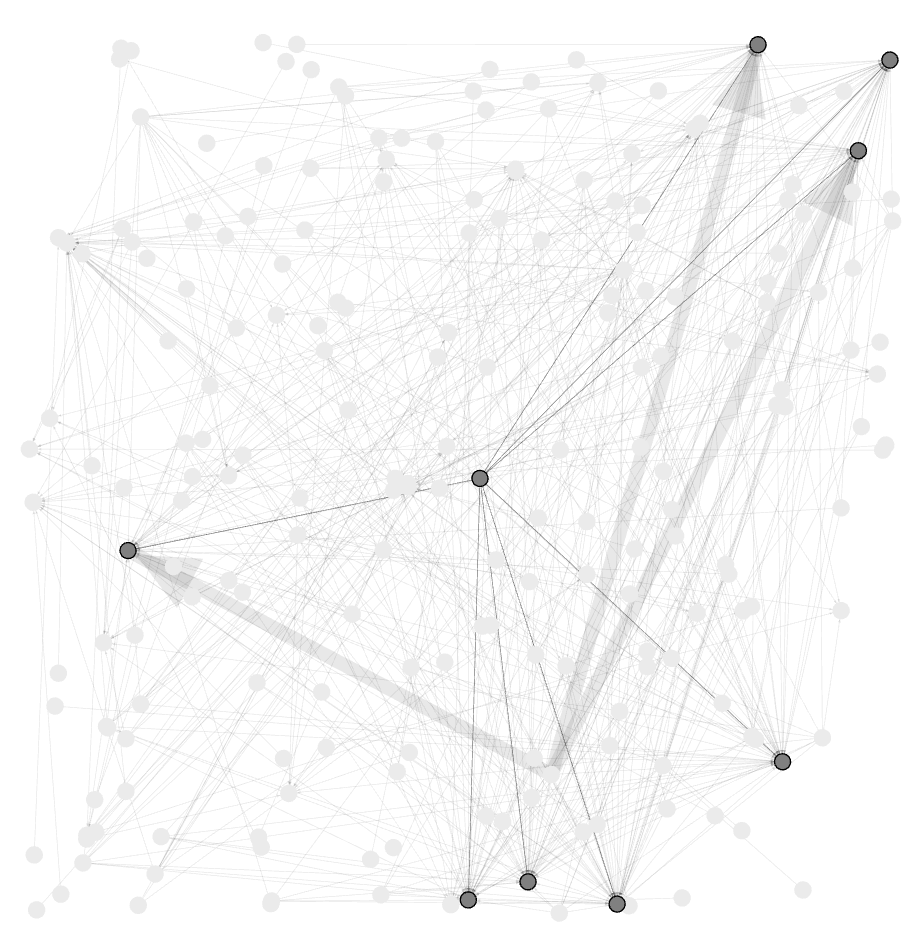
\includegraphics{Bilder/Gephi-Register.png}
\caption{Ausschnitt der 1zu1-Beziehungen in Gephi.}
\end{figure}

In der folgenden Abbildung sind die in den Registern des Regestenbandes von Joseph Chmel gewonnenen 1zu1-Beziehungen mit Gephi visualisiert.\footnote{Regesta chronologico-diplomatica Friderici III. Romanorum imperatoris (regis IV.) : Auszug aus den im K.K. Geheimen Haus-, Hof- und Staats-Archive zu Wien sich befindenden Registraturbüchern vom Jahre 1440 - 1493 ; nebst Auszügen aus Original-Urkunden, Manuscripten und Büchern / von Joseph Chmel, Wien 1838 und 1840.}

\begin{figure}
\centering
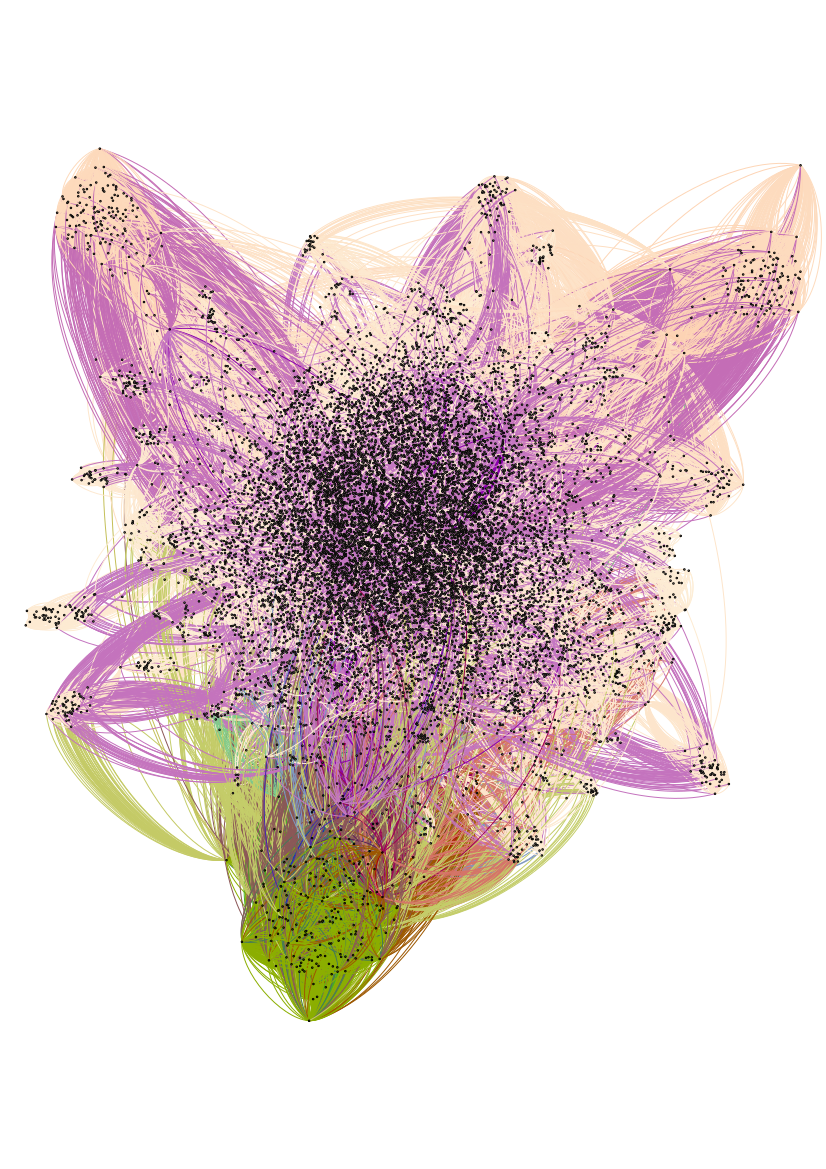
\includegraphics{Bilder/Chmelvisualisierung-v2.png}
\caption{Personennetzwerk aus den Registern der Regesten Chmels.}
\end{figure}

Bei der Analyse ergaben sich aber verschiedene Probleme. Zum einen werden in den Registern auch Kanzleibeamte genannt, die mit der eigentlichen Urkundenhandlung gar nichts zu tun hatten sondern später lediglich ihr Kürzel auf der Urkunde hinterließen. Dies mag archivgeschichtlich interessant sein, für die Urkundenhandlung ist es aber irrelevant. Ein zweites Problem ist der Aufbau des Registers, in dem Orte und Personen in einem Register zusammengefasst werden. Zum einen handelt es sich hierdurch nicht mehr um ein reines Personennetzwerk sondern um ein gemischtes Personen- und Ortsnetzwerk. Zum anderen überragen die über sehr lange Zeit bestehenden Orte, die in ihrer Lebensdauer begrenzten natürlichen Personen in den Netzwerkstrukturen. Schließlich zeigte sich, dass die Algrithmen zur Netzwerkanalyse mit zeitbehaftenen Daten (wie Regesten mit ihrem Ausstellungsdatum) nur schlecht umgehen konnten.

Aus Historikersicht war der Ansatz also weniger zielführend jedoch ergaben sich aus Modellierungssicht interessante Einblicke. Um die Netzwerke näher analysieren zu können, wurden kurze Zeitschnitte der Regesten untersucht. Hierfür musste das in Java geschriebene Programm zur Erstellung der Netzwerkdaten jedesmal umgeschrieben werden. Mein Kollege Ulli Meybohm, der das Programm damals betreute, wies mich nach dem wiederholten Umschreiben des Programms darauf hin, dass ich für meine Daten besser eine Graphdatenbank verwenden solle, beispielsweise neo4j. Erste Versuche des Imports der Registerdaten in neo4j erwiesen sich aber als sehr komplex, obwohl das Datenmodell \emph{Person kennt Person} eigentlich relativ einfach ist.

\begin{figure}
\centering
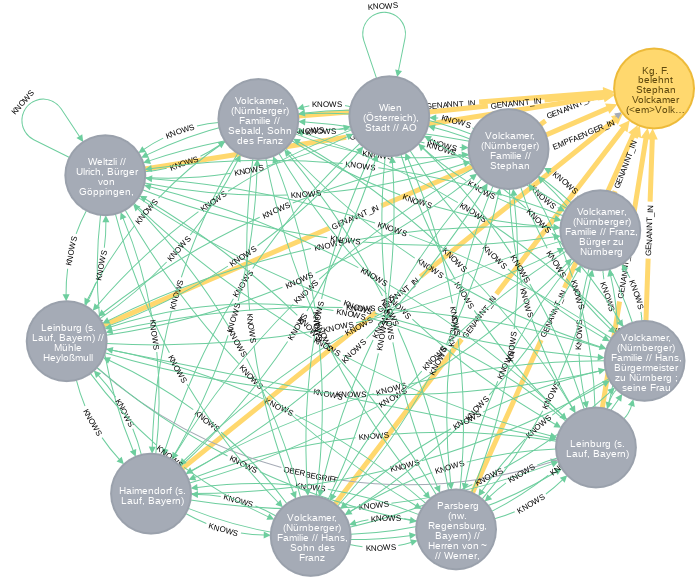
\includegraphics{Bilder/1zu1-Beziehungen-Register-Regest.png}
\caption{Regest und Registereinträge mit \texttt{GENANNT\_IN}-Kanten und den \texttt{KNOWS}-Kanten.}
\end{figure}

Schließlich ergaben Nachfragen bei neo4j, dass bei Problemen mit dem Datenmodell oft einfach ein Typ von Knoten vergessen worden sein könnte. Und tatsächlich wurden in den ersten Modellen die Regestenknoten nicht berücksichtigt. Mit den Regestenknoten im Modell war der Import schließlich mit weniger rechnerischem Aufwand möglich.

\begin{figure}
\centering
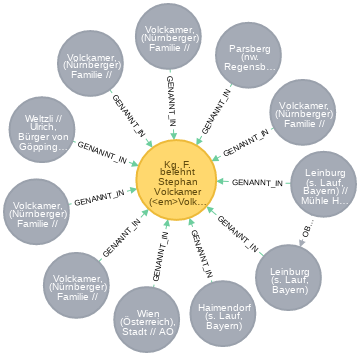
\includegraphics{Bilder/1zu1-Beziehungen-nur-Regest.png}
\caption{Graphmodell ohne \texttt{KNOWS}-Kanten. Diese können bei Bedarf einfach errechnet werden.}
\end{figure}

\section{Zusammenfassung}\label{zusammenfassung}

In diesem Kapitel wurde zunächst das Akademieprojekt Regesta Imperii vorgestellt. Seit der Anfang der 2000er Jahre erfolgten Digitalisierung stehen die Regesten unter \url{www.regesta-imperii.de} unter Creative-Commons-Lizenz frei im Internet zur Nutzung zur Verfügung. Für die Auswertung gibt es eine einfache Suchmaske und eine erweiterte Suche. Für die Jahre 2012 und 2013 wurde die Suchstrategien der Nutzer in der Online-Regestensuche untersucht und es zeigte sich, dass sich zwei Nutzungsszenarien unterscheiden lassen, von denen aber nur eines von den aktuellen Suchmasken der Regesta Imperii Online optimal bedient wird. Im zweiten Teil des Kapitels wurde die Visualisierung von Registernetzwerken und die anschließende Modellierung in Graphdatenbanken dargestellt und Nutzungs- und Auswertungsszenarien diskutiert. Im folgenden Kapitel wird die Modellierung von Regesten im Graphen detailliert erklärt.

\chapter{Regestenmodellierung im Graphen}\label{regestenmodellierung-im-graphen}

\section{Wie kommen die Regesten in den Graphen}\label{wie-kommen-die-regesten-in-den-graphen}

In diesem Abschnitt wird beispielhaft an Hand der Regesten Kaiser Heinrichs IV. der Import der Online-Regesten in die Graphdatenbank neo4j durchgespielt.\footnote{Die den Regesten Kaiser Heinrichs IV. umfassen folgende Bände: Böhmer, J. F., Regesta Imperii III. Salisches Haus 1024-1125. Tl. 2: 1056-1125. 3. Abt.: Die Regesten des Kaiserreichs unter Heinrich IV. 1056 (1050) - 1106. 1. Lief.: 1056 (1050) -- 1065, bearb. von Struve, Tilman - Köln (u.a.) (1984). Böhmer, J. F., Regesta Imperii III. Salisches Haus 1024-1125. Tl. 2: 1056-1125. 3. Abt.: Die Regesten des Kaiserreichs unter Heinrich IV. 1056 (1050) - 1106. 2. Lief.: 1065--1075, bearb. von Struve, Tilman unter Mitwirkung von Lubich, Gerhard und Jäckel, Dirk - Köln (u.a.) (2010). Böhmer, J. F., Regesta Imperii III. Salisches Haus 1024-1125. Tl. 2: 1056-1125. 3. Abt.: Die Regesten des Kaiserreichs unter Heinrich IV. 1056 (1050) - 1106. 3. Lief.: 1076--1085, bearb. von Lubich, Gerhard nach Vorarbeiten von Struve, Tilman unter Mitwirkung von Jäckel, Dirk - Köln (u.a.) (2016). Böhmer, J. F., Regesta Imperii III. Salisches Haus 1024-1125. Tl. 2: 1056-1125. 3. Abt.: Die Regesten des Kaiserreichs unter Heinrich IV. 1056 (1050) - 1106. 4. Lief.: 1086--1105/06, bearb. von Lubich, Gerhard nach Vorarbeiten von Brauch, Daniel unter Mitwirkung von Weber, Matthias - Köln (u.a.) (2016). Böhmer, J. F., Regesta Imperii III. Salisches Haus 1024-1125. Tl. 2: 1056-1125. 3. Abt.: Die Regesten des Kaiserreichs unter Heinrich IV. 1056 (1050) - 1106. 5. Lief.: Die Regesten Rudolfs von Rheinfelden, Hermanns von Salm und Konrads (III.). Verzeichnisse, Register, Addenda und Corrigenda, bearbeitet von Lubich, Gerhard unter Mitwirkung von Junker, Cathrin; Klocke, Lisa und Keller, Markus - Köln (u.a.) (2018).} Die Webseite der Regesta Imperii Online basiert auf dem Content-Managment-System typo3, welches auf eine mysql-Datenbank aufbaut. In der Datenbank werden die Regesteninformationen in verschiedenen Tabellen vorgehalten. Die Webseite bietet zum einen die Möglichkeit, die Regesten über eine REST-Schnittstelle im CEI-XML-Format oder als CSV-Dateien herunterzuladen. Für den Import in die Graphdatenbank bietet sich das CSV-Format an.

\begin{figure}
\centering
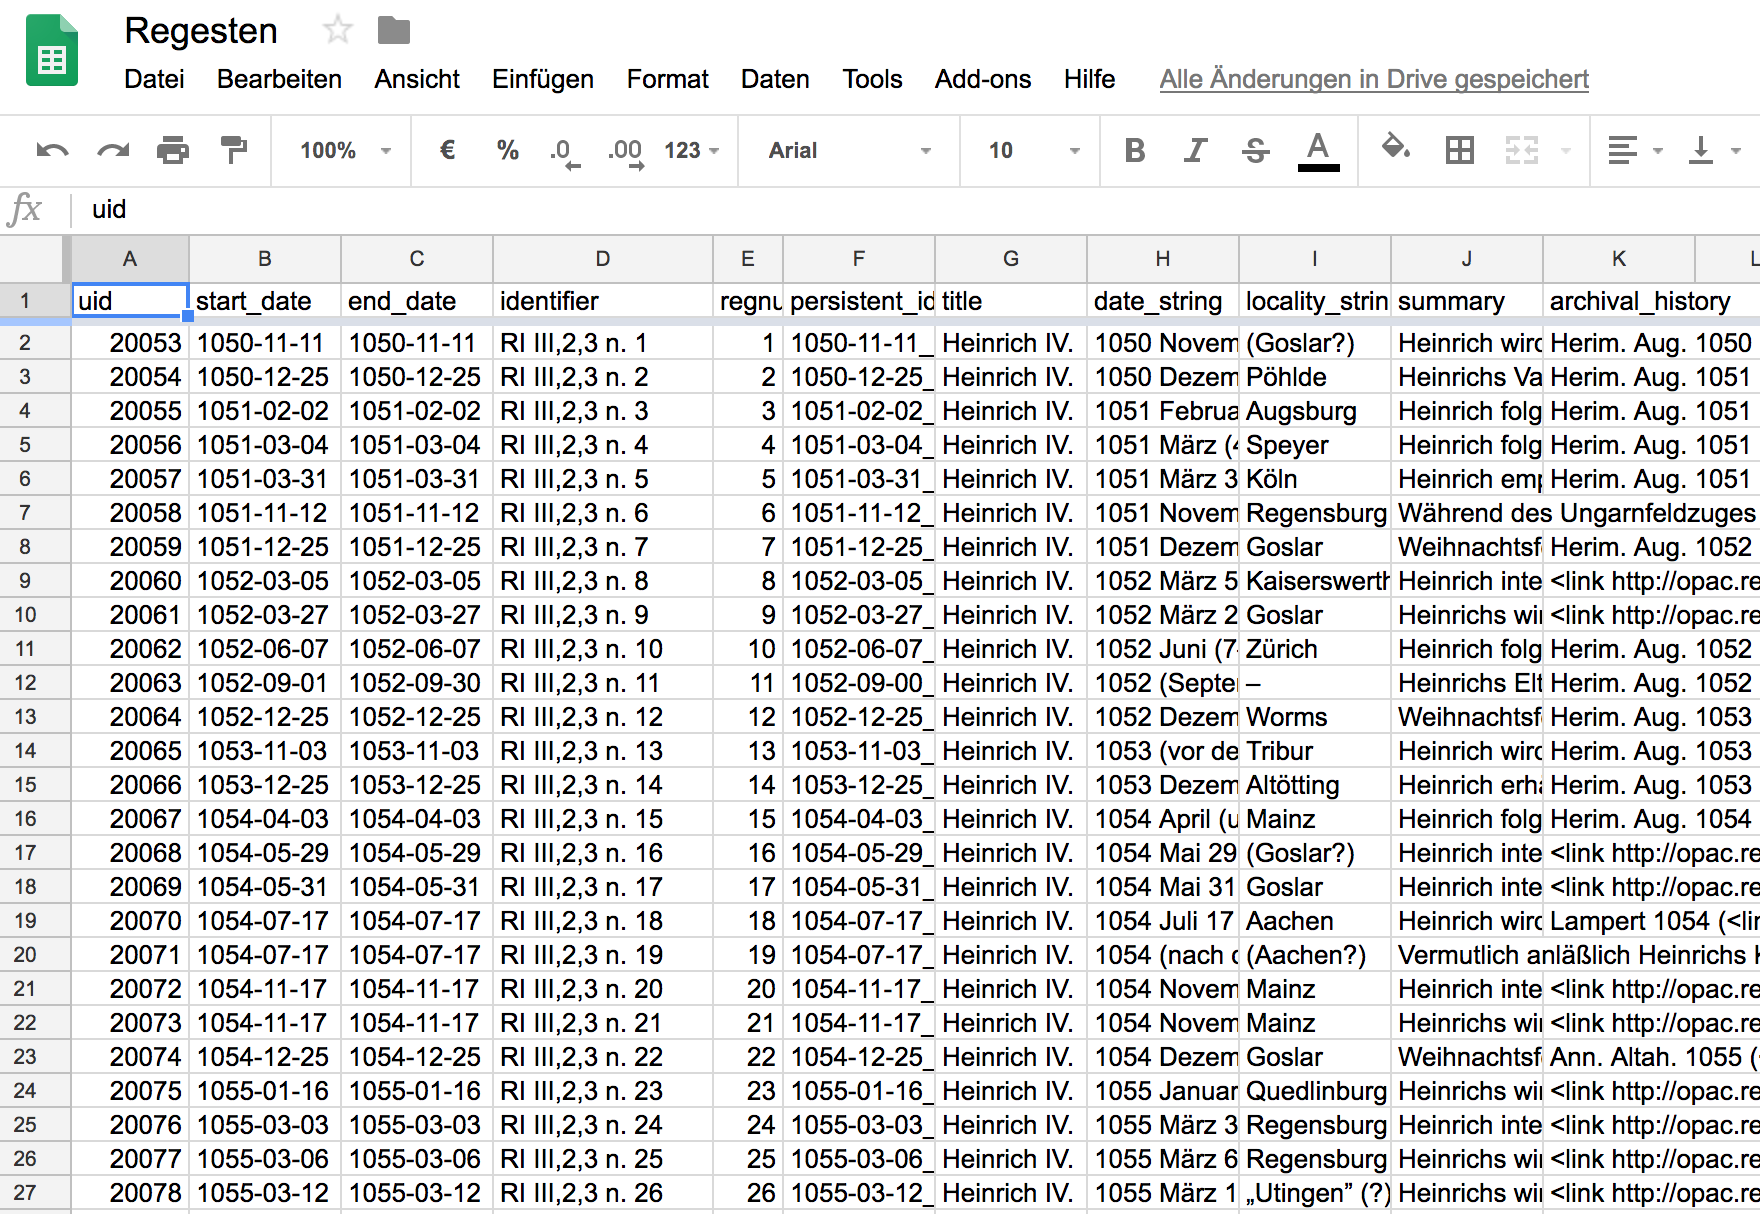
\includegraphics{Bilder/RI2Graph/ReggH4-Regestentabelle.png}
\caption{Regesten als CSV-Datei}
\end{figure}

In der CSV-Datei finden sich die oben erläuterten einzelnen Elemente der Regesten in jeweils eigenen Spalten. Die Spaltenüberschrift gibt Auskunft zum Inhalt der jeweiligen Spalte.

\subsection{\texorpdfstring{Import mit dem \texttt{LOAD\ CSV}-Befehl}{Import mit dem LOAD CSV-Befehl}}\label{import-mit-dem-load-csv-befehl}

Mit dem Befehl \texttt{LOAD\ CSV} können die CSV-Dateien mit den Regesten in die Graphdatenbank neo4j importiert werden.\footnote{Zu Installation und ersten Schritten von neo4j vgl. in der Einleitung den Abschnitt zu Installation und Start.} Hierfür muss die Datenbank aber Zugriff auf die CSV-Daten haben. Dies ist einerseits über den im Datenbankverzeichnis vorhandene Ordner \texttt{import} oder über eine URL, unter der die CSV-Datei abrufbar ist, möglich. Da sich die einzelnen Zugriffswege auf den \texttt{import}-Ordner von Betriebssystem zu Betriebssystem unterscheiden, wird hier beispielhaft der Import über eine URL vorgestellt. Hierfür wird ein Webserver benötigt, auf den man die CSV-Datei hochlädt und sich anschließend die Webadresse für den Download der Datei notiert.

\subsection{Google-Docs für den CSV-Download}\label{google-docs-fuxfcr-den-csv-download}

Es ist aber auch möglich, CSV-Daten in Google-spreadsheets zu speichern und dort eine URL für den Download der Daten zu erstellen. Zunächst benötigt man hierfür einen Google-Account. Anschließend öffnet man Google-Drive und erstellt dort eine leere Google-Tabellen-Datei (Google-Spreadsheet) in der man dann die CSV-Datei kopieren kann.

\begin{figure}
\centering
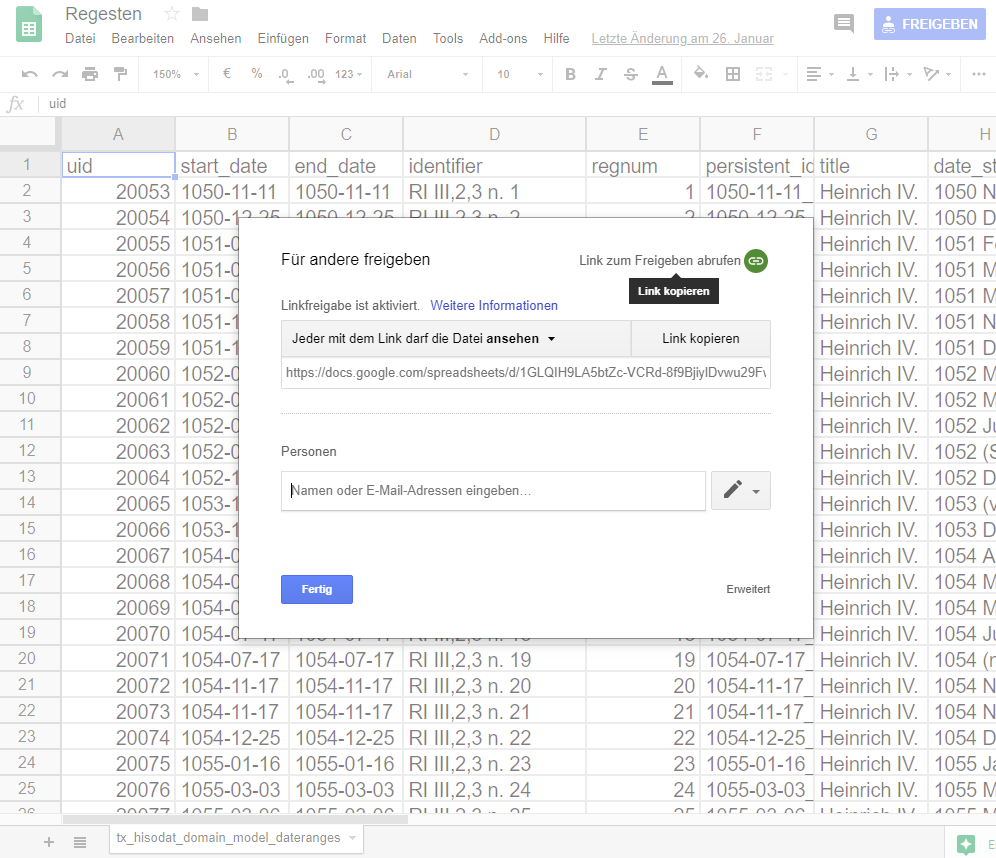
\includegraphics{Bilder/RI2Graph/google-docs-freigeben.png}
\caption{Freigabe der Datei zum Ansehen für Dritte!}
\end{figure}

Wichtig ist nun, die Datei zur Ansicht freizugeben (Klick auf \texttt{Freigeben} oben rechts im Fenster dann \texttt{Link\ zum\ Freigeben} abrufen und anschließend \texttt{Fertig} bestätigen). Jetzt ist die CSV-Datei in Google-Docs gespeichert und kann auch von anderen Personen über den Freigabelink angesehen werden. Für den Import in die Graphdatenbank benötigen wir aber einen Download im CSV-Format. Diesen findet man unter \texttt{Datei/Herunterladen\ als/Kommagetrennte\ Werte.csv\ aktuelles\ Tabellenblatt}.

\begin{figure}
\centering
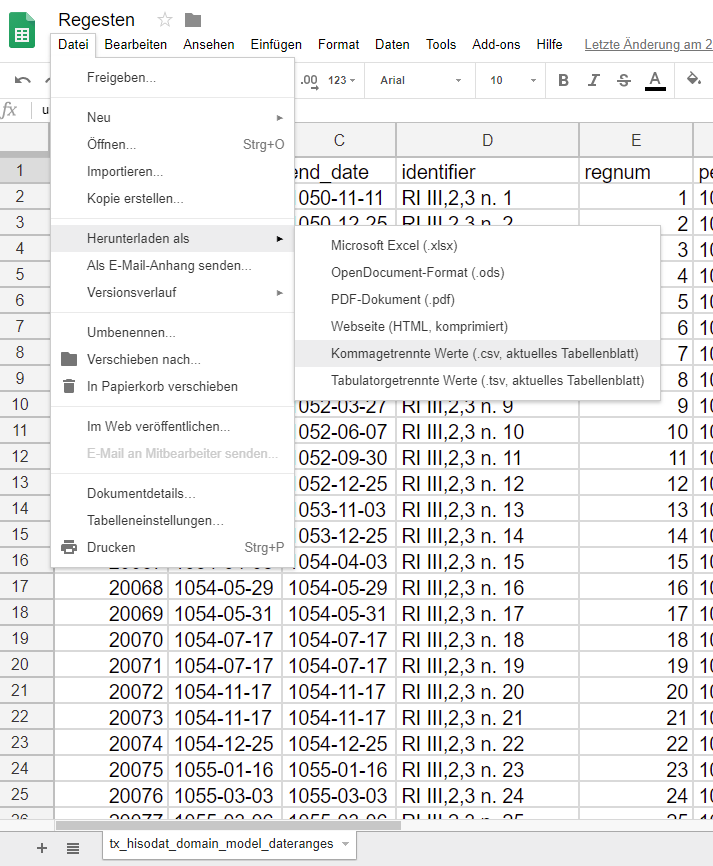
\includegraphics{Bilder/RI2Graph/google-docs-herunterladen-csv.png}
\caption{Herunterladen als CSV-DAtei}
\end{figure}

Damit erhält man das aktuelle Tabellenblatt als CSV-Download. Anschließend muss nun im Browser unter Downloads der Download-Link der Datei gesucht und kopiert werden.

\begin{figure}
\centering
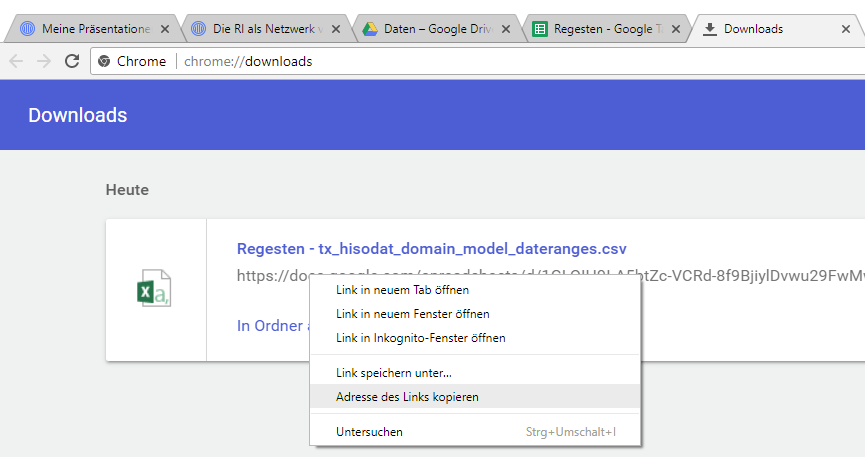
\includegraphics{Bilder/RI2Graph/google-docs-link-kopieren.png}
\caption{Download-Link der CSV-Datei}
\end{figure}

\subsection{Regestenmodellierung im Graphen}\label{regestenmodellierung-im-graphen-1}

Mit dem \texttt{LOAD\ CSV}-Befehl stehen die Informationen der Regestentabelle nun für die weitere Verarbeitung zur Verfügung. Nun muss festgelegt werden, wie diese Informationen im Graphen modelliert werden sollen. Daher wird im nächsten Schritt das Modell der Regesten im Graphen vorgestellt (siehe Abbildung).

\begin{figure}
\centering
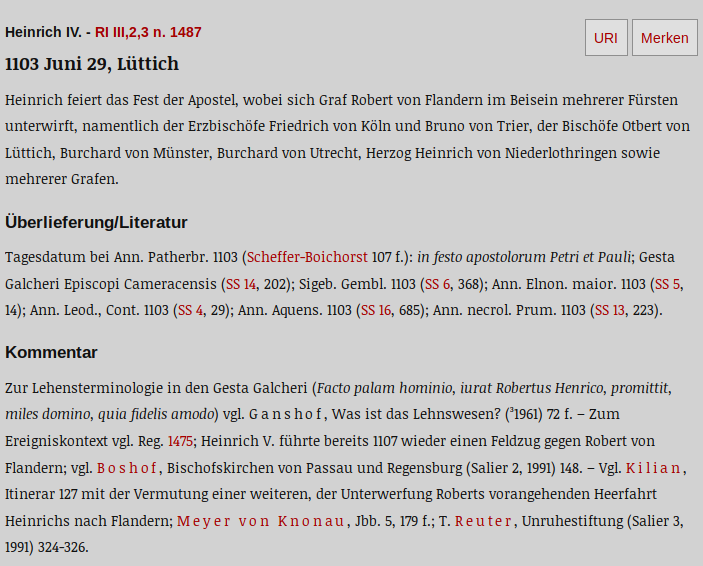
\includegraphics{Bilder/RI2Graph/ReggH4-Nr-1487.png}
\caption{RI III,2,3 n. 1487, in: Regesta Imperii Online, URI: http://www.regesta-imperii.de/id/cf75356b-bd0d-4a67-8aeb-3ae27d1dcefa.}
\end{figure}

\begin{figure}
\centering
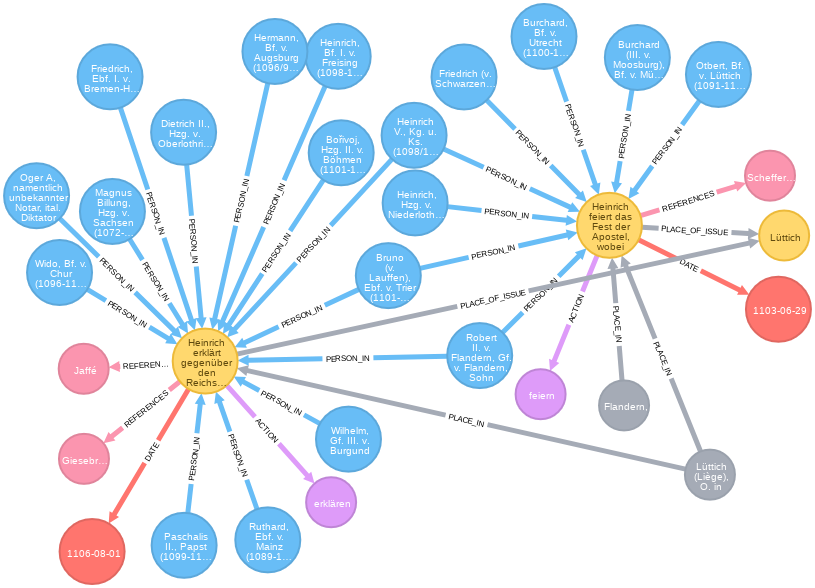
\includegraphics{Bilder/RI2Graph/ReggH4-Nr-1487imGraph.png}
\caption{Das Regest im Graphen.}
\end{figure}

In den Abbildungen finden sich beispielhaft das Regest RI III,2,3 Nr. 1487, einmal in der Ansicht der Onlineregesten und in der zweiten Abbildung als Modell im Graphen (neben anderen Regesten).

Die gelben Knoten sind die Regesten. Aus den Angaben des Regests werden mit dem o.a. Befehl noch ein Datumsknoten und ein Ortsknoten erstellt. Mit dem ersten \texttt{CREATE}-Befehl werden die Regesten erstellt. Die \texttt{MERGE}-Befehle erzeugen ergänzende Knoten für die Datumsangaben und die Ausstellungsorte. Nun ist es aber so, dass Ausstellungsort und Ausstellungsdatum mehrfach vorkommen können. Daher wird hier nicht der \texttt{CREATE}-Befehl sondern der \texttt{MERGE}-Befehl verwendet. Dieser funktioniert wie der \texttt{CREATE}-Befehl, prüft aber vorher, ob in der Datenbank ein solcher Knoten schon existiert. Falls es ihn noch nicht gibt, wird er erzeugt, wenn es ihn schon gibt, wird er der entsprechenden Variable zugeordnet. Anschließend wird die Kante zwischen Regestenknoten und Ausstellungsortsknoten und Regestenknoten und Datumsknoten erstellt. In der folgenden Tabelle werden die einzelnen Befehle dargestellt und kommentiert.

\subsection{Indexe Erstellen}\label{indexe-erstellen}

Bevor nun mit dem Import begonnen wird, ist es für die Beschleunigung des Importprozesses von Vorteil vorher Indexe für häufig genutzte Properties zu erstellen.

\begin{verbatim}
// vorab Index erzeugen -> Import wird schneller
CREATE INDEX ON :Regesta(ident);
CREATE INDEX ON :Regesta(regnum);
CREATE INDEX ON :Regesta(persistentIdentifier);
CREATE INDEX ON :Regesta(registerId);
CREATE INDEX ON :Regesta(heftId);
CREATE INDEX ON :Regesta(placeOfIssue);
CREATE INDEX ON :Regesta(origPlaceOfIssue);
CREATE INDEX ON :Date(startDate);
CREATE INDEX ON :Place(original);
CREATE INDEX ON :Place(normalizedGerman);
CREATE INDEX ON :Lemma(lemma);
CREATE INDEX ON :Literature(literatur);
CREATE INDEX ON :Reference(reference);
CREATE INDEX ON :IndexEntry(registerId);
CREATE INDEX ON :IndexEntry(nodeId);
CREATE INDEX ON :Regesta(latLong);
CREATE INDEX ON :IndexPlace(registerId);
CREATE INDEX ON :IndexEvent(registerId);
CREATE INDEX ON :IndexPerson(registerId);
\end{verbatim}

\subsection{Erstellen der Regestenknoten}\label{erstellen-der-regestenknoten}

Mit dem folgenden cypher-Query werden die Regestenknoten in der Graphdatenbank erstellt:

\begin{verbatim}
// Regestenknoten erstellen
LOAD CSV WITH HEADERS FROM "https://docs.google.com/spreadsheets/d/
1GLQIH9LA5btZc-VCRd-8f9BjiylDvwu29FwMwksBbrE/
export?format=csv&id=1GLQIH9LA5btZc-VCRd-
8f9BjiylDvwu29FwMwksBbrE&gid=2138530170" AS line
CREATE (r:Regesta {regid:line.persistentIdentifier, text:line.summary,
  archivalHistory:line.archival_history, date:line.date_string,  
  ident:line.identifier,  regnum:line.regnum,
  origPlaceOfIssue:line.locality_string, startDate:line.start_date,
  endDate:line.end_date})
MERGE (d:Date {startDate:line.start_date, endate:line.end_date})
MERGE (r)-[:DATE]->(d)
RETURN count(r);
\end{verbatim}

Im folgenden werden die einzelnen Teile des Import-Befehls erläutert:

\begin{longtable}[]{@{}lll@{}}
\toprule
\begin{minipage}[b]{0.31\columnwidth}\raggedright\strut
Befehl\strut
\end{minipage} & \begin{minipage}[b]{0.23\columnwidth}\raggedright\strut
Variablen\strut
\end{minipage} & \begin{minipage}[b]{0.37\columnwidth}\raggedright\strut
Bemerkungen\strut
\end{minipage}\tabularnewline
\midrule
\endhead
\begin{minipage}[t]{0.31\columnwidth}\raggedright\strut
\texttt{LOAD\ CSV\ WITH\ HEADERS\ FROM} ``https://docs.google.com/ \ldots{}'' AS line\strut
\end{minipage} & \begin{minipage}[t]{0.23\columnwidth}\raggedright\strut
line\strut
\end{minipage} & \begin{minipage}[t]{0.37\columnwidth}\raggedright\strut
Import der CSV-Dateien. Es wird jeweils eine Zeile an die Variable line weitergegeben\strut
\end{minipage}\tabularnewline
\begin{minipage}[t]{0.31\columnwidth}\raggedright\strut
\texttt{CREATE}(r:Regesta \{regid:line.persistentIdentifier, text:line.summary, archivalHistory:line.archival\_history, date:line.date\_string\strut
\end{minipage} & \begin{minipage}[t]{0.23\columnwidth}\raggedright\strut
line.persistent\_ identifier, line.summary etc.\strut
\end{minipage} & \begin{minipage}[t]{0.37\columnwidth}\raggedright\strut
Erstellung des Regestenknotens. Für die weiteren Befehle steht der neu erstellt Regestenknoten unter der Variable \texttt{r} zur Verfügung.\strut
\end{minipage}\tabularnewline
\begin{minipage}[t]{0.31\columnwidth}\raggedright\strut
\texttt{MERGE} (d:Date \{startDate:line.start\_date, endate:line.end\_date\})\strut
\end{minipage} & \begin{minipage}[t]{0.23\columnwidth}\raggedright\strut
line.start\_date und line.end\_date\strut
\end{minipage} & \begin{minipage}[t]{0.37\columnwidth}\raggedright\strut
Es wird geprüft, ob ein Datumsknoten mit der Datumsangabe schon existiert, falls nicht, wird er erstellt. In jedem Fall steht anschließend der Datumsknoten unter der Variable d zur Verfügung.\strut
\end{minipage}\tabularnewline
\begin{minipage}[t]{0.31\columnwidth}\raggedright\strut
\texttt{MERGE} (r)-{[}:HAT\_DATUM{]}-\textgreater{}(d)\strut
\end{minipage} & \begin{minipage}[t]{0.23\columnwidth}\raggedright\strut
\texttt{(r)} ist der Regestenknoten, \texttt{(d)} ist der Datumsknoten\strut
\end{minipage} & \begin{minipage}[t]{0.37\columnwidth}\raggedright\strut
Zwischen Regestenknoten und Datumsknoten wird eine \texttt{HAT\_DATUM}-Kante erstellt.\strut
\end{minipage}\tabularnewline
\bottomrule
\end{longtable}

\subsection{Erstellen der Ausstellungsorte}\label{erstellen-der-ausstellungsorte}

In den Kopfzeilen der Regesten ist, soweit bekannt, der Ausstellungsort der Urkunde vermerkt. Im Rahmen der Arbeiten an den Regesta Imperii Online wurden diese Angaben zusammengestellt und soweit möglich die Orte identifiziert, so dass diese Angabe nun beim Import der Regesten in den Graphen berücksichtigt werden kann. Insgesamt befinden sich in den Regesta Imperii über 12.000 verschiedene Angaben für Ausstellungsorte, wobei sie sich aber auch teilweise auf den gleichen Ort beziehen können (Wie z.B. Aachen, Aquisgrani, Aquisgradi, Aquisgranum, coram Aquisgrano etc.). Allein mit der Identifizierung der 1.000 häufigsten Ortsangaben konnte schon die überwiegende Mehrzahl der Ausstellungsorte georeferenziert werden. Die Daten zur Ortsidentifizierung liegen auch in einer Google-Tabelle vor.

Mit dem folgenden cypher-Query werden die Ausstellungsorte in die Graphdatenbank importiert:

\begin{verbatim}
// RI-Ausstellungsorte-geo erstellen
LOAD CSV WITH HEADERS FROM "https://docs.google.com/spreadsheets/d/
13_f6Vja4HfOpju9RVDubHiMLzS6Uoa7MIOHFEg5V7lw/
export?format=csv&id=13_f6Vja4HfOpju9RVDubHiMLzS6Uoa7MIOHFEg5V7lw
&gid=420547059"
AS line
WITH line
WHERE line.Lat IS NOT NULL
AND line.normalisiertDeutsch IS NOT NULL
MATCH (r:Regesta {origPlaceOfIssue:line.Original})
MERGE (p:Place {normalizedGerman:line.normalisiertDeutsch,
  longitude:line.Long, latitude:line.Lat})
WITH r, p, line
MERGE (r)-[rel:PLACE_OF_ISSUE]->(p)
SET p.wikidataId = line.wikidataId
SET p.name = line.name
SET p.gettyId = line.GettyId
SET p.geonamesId = line.GeonamesId
SET rel.original = line.Original
SET rel.alternativeName = line.Alternativname
SET rel.commentary = line.Kommentar
SET rel.allocation = line.Zuordnung
SET rel.state = line.Lage
SET rel.certainty = line.Sicherheit
SET rel.institutionInCity = line.InstInDerStadt
RETURN count(p);
\end{verbatim}

Da Import-Query etwas komplexer ist, wird er im folgenden näher erläutert. Nach dem \texttt{LOAD\ CSV\ WITH\ HEADERS\ FROM}-Befehl wird zunächst überprüft, ob der jeweils eingelesene Eintrag in der Spalte \texttt{line.lat} und in der Spalte \texttt{line.normalisiertDeutsch} Einträge hat. Ist dies der Fall wird überprüft, ob es einen Regestenknoten gibt, der einen Ausstellungsorteintrag hat, der der Angabe in der Spalte \texttt{Original} entspricht. Diese Auswahl ist notwendig, da in der Tabelle die Ausstellungsorte der gesamten Regesta Imperii enthalten sind. Für diesen Import sollen aber nur jene angelegt werden, die für die Regesten Kaiser Heinrichs IV. relevant sind. Mit dem \texttt{MERGE}-Befehl wird der \texttt{Place}-Knoten erstellt (falls es ihn nicht schon gibt) und anschließend mit dem Regestenknoten verknüpft. Schließlich werden noch weitere Details der Ortsangabe im \texttt{Place}-Knoten und in den \texttt{PLACE\_OF\_ISSUE}-Kanten ergänzt.

\subsection{Koordinaten der Ausstellungsorte}\label{koordinaten-der-ausstellungsorte}

Mit dem folgenden Query werden die Koordinatenangaben zu Höhen- und Breitengraden der Ausstellungsorte (\texttt{Place}-Knoten), die in den Propertys latitude und longitude abgespeichert sind, in der neuen Property LatLong zusammengefasst und in \texttt{point}-Werte umgewandelt. Seit Version 3 kann neo4j mit diesen Werten Abstandsberechnungen durchführen (Mehr dazu siehe unten bei den Auswertungen).

\begin{verbatim}
// Regesten und Ausstellungsorte mit Koordinaten der Ausstellungsorte versehen
MATCH (r:Regesta)-[:PLACE_OF_ISSUE]->(o:Place)
SET r.latLong = point({latitude: tofloat(o.latitude),
  longitude: tofloat(o.longitude)})
SET o.latLong = point({latitude: tofloat(o.latitude),
  longitude: tofloat(o.longitude)})
SET r.placeOfIssue = o.normalizedGerman
SET r.latitude = o.latitude
SET r.longitude = o.longitude;
\end{verbatim}

\subsection{Ausstellungsdatum}\label{ausstellungsdatum}

In den Regesta Imperii Online sind die Datumsangaben der Regesten iso-konform im Format JJJJ-MM-TT (also Jahr-Monat-Tag) abgespeichert. neo4j behandelt diese Angaben aber als String. Um Datumsberechnungen durchführen zu können, müssen die Strings in neo4j-interne Datumswerte umgerechnet werden. Der cypher-Query hierzu sieht wie folgt aus:

\begin{verbatim}
// Date in neo4j-Datumsformat umwandeln
MATCH (n:Regesta)
SET n.isoStartDate = date(n.startDate);
MATCH (n:Regesta)
SET n.isoEndDate = date(n.endDate);
MATCH (d:Date)
SET d.isoStartDate = date(d.startDate);
MATCH (d:Date)
SET d.isoEndDate = date(d.endDate);
\end{verbatim}

Zunächst werden mit dem \texttt{MATCH}-Befehl alle Regestenknoten aufgerufen. Anschließend wird für jeden Regestenknoten aus der String-Property \texttt{startDate} die Datumsproperty \texttt{isoStartDate} berechnet und im Regestenknoten abgespeichert. Mit Hilfe der Property können dann Datumsangaben und Zeiträume abgefragt werden (Beispiel hierzu unten in der Auswertung).

\section{Exkurs: Herrscherhandeln in den Regesta Imperii}\label{exkurs-herrscherhandeln-in-den-regesta-imperii}

Bisher wurden beim Import der Regesten in den Graphen nur die in den Online-Regesten bereits angelegten Angaben importiert. Im folgenden Schritt werden nun in einem kleinen Exkurs die Regestentexte selbst analysiert und anschließend die Graphdatenbank um eine weitere Informationsebene ergänzt. Regesten sind in ihrer Struktur stark formalisiert. Meist wird mit dem ersten Verb im Regest das Herrscherhandeln beschrieben. Um dies auch digital auswerten zu können, haben wir in einem kleinen Testprojekt mit Hilfe des \href{http://www.cis.uni-muenchen.de/~schmid/tools/TreeTagger/}{Stuttgart-München Treetaggers}\footnote{Zum Treetagger vgl. http://www.cis.uni-muenchen.de/\textasciitilde{}schmid/tools/TreeTagger/.} aus jedem Regest das erste Verb extrahiert und normalisiert. Die Ergebnisse sind in folgender \href{https://docs.google.com/spreadsheets/d/1nlbZmQYcT1E3Z58yPmcnulcNQc1e3111Di-4huhV-FY/edit?usp=sharing}{Tabelle} einsehbar. Diese Tabelle wird mit dem folgenden cypher-Query in die Graphdatenbank eingelesen.

\begin{verbatim}
// ReggH4-Herrscherhandeln
LOAD CSV WITH HEADERS FROM "https://docs.google.com/spreadsheets/d/1nlbZmQYcT1E3Z58yPmcnulcNQc1e3111Di-4huhV-FY/export?format=csv&id=1nlbZmQYcT1E3Z58yPmcnulcNQc1e3111Di-4huhV-FY&gid=267441060"
AS line FIELDTERMINATOR ','
MATCH (r:Regesta{ident:line.regid})
MERGE (l:Lemma{lemma:line.Lemma})
MERGE (r)-[:ACTION]->(l);
\end{verbatim}

Dabei wird zunächst mit dem \texttt{MATCH}-Befehl das jeweilige Regest gesucht, anschließend mit dem \texttt{MERGE}-Befehl der \texttt{Lemma}-Knoten für das Herrscherhandeln angelegt (falls noch nicht vorhanden) und schließlich der \texttt{Regesta}-knoten mit dem \texttt{Lemma}-Knoten über eine \texttt{ACTION}-Kante verbunden. In der folgenden Abbildung ist ein Ausschnitt mit Regesten und den verknüpften Lemmaknoten dargestellt.

\begin{figure}
\centering
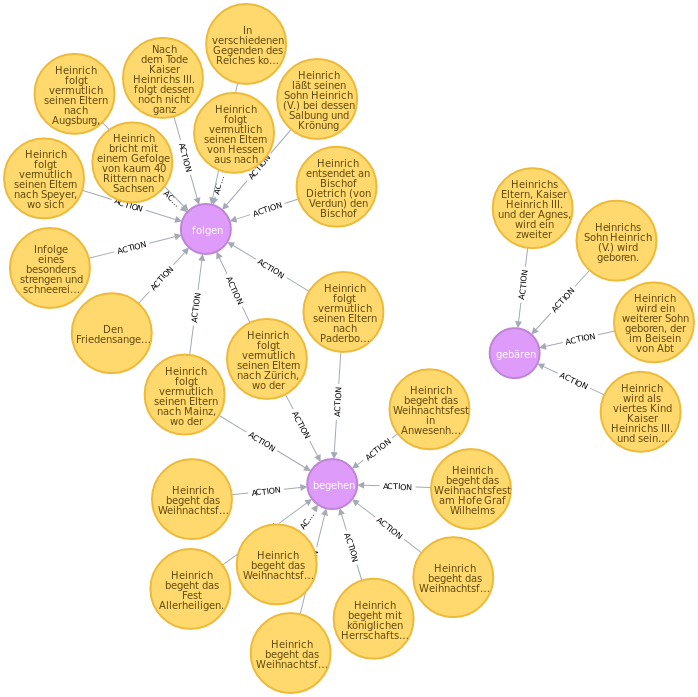
\includegraphics{Bilder/RI2Graph/ReggH4-Action.png}
\caption{Herrscherhandeln im Graphen.}
\end{figure}

\section{Zitationsnetzwerke in den Regesta Imperii}\label{zitationsnetzwerke-in-den-regesta-imperii}

In vielen Online-Regesten ist die zitierte Literatur mit dem \href{http://opac.regesta-imperii.de/lang_de/}{Regesta-Imperii-Opac} verlinkt. Da es sich um URLs handelt, sind diese Verweise eindeutig. Andererseits lassen sie sich mit regulären Ausdrücken aus den Regesten extrahieren. Mit folgendem Query werden aus den Überlieferungsteilen der Regesten die mit dem Opac verlinkten Literaturangaben extrahiert und jede Literaturangabe als \texttt{Refernce}-Knoten angelegt.

\begin{verbatim}
// ReggH4-Literaturnetzwerk erstellen
MATCH (reg:Regesta)
WHERE reg.archivalHistory CONTAINS "link"
UNWIND apoc.text.regexGroups(reg.archivalHistory,
"<link (\\S+)>(\\S+)</link>") as link
MERGE (ref:Reference {url:link[1]})
ON CREATE SET ref.title=link[2]
MERGE (reg)-[:REFERENCES]->(ref);
\end{verbatim}

Da dies mit dem \texttt{MERGE}-Befehl geschieht, wird in der Graphdatenbank jeder Literaturtitel nur einmal angelegt. Anschließend werden die \texttt{Reference}-Knoten mit den Regesten über \texttt{REFERNCES}-Kanten verbunden. Zu den Auswertungsmöglichkeiten vgl. unten den Abschnitt zu den \protect\hyperlink{ux5cux23Auswertungsperspektiven}{Auswertungsperspektiven}.

\section{Import der Registerdaten in die Graphdatenbank}\label{import-der-registerdaten-in-die-graphdatenbank}

\subsection{Vorbereitung der Registerdaten}\label{vorbereitung-der-registerdaten}

Register spielen für die Erschließung von gedrucktem Wissen eine zentrale Rolle, da dort in alphabetischer Ordnung die im Werk vorkommenden Entitäten (z.B. Personen und Orte) hierarchisch gegliedert aufgeschlüsselt werden. Für die digitale Erschließung der Regesta Imperii sind Register von zentraler Bedeutung, da mit ihnen die in den Regesten vorkommenden Personen und Orte bereits identifiziert vorliegen. Für den Import in die Graphdatenbank wird allerdings eine digitalisierterte Fassung des Registers benötigt. Im Digitalisierungsprojekt Regesta Imperii Online wurden Anfang der 2000er Jahre auch die gedruckt vorliegenden Register digitalisiert. Sie dienen nun als Grundlage für die digitale Registererschließung der Regesta Imperii. Im hier gezeigten Beispiel werden die Regesten Kaiser Heinrichs IV. und das dazugehörige Register importiert. Da der letzte Regestenband der Regesten Kaiser Heinrichs IV. mit dem Gesamtregister erst vor kurzem gedruckt wurde, liegen hier aktuelle digitale Fassung von Registern und Regesten vor. Die für den Druck in Word erstellte Registerfassung wird hierfür zunächst in eine hierarchisch gegliederte XML-Fassung konvertiert, damit die Registerhierarchie auch maschinenlesbar abgelegt ist.

\begin{figure}
\centering
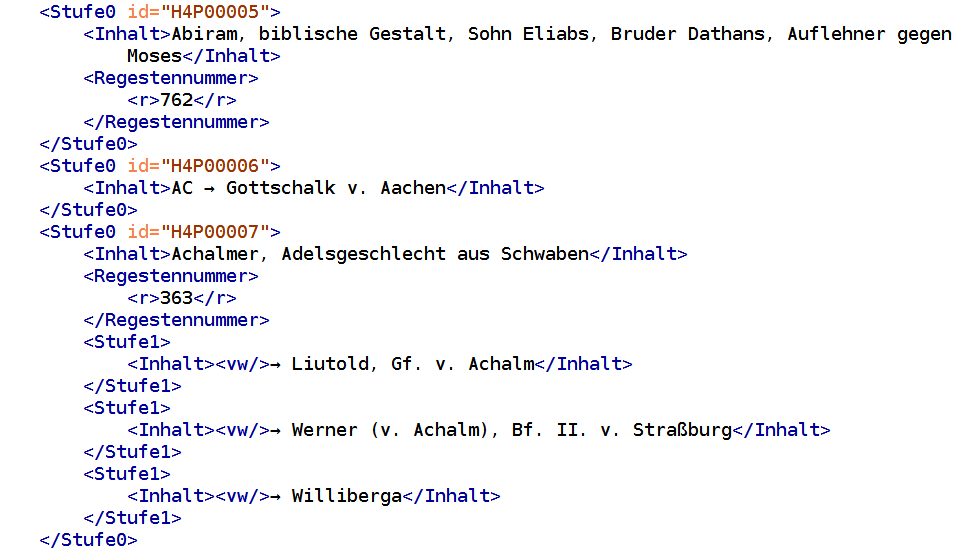
\includegraphics{Bilder/RI2Graph/XML-Register.png}
\caption{Ausschnitt aus dem XML-Register der Regesten Heinrichs IV.}
\end{figure}

In der XML-Fassung sind die inhaltlichen Bereiche und die Abschnitte für die Regestennummern jeweils extra in die Tags \texttt{\textless{}Inhalt} und \texttt{Regestennummer} eingefasst. Innerhalb des Elements \texttt{Regestennummer} ist dann nochmal jede einzelne Regestennummer in \texttt{\textless{}r\textgreater{}}-Tags eingefasst. Die aus dem gedruckten Register übernommenen Verweise sind durch ein leeres \texttt{\textless{}vw/\textgreater{}}-Element gekennzeichnet.

Die in XML vorliegenden Registerdaten werden anschließend mit Hilfe von TuStep in einzelne CSV-Tabellen zerlegt.

\begin{figure}
\centering
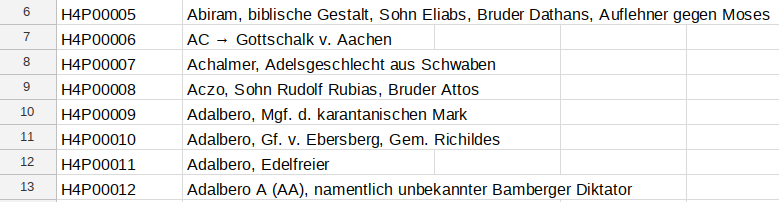
\includegraphics{Bilder/RI2Graph/RegisterH4-Tabelle-Entitaeten.png}
\caption{Ausschnitt der Entitätentabelle des Registers der Regesten Heinrichs IV.}
\end{figure}

In einer Tabelle werden alle Entitäten aufgelistet und jeweils mit einer ID versehen.

\begin{figure}
\centering
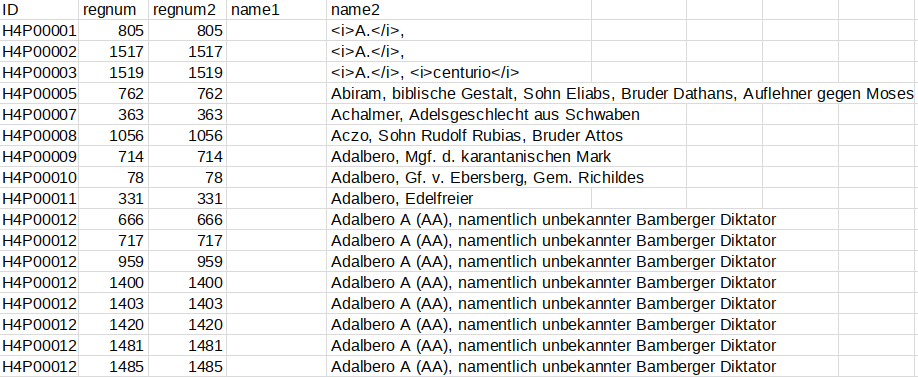
\includegraphics{Bilder/RI2Graph/RegisterH4-GENANNT.png}
\caption{Ausschnitt der Verknüpfungstabelle des Registers der Regesten Heinrichs IV.}
\end{figure}

In der anderen Tabelle werden die Verknüpfungen zwischen Registereinträgen und den Regesten aufgelistet. Der Registereintrag Adalbero kommt also in mehreren Regesten vor. Da das Register der Regesten Heinrichs IV. nur zwei Hierarchiestufen enthält, in denen beispielsweise verschiedene Amtsphasen ein und derselben Person unterschieden werden, wurden diese beim Import zusammengefasst.\footnote{Vgl. die Vorbemerkung zum Register in Böhmer, J. F., Regesta Imperii III. Salisches Haus 1024-1125. Tl. 2: 1056-1125. 3. Abt.: Die Regesten des Kaiserreichs unter Heinrich IV. 1056 (1050) - 1106. 5. Lief.: Die Regesten Rudolfs von Rheinfelden, Hermanns von Salm und Konrads (III.). Verzeichnisse, Register, Addenda und Corrigenda, bearbeitet von Lubich, Gerhard unter Mitwirkung von Junker, Cathrin; Klocke, Lisa und Keller, Markus - Köln (u.a.) (2018), S. 291.} Damit gibt es pro Person jeweils nur einen Knoten.

\subsection{Import der Registerdaten in die Graphdatenbank}\label{import-der-registerdaten-in-die-graphdatenbank-1}

Im Gegensatz zu den Regesten Kaiser Friedrichs III., bei denen Orte und Personen in einem Register zusammengefasst sind, haben die Regesten Kaiser Heinrich IV. getrennte Orts- und Personenregister. Die digitalisierten Registerdaten können \href{https://docs.google.com/spreadsheets/d/12T-RD1Ct4aAUNNNxipjMmHe9F1NmryI1gf8_SJ4RCEE/edit?usp=sharing}{hier} eingesehen werden. In dem Tabellendokument befinden sich insgesamt drei Tabellen. In der Tabelle Personen sind die Einträge des Personenregisters aufgelistet und in der Tabelle Orte befindet sich die Liste aller Einträge des Ortsregisters. Schließlich enthält die Tabelle \texttt{APPEARS\_IN} Information dazu, welche Personen oder Orte in welchen Regesten genannt sind. Der folgende cypher-Query importiert die Einträge der Personentabelle in die Graphdatenbank und erstellt für jeden Eintrag einen Knoten vom Typ \texttt{:IndexPerson}:

\begin{verbatim}
// Registereinträge Personen erstellen
LOAD CSV WITH HEADERS FROM "https://docs.google.com/spreadsheets/d/12T-RD1Ct4aAUNNNxipjMmHe9F1NmryI1gf8_SJ4RCEE/export?format=csv&id=12T-RD1Ct4aAUNNNxipjMmHe9F1NmryI1gf8_SJ4RCEE&gid=1167029283"
AS line
CREATE (:IndexPerson {registerId:line.ID, name1:line.name1});
\end{verbatim}

Mit dem folgenden cypher-Query werden nach dem gleichen Muster aus der Tabelle \texttt{Orte} die Ortseinträge in die Graphdatenbank importiert.

\begin{verbatim}
// Registereinträge Orte erstellen
LOAD CSV WITH HEADERS FROM "https://docs.google.com/spreadsheets/d/12T-RD1Ct4aAUNNNxipjMmHe9F1NmryI1gf8_SJ4RCEE/export?format=csv&id=12T-RD1Ct4aAUNNNxipjMmHe9F1NmryI1gf8_SJ4RCEE&gid=2049106817"
AS line
CREATE (:IndexPlace {registerId:line.ID, name1:line.name1});
\end{verbatim}

Die beiden Befehle greifen also auf verschiedene Tabellenblätter des gleichen Google-Tabellendokuments zu, laden es als CSV-Daten und übergeben die Daten zeilenweise an die weiteren Befehle (Hier an den \texttt{MATCH}- und den \texttt{CREATE}-Befehl). Im nächsten Schritt werden nun mit den Daten der \texttt{APPEARS\_IN}-Tabelle die Verknüpfungen zwischen den Registereinträgen und den Regesten erstellt.

\begin{verbatim}
// PLACE_IN-Kanten für Orte erstellen
LOAD CSV WITH HEADERS FROM "https://docs.google.com/spreadsheets/d/12T-RD1Ct4aAUNNNxipjMmHe9F1NmryI1gf8_SJ4RCEE/export?format=csv&id=12T-RD1Ct4aAUNNNxipjMmHe9F1NmryI1gf8_SJ4RCEE&gid=2147130316"
AS line
MATCH (from:IndexPlace {registerId:line.ID})
MATCH (to:Regesta {regnum:line.regnum2})
CREATE (from)-[:PLACE_IN {regnum:line.regnum, name1:line.name1, name2:line.name2}]->(to);
\end{verbatim}

Mit zwei \texttt{MATCH}-Befehlen wird jeweils das Regest und der Registereintrag aufgerufen und mit dem \texttt{CREATE}-Befehl eine \texttt{PLACE\_IN}-Kante zwischen den beiden Knoten angelegt, die als Attribute den Inhalt der Spalten \texttt{name1} und \texttt{name2} erhält. Analog werden die Verknüpfungen zwischen Regestenknoten und Personenknoten angelegt:

\begin{verbatim}
// PERSON_IN-Kanten für Person erstellen
LOAD CSV WITH HEADERS FROM "https://docs.google.com/spreadsheets/d/12T-RD1Ct4aAUNNNxipjMmHe9F1NmryI1gf8_SJ4RCEE/export?format=csv&id=12T-RD1Ct4aAUNNNxipjMmHe9F1NmryI1gf8_SJ4RCEE&gid=2147130316"
AS line
MATCH (from:IndexPerson {registerId:line.ID}), (to:Regesta {regnum:line.regnum2})
CREATE (from)-[:PERSON_IN {regnum:line.regnum, name1:line.name1, name2:line.name2}]->(to);
\end{verbatim}

\subsection{Die Hierarchie des Registers der Regesten Kaiser Friedrichs III.}\label{die-hierarchie-des-registers-der-regesten-kaiser-friedrichs-iii.}

In anderen Registern der Regesta Imperii, wie beispielsweise den Regesten Kaiser Friedrichs III., sind teilweise fünf oder mehr Hierarchiestufen vorhanden, die jeweils auch Entitäten repräsentieren. In diesen Fällen müssen die Hierarchien auch in der Graphdatenbank abgebildet werden, was durch zusätzliche Verweise auf die ggf. vorhandenen übergeordneten Registereinträge möglich wird.

\begin{figure}
\centering
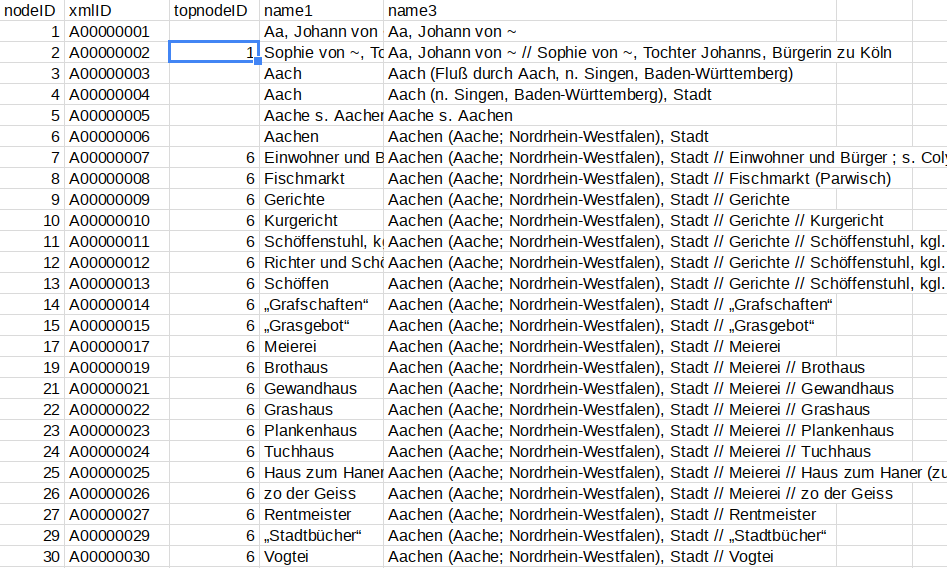
\includegraphics{Bilder/RI2Graph/RegisterF3-Hierarchie.png}
\caption{Ausschnitt der Entitätentabelle des Registers der Regesten Friedrichs III.}
\end{figure}

Im Tabellenausschnitt wird jedem Registereintrag in der ersten Spalte eine \texttt{nodeID} als eindeutige Kennung zugewiesen. Bei Registereinträgen, die kein Hauptlemma sind, enthält die dritte Spalte \texttt{topnodeID} den Verweis auf die eindeutige Kennung \texttt{nodeID} des übergeordneten Eintrages. Beim Import in die Graphdatenbank wird diese Hierarchie über \texttt{CHILD\_OF}-Kanten abgebildet, die vom untergeordneten Eintrag auf das übergeordnete Lemma verweisen. Damit ist die komplette Registerhierarchie im Graphen abgebildet. In der Spalte \texttt{name1} ist das Lemma angegeben. In der Spalte \texttt{name3} ist zusätzlich zum Lemma noch der gesamte Pfad vom Hauptlemma bis zum Registereintrag, jeweils mit Doppelslahes (\texttt{//}) getrennt. Bei tiefer gestaffelten Registern ist teilweise ohne Kenntnis der übergeordneten Einträge eine eindeutige Identifizierung eines Eintrages nicht möglich. So wird in Zeile 17 der o.a. Abbildung allein mit der Angabe aus der Spalte \texttt{name1} nicht klar, um welche \texttt{Meierei} es sich handelt. Mit dem kompletten Pfad des Registereintrages in der Spalte \texttt{name3} wird dagegen deutlich, dass die Aachener \texttt{Meierei} gemeint ist.

\section{Auswertungsperspektiven}\label{auswertungsperspektiven}

\subsection{Personennetzwerke in den Registern}\label{personennetzwerke-in-den-registern}

\subsubsection{Graf Robert II. von Flandern in seinem Netzwerk}\label{graf-robert-ii.-von-flandern-in-seinem-netzwerk}

Nach dem Import können nun die Online-Regesten und die Informationen aus den Registern der Regesten Kaiser Heinrichs IV. in einer Graphdatenbank aus einer Vernetzungsperspektive abgefragt werden.\footnote{Die nun folgenden Abfragen sind zum Teil einer Präsentation entnommen, die für die Summerschool der \href{https://www.digitale-akademie.de}{Digitalen Akademie} im Rahmen des \href{https://www.mainzed.org/de}{Mainzed} entwickelt wurden. Die Präsentation findet sich unter der URL \url{https://digitale-methodik.adwmainz.net/mod5/5c/slides/graphentechnologien/RI.html}.}

Ausgangspunkt ist der Registereintrag von \href{https://de.wikipedia.org/wiki/Robert_II._(Flandern)}{Graf Robert II. von Flandern}. Diesen Knoten finden wir mit folgendem Query.

\begin{verbatim}
// Robert II. von Flandern
MATCH (n:IndexPerson) WHERE n.registerId = 'H4P01822'
RETURN *;
\end{verbatim}

Mit einem Doppelklick auf den \texttt{IndexPerson}-Knoten öffnen sich alle \texttt{Regesta}-Knoten, in denen Robert genannt ist. Klickt man nun wiederum alle Regestenknoten doppelt an, sieht man alle Personen und Orte, mit denen Robert gemeinsam in den Regesten genannt ist.

Dies kann auch in einem cypher-Query zusammengefasst werden.

\begin{verbatim}
// Robert II. von Flandern mit Netzwerk
MATCH (n:IndexPerson)-[:PERSON_IN]->
(r:Regesta)<-[:PERSON_IN]-
(m:IndexPerson)
WHERE n.registerId = 'H4P01822'
RETURN *;
\end{verbatim}

In der folgenden Abb. wird das Ergebnis dargestellt.

\begin{figure}
\centering
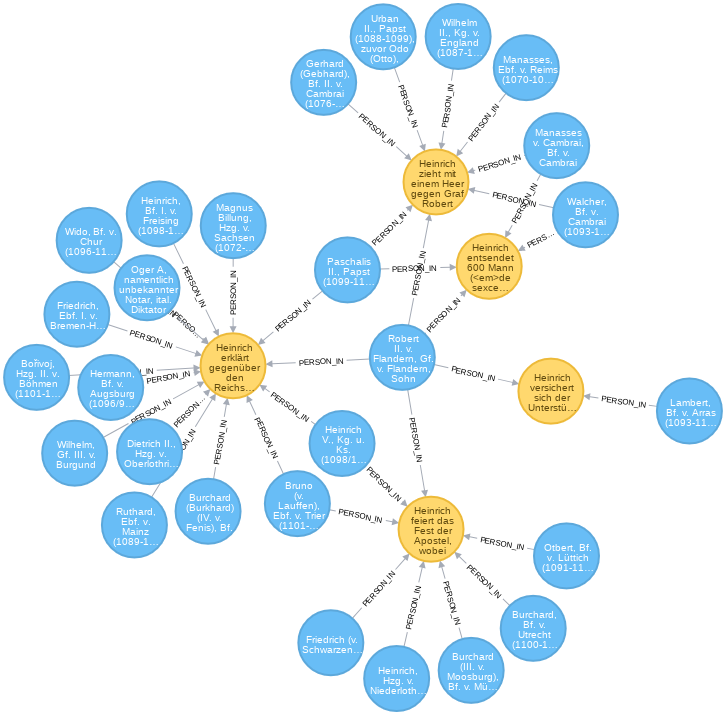
\includegraphics{Bilder/RI2Graph/RobertVonFlandernMitRegesten.png}
\caption{Robert mit den Personen, mit denen er gemeinsam in Regesten genannt wird.}
\end{figure}

Hier wird der \texttt{MATCH}-Befehl um einen Pfad über \texttt{PERSON\_IN}-Kanten zu \texttt{Regesta}-Knoten ergänzt, von denen jeweils eine \texttt{PERSON\_IN}-Kante zu den anderen, in den Regesten genannten \texttt{IndexPerson}-Knoten führt.

Nimmt man noch eine weitere Ebene hinzu, wächst die Ergebnismenge stark an. Der folgende Query kann daher je nach Rechnerleistung etwas länger dauern.

\begin{verbatim}
// Robert II. von Flandern mit Netzwerk und Herrscherhandeln (viel)
MATCH
(n1:IndexPerson)-[:PERSON_IN]->(r1:Regesta)<-[:PERSON_IN]-
(n2:IndexPerson)-[:PERSON_IN]->(r2:Regesta)<-[:PERSON_IN]-
(n3:IndexPerson)
WHERE n1.registerId = 'H4P01822'
RETURN *;
\end{verbatim}

\begin{figure}
\centering
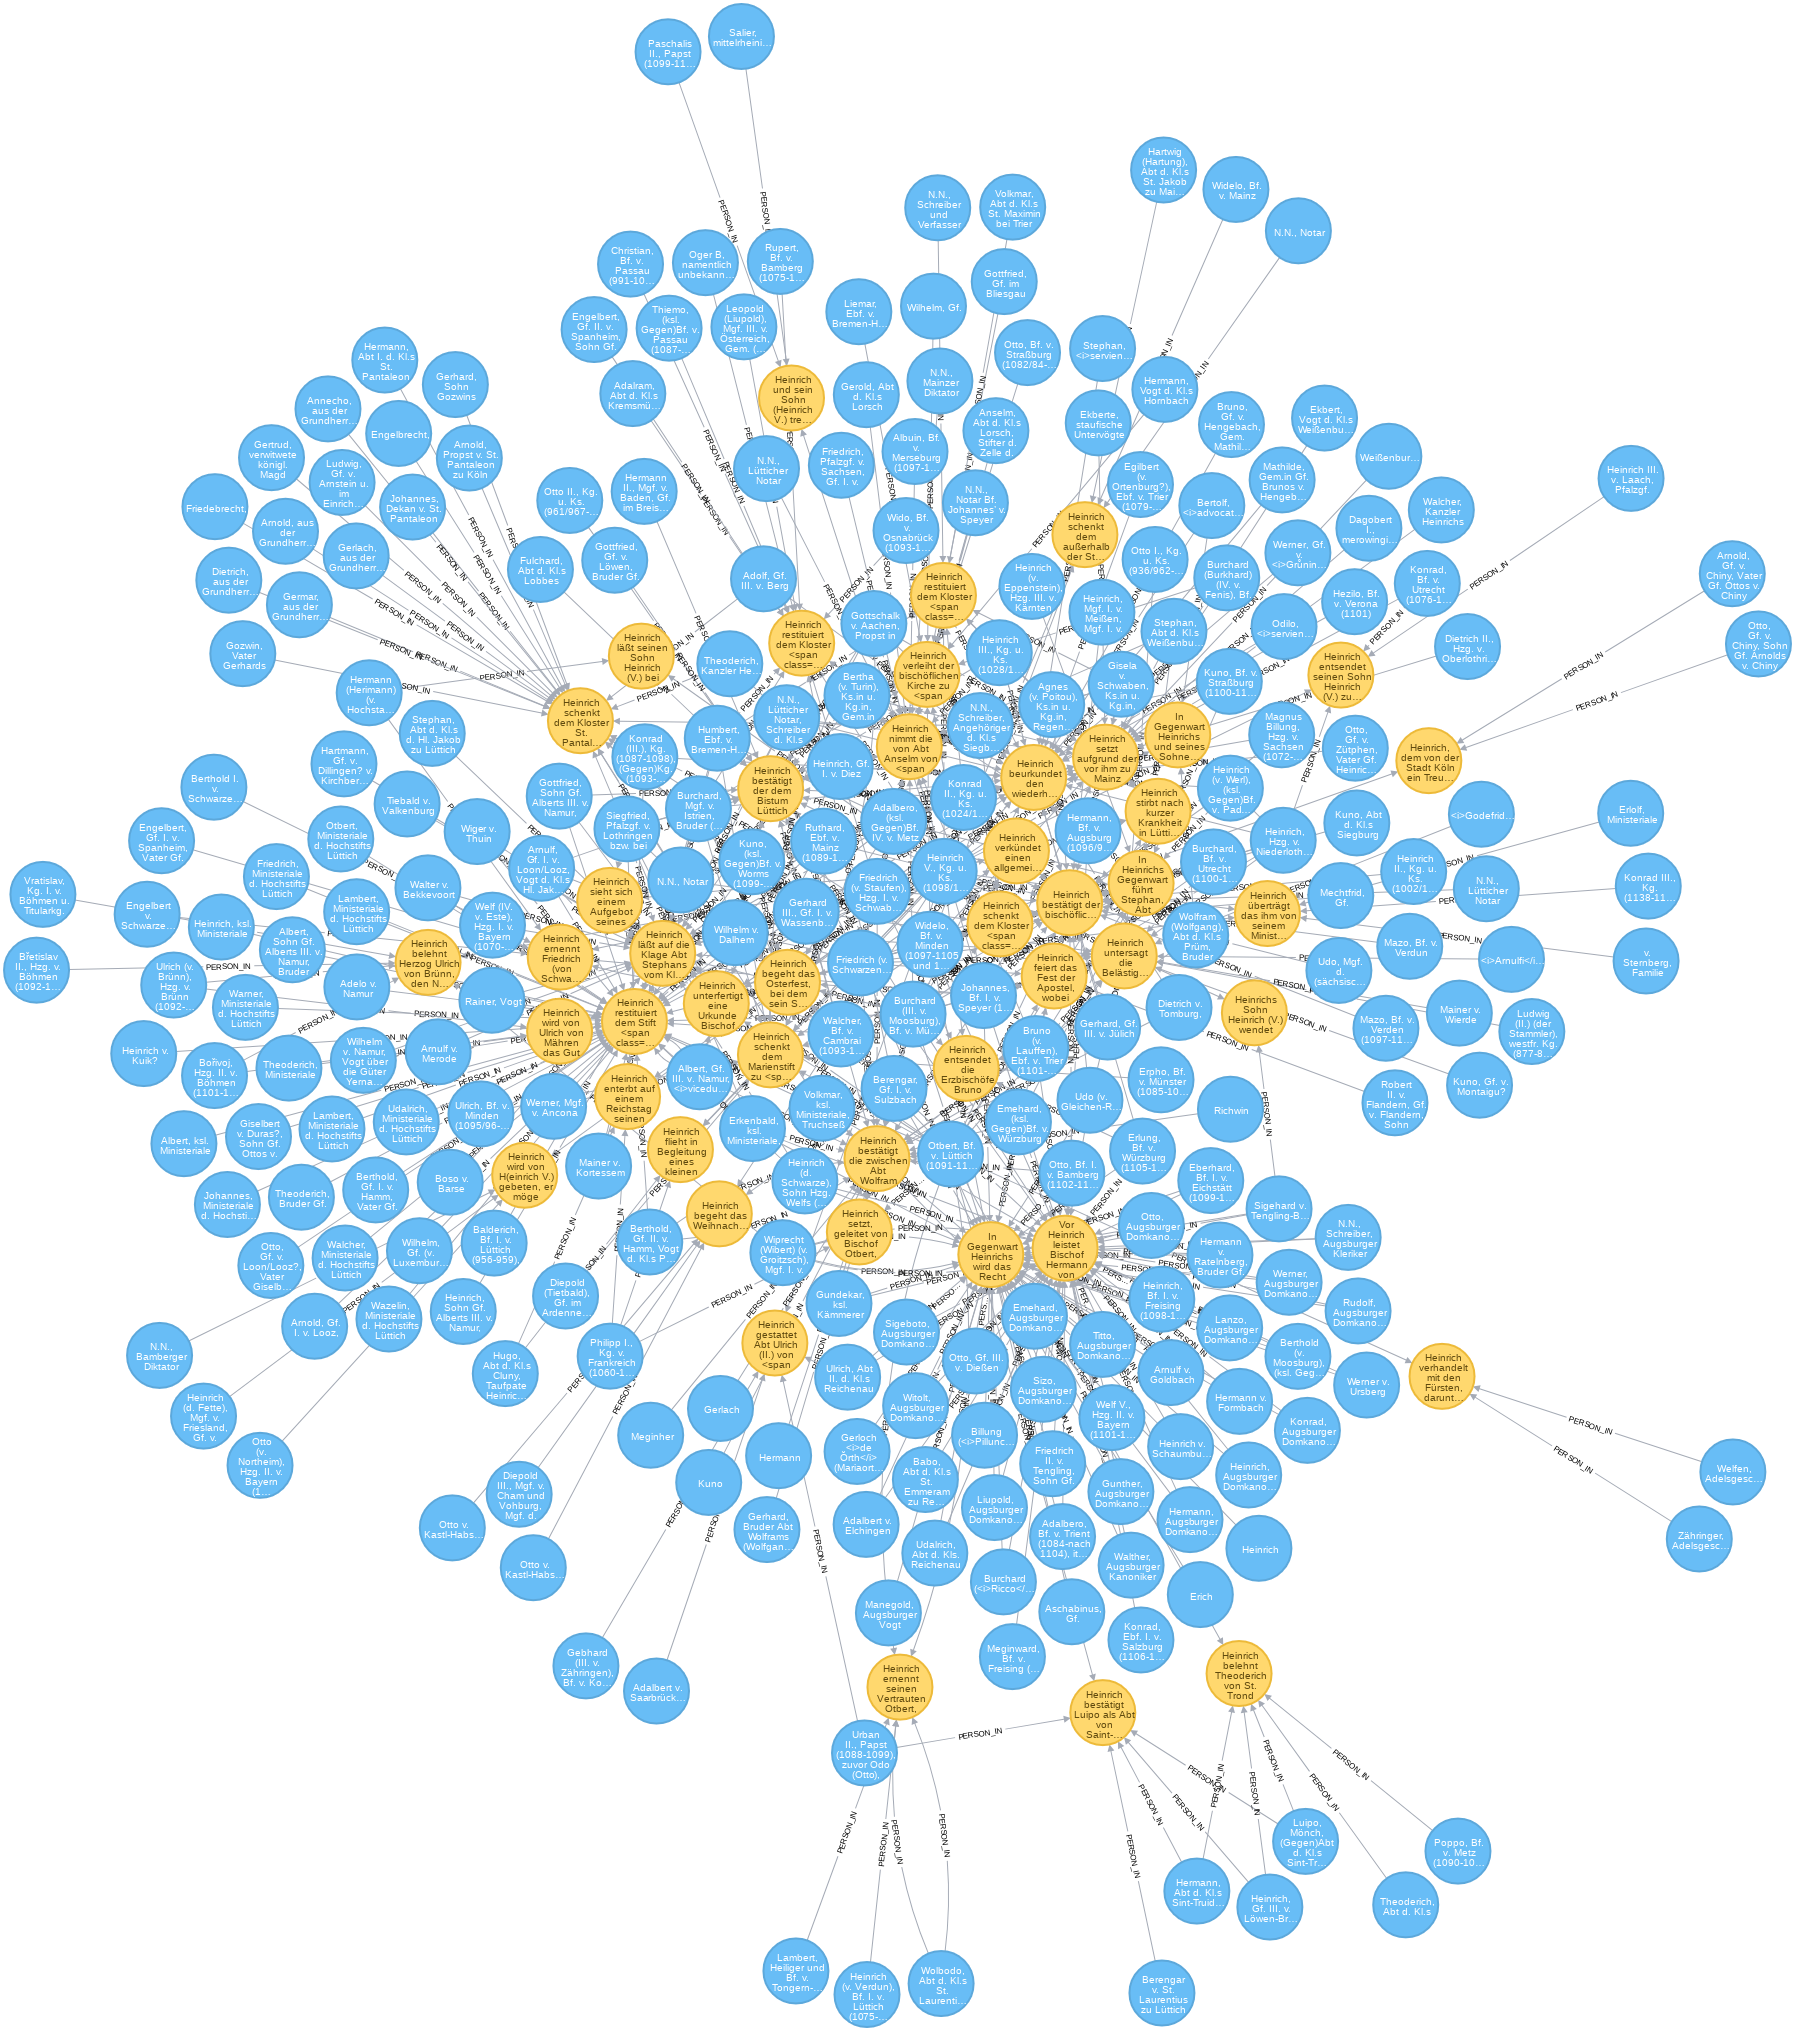
\includegraphics{Bilder/RI2Graph/Robert-viel.png}
\caption{Robert mit Personen, die wiederum mit Personen gemeinsam in Regesten genannt sind.}
\end{figure}

\subsubsection{Graf Robert II. von Flandern und Herzog Heinrich von Niederlothringen}\label{graf-robert-ii.-von-flandern-und-herzog-heinrich-von-niederlothringen}

In der Graphdatenbank ist es über die Exploration der Beziehungen einer Person hinaus möglich, explizit die Verbindungen von zwei Personen abzufragen. In unserem nächsten Beispiel suchen wir jene Regesten, in denen \href{https://de.wikipedia.org/wiki/Robert_II._(Flandern)}{Graf Robert II. von Flandern} und \href{https://de.wikipedia.org/wiki/Heinrich_I._(Limburg)}{Herzog Heinrich von Niederlothringen} gemeinsam genannt sind.

\begin{verbatim}
// Robert II. von Flandern und Herzog Heinrich von Niederlothringen mit Netzwerk
MATCH
(n:IndexPerson)-[:PERSON_IN]->
(r:Regesta)<-[:PERSON_IN]-(m:IndexPerson)
WHERE n.registerId = 'H4P01822'
AND m.registerId = 'H4P00926'
RETURN *;
\end{verbatim}

\begin{figure}
\centering
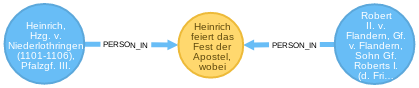
\includegraphics{Bilder/RI2Graph/RobertundHeinrich.png}
\caption{Robert und Heinrich sind in einem Regest gemeinsam genannt.}
\end{figure}

Es zeigt sich, dass Robert und Heinrich in einem Regest gemeinsam genannt sind.

Und dieses \href{http://www.regesta-imperii.de/id/cf75356b-bd0d-4a67-8aeb-3ae27d1dcefa}{Regest} berichtet von der Unterwerfung Roberts unter und Heinrich IV.\footnote{Vgl. RI III,2,3 n. 1487.}

\begin{quote}
Heinrich feiert das Fest der Apostel, wobei sich Graf Robert von Flandern im Beisein mehrerer Fürsten unterwirft, namentlich der Erzbischöfe Friedrich von Köln und Bruno von Trier, der Bischöfe Otbert von Lüttich, Burchard von Münster, Burchard von Utrecht, Herzog Heinrich von Niederlothringen sowie mehrerer Grafen.
\end{quote}

Möglicherweise haben beide aber gemeinsame Bekannte, also Personen mit denen sowohl Heinrich als auch Robert in unterschiedlichen Regesten gemeinsam genannt sind. Hierfür wird der cypher-Query um eine Ebende erweitert.

\begin{verbatim}
// Robert und Heinrich mit allen gemeinsamen Personen und Regesten
MATCH (n1:IndexPerson)
-[:PERSON_IN]->(r1:Regesta)<-[:PERSON_IN]-
(n2:IndexPerson)-[:PERSON_IN]->(r2:Regesta)
<-[:PERSON_IN]-(n3:IndexPerson)
WHERE n1.registerId = 'H4P00926'
AND n3.registerId = 'H4P01822'
RETURN *;
\end{verbatim}

\begin{figure}
\centering
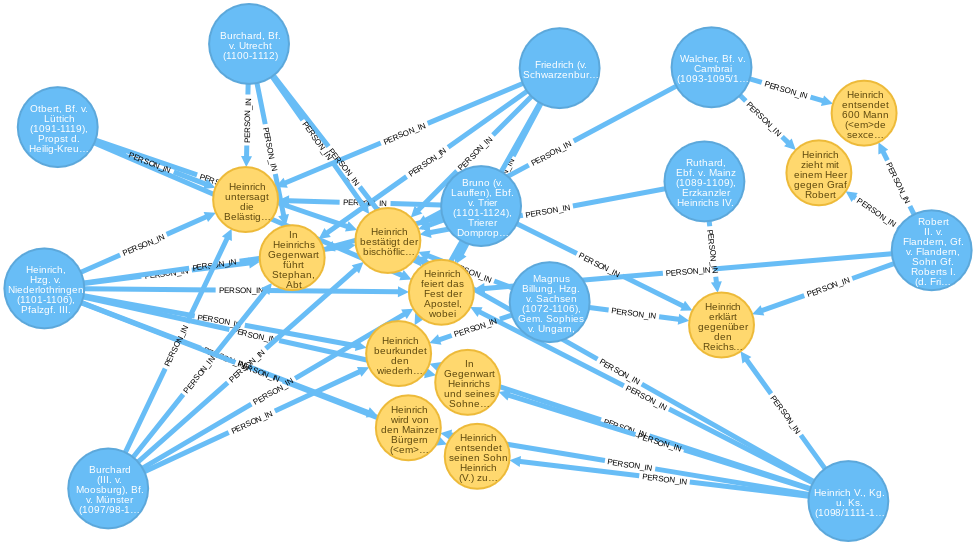
\includegraphics{Bilder/RI2Graph/RobertundHeinrichMitBrokern.png}
\caption{Robert und Heinrich mit den gemeinsamen Bekanntschaften.}
\end{figure}

Ein erster Blick auf das Ergebnis zeigt, dass Heinrich allgemein besser vernetzt ist. Für die weitere Analyse ihres Verhältnisses ist nun die Lektüre der angegebenen Regesten notwendig. Hierfür lässt sich das Ergebnis noch etwas weiter aufbereiten, indem die zwischen den Personen liegenden Regesten in \texttt{KNOWS}-Kanten umgewandelt werden, die als zusätzliche Information die Angaben zu den Regesten enthalten.

\begin{verbatim}
// Rausrechnen der dazwischenliegenden Knoten
MATCH
(startPerson:IndexPerson)-[:PERSON_IN]->
(regest:Regesta)<-[:PERSON_IN]-(endPerson:IndexPerson)
WHERE startPerson.registerId in ['H4P01822', 'H4P00926']
WITH startPerson, endPerson, count(regest) as anzahl,
collect(regest.ident) as idents
CALL apoc.create.vRelationship(startPerson, "KNOWS",
{anzahl:anzahl, regesten:idents}, endPerson) YIELD rel
RETURN startPerson, endPerson, rel;
\end{verbatim}

\begin{figure}
\centering
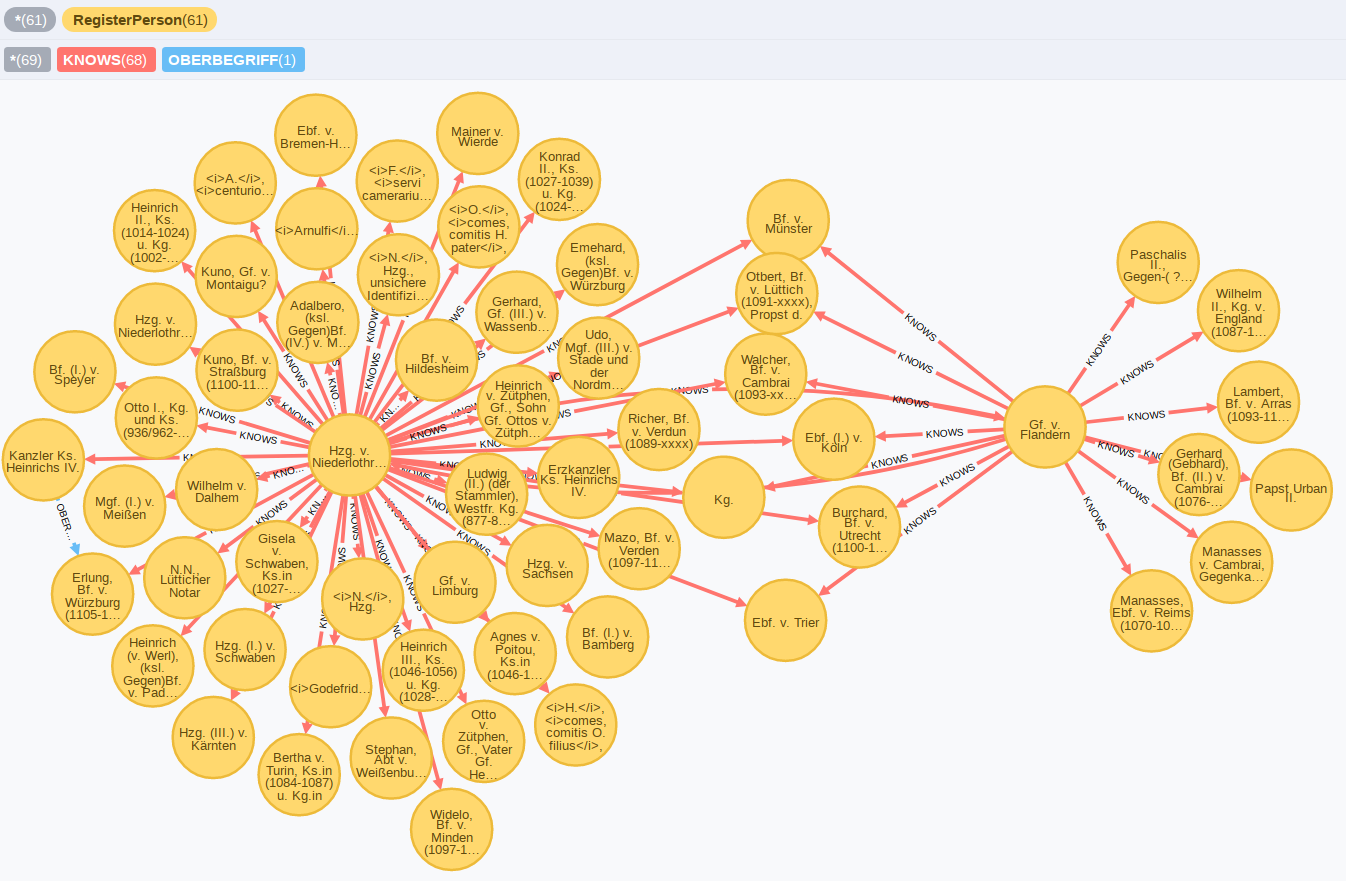
\includegraphics{Bilder/RI2Graph/RobertUndHeinrichApoc.png}
\caption{Robert und Heinrich mit den gemeinsamen Bekanntschaften.}
\end{figure}

In der Abbildung sind die zwei Ego-Netzwerke von Heinrich (links) und Robert (rechts) mit den dazwischen liegenden gemeinsamen Bekanntschaften dargestellt. Es zeigt sich, dass Heinrich stärker sowohl mit Geistlichen als auch Weltlichen vernetzt war, während Robert insgesamt weniger Kontakte aber mit einem Schwerpunkt in der Geistlichkeit hatte.

Für den Historiker ist aber vor allem interessant, was in den Regesten steht, die Robert und Heinrich über die Mittelsmänner verbinden. Hierfür wird der cypher-Query angepasst und sowohl Personen als auch die Regestentexte ausgegeben.

\begin{verbatim}
// Liste der Regesten als Ergebnis
MATCH
(startPerson:IndexPerson)-[:PERSON_IN]->
(regest1:Regesta)<-[:PERSON_IN]-(middlePerson:IndexPerson)
-[:PERSON_IN]->(regest2:Regesta)
<-[:PERSON_IN]-(endPerson:IndexPerson)
WHERE startPerson.registerId in ['H4P00926']
AND endPerson.registerId in ['H4P01822']
RETURN DISTINCT startPerson.name1,
regest1.ident, regest1.text,
middlePerson.name1, regest2.ident,
regest2.text, endPerson.name1;
\end{verbatim}

In der folgenden Abbildung wird ein Ausschnitt der Ergebnistabelle gezeigt. In der ersten Spalte der Tabelle finden sich Robert, anschließend die Angaben zum Regest, mit dem er mit der mitteleren Person (middlePerson.name1) verknüpft ist. Dem folgen schließlich die Angaben zum Regest, mit den die mittlere Person mit Robert in der letzten Spalte verbunden ist. Die Tabelle bietet einen Überblick zur Überlieferungssituation aus der Perspektive der Regesta Imperii.

\begin{figure}
\centering
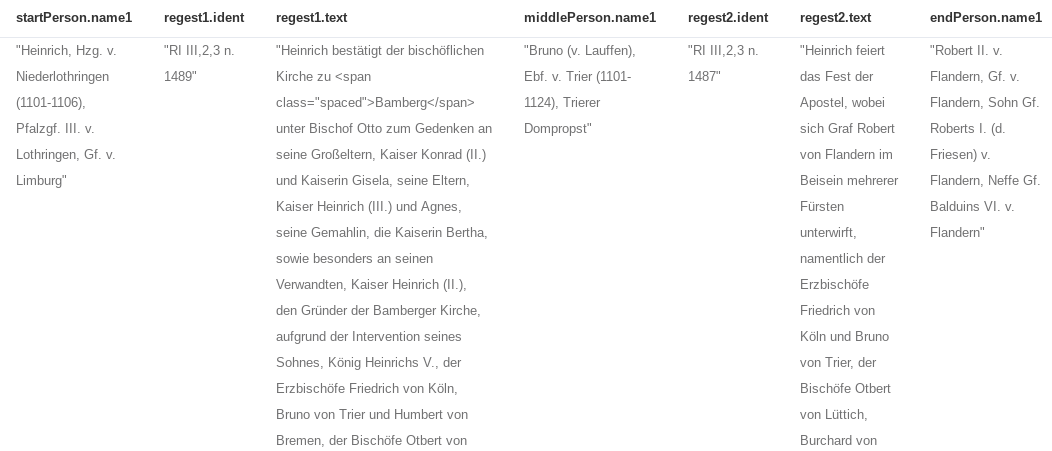
\includegraphics{Bilder/RI2Graph/RobertHeinrichApocTabelle.png}
\caption{Robert und Heinrich mit den gemeinsamen Bekanntschaften.}
\end{figure}

\subsection{Herrscherhandeln ausgezählt}\label{herrscherhandeln-ausgezuxe4hlt}

Wie bereits oben erwähnt wurde in einem ersten Test jeweils das erste Verb des Regestentextes extrahiert, lemmatisiert und in die Graphdatenbank eingespielt. Im folgenden werden nun einige cypher-Querys vorgestellt, die dies beispielhaft auswerten.

\begin{verbatim}
// Herrscherhandeln ausgezählt
MATCH (n:Lemma)<-[h:ACTION]-(m:Regesta)
RETURN n.lemma, count(h) as ANZAHL ORDER BY ANZAHL desc LIMIT 10;
\end{verbatim}

\begin{longtable}[]{@{}ll@{}}
\toprule
n.lemma & ANZAHL\tabularnewline
\midrule
\endhead
werden & 145\tabularnewline
schenken & 133\tabularnewline
bestätigen & 109\tabularnewline
begehen & 95\tabularnewline
verleihen & 48\tabularnewline
ernennen & 36\tabularnewline
nehmen & 35\tabularnewline
treffen & 34\tabularnewline
empfangen & 29\tabularnewline
erhalten & 26\tabularnewline
\bottomrule
\end{longtable}

Die Ergebnisliste zeigt gleich die Einschränkungen, da das Hilfsverb \emph{werden} aus dem textuellen Zusammenhang gerissen ist. Andererseits ergeben sich aber auch interessante Erkenntnisse zur Häufigkeitsverteilung von Herrscherhandeln in Regestentexten. Die Anwendung des Verfahrens auf Regestentexte ist dabei auf der einen Seite positiv, da bei der Erstellung der Regesten sehr stark auf formale Kriterien geachtet wird und so die Zusammenhänge gut zu erfassen sind. Auf der anderen Seite ist die Auswertung aber wiederum einen weiteren Schritt von der ursprünglichen Quelle entfernt.

\subsection{Herrscherhandeln pro Ausstellungsort ausgezählt}\label{herrscherhandeln-pro-ausstellungsort-ausgezuxe4hlt}

Im folgenden Query kommt eine räumliche Komponente zur Abfrage hinzu, da das Lemma hier jeweils abhängig vom Ausstellungsort der Urkunde abgefragt wird.

\begin{verbatim}
// Herrscherhandeln pro Ausstellungsort
MATCH (n:Lemma)<-[h:ACTION]-(:Regesta)-[:PLACE_OF_ISSUE]->(p:Place)
WHERE p.normalizedGerman IS NOT NULL
RETURN p.normalizedGerman, n.lemma, count(h) as ANZAHL ORDER BY ANZAHL desc LIMIT 10;
\end{verbatim}

\begin{longtable}[]{@{}lrr@{}}
\toprule
p.normalizedGerman & n.lemma & ANZAHL\tabularnewline
\midrule
\endhead
Mainz & begehen & 15\tabularnewline
Mainz & schenken & 14\tabularnewline
Goslar & schenken & 13\tabularnewline
Rom & werden & 12\tabularnewline
Regensburg & schenken & 12\tabularnewline
Goslar & begehen & 11\tabularnewline
Speyer & schenken & 10\tabularnewline
Worms & begehen & 8\tabularnewline
Regensburg & bestätigen & 7\tabularnewline
Regensburg & werden & 7\tabularnewline
\bottomrule
\end{longtable}

In der ersten Spalte befindet sich der Ortsname, der aus der Property \texttt{normalizedGerman} des \texttt{Place}-Knotens stammt. In der zweiten Spalte wird das Lemma angegeben und in der dritten Spalte schließlich die Anzahl der jeweiligen Regesten. Interessant wäre hier auch noch die Ergänzung der zeitlichen Dimension, mit der dann der zeitliche Verlauf in die Auswertung miteinbezogen werden könnte.

\subsection{Herrscherhandeln und Anwesenheit}\label{herrscherhandeln-und-anwesenheit}

Im nächsten Beispiel werden in einem Regest genannten Personen in die Auswertung des Herrscherhandelns mit einbezogen.

\begin{verbatim}
MATCH (p:IndexPerson)-[:PERSON_IN]-(r:Regesta)-[:ACTION]-(l:Lemma)
RETURN p.name1, l.lemma, count(l) AS Anzahl ORDER BY p.name1, Anzahl DESC;
\end{verbatim}

\begin{longtable}[]{@{}lrr@{}}
\toprule
\begin{minipage}[b]{0.06\columnwidth}\raggedright\strut
p.name1\strut
\end{minipage} & \begin{minipage}[b]{0.06\columnwidth}\raggedleft\strut
l.lemma\strut
\end{minipage} & \begin{minipage}[b]{0.06\columnwidth}\raggedleft\strut
Anzahl\strut
\end{minipage}\tabularnewline
\midrule
\endhead
\begin{minipage}[t]{0.06\columnwidth}\raggedright\strut
\ldots{}\strut
\end{minipage} & \begin{minipage}[t]{0.06\columnwidth}\raggedleft\strut
\ldots{}\strut
\end{minipage} & \begin{minipage}[t]{0.06\columnwidth}\raggedleft\strut
\ldots{}\strut
\end{minipage}\tabularnewline
\begin{minipage}[t]{0.06\columnwidth}\raggedright\strut
Adalbero, Metzer Domkanoniker, Kanzler Heinrichs IV., Kanzler (Gegen)Kg. Rudolfs v. Rheinfelden\strut
\end{minipage} & \begin{minipage}[t]{0.06\columnwidth}\raggedleft\strut
schenken\strut
\end{minipage} & \begin{minipage}[t]{0.06\columnwidth}\raggedleft\strut
21\strut
\end{minipage}\tabularnewline
\begin{minipage}[t]{0.06\columnwidth}\raggedright\strut
Adalbero, Metzer Domkanoniker, Kanzler Heinrichs IV., Kanzler (Gegen)Kg. Rudolfs v. Rheinfelden\strut
\end{minipage} & \begin{minipage}[t]{0.06\columnwidth}\raggedleft\strut
bestätigen\strut
\end{minipage} & \begin{minipage}[t]{0.06\columnwidth}\raggedleft\strut
9\strut
\end{minipage}\tabularnewline
\begin{minipage}[t]{0.06\columnwidth}\raggedright\strut
Adalbero, Metzer Domkanoniker, Kanzler Heinrichs IV., Kanzler (Gegen)Kg. Rudolfs v. Rheinfelden\strut
\end{minipage} & \begin{minipage}[t]{0.06\columnwidth}\raggedleft\strut
verleihen\strut
\end{minipage} & \begin{minipage}[t]{0.06\columnwidth}\raggedleft\strut
4\strut
\end{minipage}\tabularnewline
\begin{minipage}[t]{0.06\columnwidth}\raggedright\strut
Adalbero, Metzer Domkanoniker, Kanzler Heinrichs IV., Kanzler (Gegen)Kg. Rudolfs v. Rheinfelden\strut
\end{minipage} & \begin{minipage}[t]{0.06\columnwidth}\raggedleft\strut
erlassen\strut
\end{minipage} & \begin{minipage}[t]{0.06\columnwidth}\raggedleft\strut
2\strut
\end{minipage}\tabularnewline
\begin{minipage}[t]{0.06\columnwidth}\raggedright\strut
Adalbero, Metzer Domkanoniker, Kanzler Heinrichs IV., Kanzler (Gegen)Kg. Rudolfs v. Rheinfelden\strut
\end{minipage} & \begin{minipage}[t]{0.06\columnwidth}\raggedleft\strut
übertragen\strut
\end{minipage} & \begin{minipage}[t]{0.06\columnwidth}\raggedleft\strut
2\strut
\end{minipage}\tabularnewline
\begin{minipage}[t]{0.06\columnwidth}\raggedright\strut
Adalbero, Metzer Domkanoniker, Kanzler Heinrichs IV., Kanzler (Gegen)Kg. Rudolfs v. Rheinfelden\strut
\end{minipage} & \begin{minipage}[t]{0.06\columnwidth}\raggedleft\strut
ermäßigen\strut
\end{minipage} & \begin{minipage}[t]{0.06\columnwidth}\raggedleft\strut
2\strut
\end{minipage}\tabularnewline
\begin{minipage}[t]{0.06\columnwidth}\raggedright\strut
Adalbero, Metzer Domkanoniker, Kanzler Heinrichs IV., Kanzler (Gegen)Kg. Rudolfs v. Rheinfelden\strut
\end{minipage} & \begin{minipage}[t]{0.06\columnwidth}\raggedleft\strut
gestatten\strut
\end{minipage} & \begin{minipage}[t]{0.06\columnwidth}\raggedleft\strut
2\strut
\end{minipage}\tabularnewline
\begin{minipage}[t]{0.06\columnwidth}\raggedright\strut
Adalbero, Metzer Domkanoniker, Kanzler Heinrichs IV., Kanzler (Gegen)Kg. Rudolfs v. Rheinfelden\strut
\end{minipage} & \begin{minipage}[t]{0.06\columnwidth}\raggedleft\strut
vollziehen\strut
\end{minipage} & \begin{minipage}[t]{0.06\columnwidth}\raggedleft\strut
1\strut
\end{minipage}\tabularnewline
\begin{minipage}[t]{0.06\columnwidth}\raggedright\strut
Adalbero, Metzer Domkanoniker, Kanzler Heinrichs IV., Kanzler (Gegen)Kg. Rudolfs v. Rheinfelden\strut
\end{minipage} & \begin{minipage}[t]{0.06\columnwidth}\raggedleft\strut
nehmen\strut
\end{minipage} & \begin{minipage}[t]{0.06\columnwidth}\raggedleft\strut
1\strut
\end{minipage}\tabularnewline
\begin{minipage}[t]{0.06\columnwidth}\raggedright\strut
Adalbero, Metzer Domkanoniker, Kanzler Heinrichs IV., Kanzler (Gegen)Kg. Rudolfs v. Rheinfelden\strut
\end{minipage} & \begin{minipage}[t]{0.06\columnwidth}\raggedleft\strut
mindern\strut
\end{minipage} & \begin{minipage}[t]{0.06\columnwidth}\raggedleft\strut
1\strut
\end{minipage}\tabularnewline
\begin{minipage}[t]{0.06\columnwidth}\raggedright\strut
Adalbero, Metzer Domkanoniker, Kanzler Heinrichs IV., Kanzler (Gegen)Kg. Rudolfs v. Rheinfelden\strut
\end{minipage} & \begin{minipage}[t]{0.06\columnwidth}\raggedleft\strut
setzen\strut
\end{minipage} & \begin{minipage}[t]{0.06\columnwidth}\raggedleft\strut
1\strut
\end{minipage}\tabularnewline
\begin{minipage}[t]{0.06\columnwidth}\raggedright\strut
\ldots{}\strut
\end{minipage} & \begin{minipage}[t]{0.06\columnwidth}\raggedleft\strut
\ldots{}\strut
\end{minipage} & \begin{minipage}[t]{0.06\columnwidth}\raggedleft\strut
\ldots{}\strut
\end{minipage}\tabularnewline
\bottomrule
\end{longtable}

Die Ergebnistabelle zeigt den Abschnitt zu Adalbero, einem Metzer Domkanoniker mit der Häufigkeit des jeweiligen Herrscherhandeln-Lemmas.

\subsection{Regesten 200 km rund um Augsburg}\label{regesten-200-km-rund-um-augsburg}

Mit dem folgenden Query werden für den Umkreis von 200 km rund um Augsburg alle Regesten aufgerufen.

\begin{verbatim}
// Entfernungen von Orten berechnen lassen
MATCH (n:Place)
WHERE n.normalizedGerman = 'Augsburg'
WITH n.latLong as point
MATCH (r:Regesta)
WHERE distance(r.latLong, point) < 200000
AND r.placeOfIssue IS NOT NULL
AND r.placeOfIssue <> 'Augsburg'
RETURN r.ident, r.placeOfIssue,
distance(r.latLong, point) AS Entfernung
ORDER BY Entfernung;
\end{verbatim}

Solche Queries lassen sich auch mit zeitlichen Abfragen kombinieren und bieten sehr flexible Abfragemöglichkeiten.

\subsection{Welche Literatur wird am meisten zitiert}\label{welche-literatur-wird-am-meisten-zitiert}

Beim Import der Regesten in die Graphdatenbank werden die mit dem RI-Opac verlinkten Literaturtitel als eigenständige \texttt{Reference}-Knoten angelegt und jeweils mit dem \texttt{Regesta}-Knoten verknüpft. Diese Verknüpfung wird mit dem folgenden Query abgefragt, ausgezählt und aufgelistet.

\begin{verbatim}
MATCH (n:Reference)<-[r:REFERENCES]-(m:Regesta)
RETURN n.title, count(r) AS Anzahl
ORDER BY Anzahl DESC LIMIT 10;
\end{verbatim}

\begin{longtable}[]{@{}lr@{}}
\toprule
n.title & ANZAHL\tabularnewline
\midrule
\endhead
Stumpf & 215\tabularnewline
Böhmer & 201\tabularnewline
Ldl & 101\tabularnewline
Jaffé & 60\tabularnewline
Schmale & 56\tabularnewline
Buchholz & 51\tabularnewline
Scheffer-Boichorst & 50\tabularnewline
Wauters & 39\tabularnewline
Dobenecker & 33\tabularnewline
Remling & 28\tabularnewline
\bottomrule
\end{longtable}

Mit diesen Daten lassen sich Zitationsnetzwerke in den Regesten darstellen mit denen Regesten gefunden werden können, die auf Grund der gemeinsam zitierten Literatur die gleichen inhaltlichen Schwerpunkte aufweisen können.

\subsection{Der Import zusammengefasst}\label{der-import-zusammengefasst}

Den komplette \href{cypher/20_cypher-Datenbankerstellung.txt}{cypher-Code} für die Erstellung der Graphdatenbank ist zusammengefasst über ein \href{cypher/20_cypher-Datenbankerstellung.txt}{Textdatei} abrufbar. Es ist zu empfehlen, die aktuelle Version von neo4j-Desktop zu installieren, eine Graphdatenbank anzulegen und in der Graphdatenbank die APOC-Bibliothek zu installieren. Inzwischen ist es möglich, in der Befehlszeile des neo4j-Browsers auch mehrere Befehle nacheinander ausführen zu lassen. Alternativ kann man nach dem Start der Graphdatenbank im Reiter \texttt{Terminal} mit dem Befehl \texttt{bin/cypher-shell} die cypher-shell aufgerufen werden. In diese Shell werden dann alle Befehl gemeinsam reinkopiert und ausgeführt. Alternativ zur Installation von neo4j kann auch auf den Internetseiten von neo4j seine \href{https://neo4j.com/lp/try-neo4j-sandbox}{Sandbox} erstellt werden.

\section{Zusammenfassung}\label{zusammenfassung-1}

In diesem Kapitel wurden die Schritte zum Import der Regesten Kaiser Heinrichs IV. in die Graphdatenbank neo4j erläutert sowie verschiedene Auswertungsbeispiele vorgestellt.

\chapter{Import von strukturierten XML-Daten in neo4j}\label{import-von-strukturierten-xml-daten-in-neo4j}

In diesem Kapitel wird der Import von strukturierten XML-Daten in die Graphdatenbank neo4j beschrieben. Strukturiert meint hierbei, dass es sich nicht um mixed-content handelt, beim dem Text und Auszeichnung gemischt vorliegen können, sondern um Daten in einer datenbank-ähnlichen Struktur. Die Daten stammen aus einem Projekt meines Kollegen Thomas Kollatz, der sie mir freundlicherweise zur Verfügung gestellt hat. Ziel des Kapitels ist es, zunächst die Struktur der XML-Daten im Graphen zu analysieren, dann ein Graphmodell zu entwickeln und anschließend den Import durchzuführen.

\section{Das XML-Beispiel}\label{das-xml-beispiel}

In der folgenden Abbildung wird ein Auszug aus den Daten gezeigt.

\begin{figure}
\centering
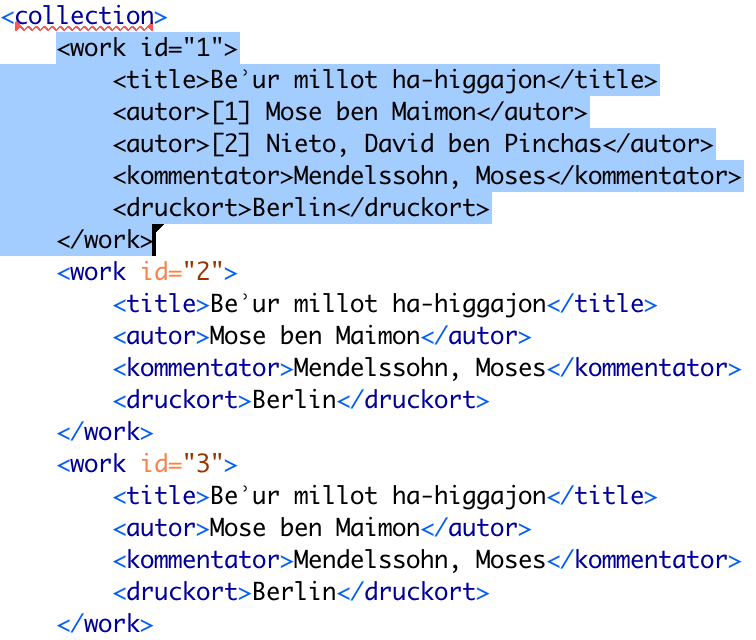
\includegraphics{./Bilder/kollatz-xml-Beispiel.png}
\caption{Auszug aus dem XML-Beispiel (Quelle: Kuczera)}
\end{figure}

Das root-Element in den XML-Beispiel ist . Innerhalb der collection finden sich Angaben zu verschiedenen Büchern, die jeweils wieder mit einem -Element zusammengefasst sind. Zu jedem Buch werden folgende Angaben gemacht:

\begin{itemize}
\tightlist
\item
  Titel des Buches im

  -Element
\item
  Autor(en) des Buches um -Element, ggf. durchnummeriert mit Zahlen in eckigen Klammern (z.B. {[}1{]})
\item
  Kommentator des Buches im -Element
\item
  Druckort des Buches im -Element
\end{itemize}

\section{Knotentypen}\label{knotentypen}

Für die Modellierung dieser Datenstruktur in der Graphdatenbank müssen zunächst die verschiedenen Entitäten identifiziert werden um festzulegen, welche Knotentypen notwendig sind. Als erstes scheint es sinnvoll einen Knoten vom Typ \texttt{Werk} anzulegen, wie es auch im XML über das -Element im XML modelliert ist. Die dem -Element untergeordneten Elemente

, , und sind für das Werk jeweils spezifisch. Den Titel eines Werkes können wir in einem \texttt{Titel}-Knoten ablegen, den Druckort in einem \texttt{Ortsknoten} und Autoren sowie Kommentatoren werden in \texttt{Personen}-Knoten gespeichert. Hier ist zu beachten das die identifizierten Entitäten, wie z.b. Personen nicht in Knotentypen gespeichert werden die ihre Rolle wieder geben (wie z.B. Autor oder Kommentator) sondern unabhängig von ihrer Rolle in allgemein gehaltenen Kategorien wie Person. Im Graphen werden die verschiedenen Rollen, wie Autor oder Kommentator dann über die Kanten modelliert, was im nächsten Abschnitt näher erläutert wird.

\section{Kantentypen}\label{kantentypen}

Nach den Knotentypen sind nun die Kantentypen festzulegen. Sie geben an, in welcher Beziehung die verschiedenen Knoten zueinander stehen. Sieht man sich die XML-Vorlage an, ergeben sich folgene Typen von Kanten:

\begin{itemize}
\tightlist
\item
  GEDRUCKT\_IN
\item
  AUTOR\_VON
\item
  KOMMENTIERT\_VON
\end{itemize}

Mit der \texttt{GEDRUCKT\_IN}-Kante werden ein Werk und ein Ort verbunden und damit angegeben, dass dieses Buch in jenem Ort gedruckt worden ist.

\begin{figure}
\centering
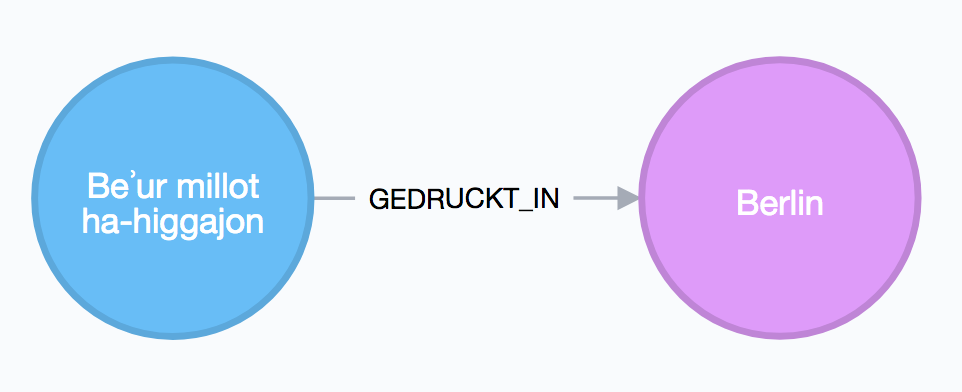
\includegraphics{Bilder/Werk-Ort.png}
\caption{Verbindung zwischen einem \texttt{Werk}- und einem \texttt{Ort}-Knoten (Quelle: Kuczera).}
\end{figure}

Die \texttt{AUTOR\_VON}-Kante verbindet einen Personenknoten mit einem Werkknoten und ordnet damit den Autor dem von ihm geschriebenen Buch zu.

\begin{figure}
\centering
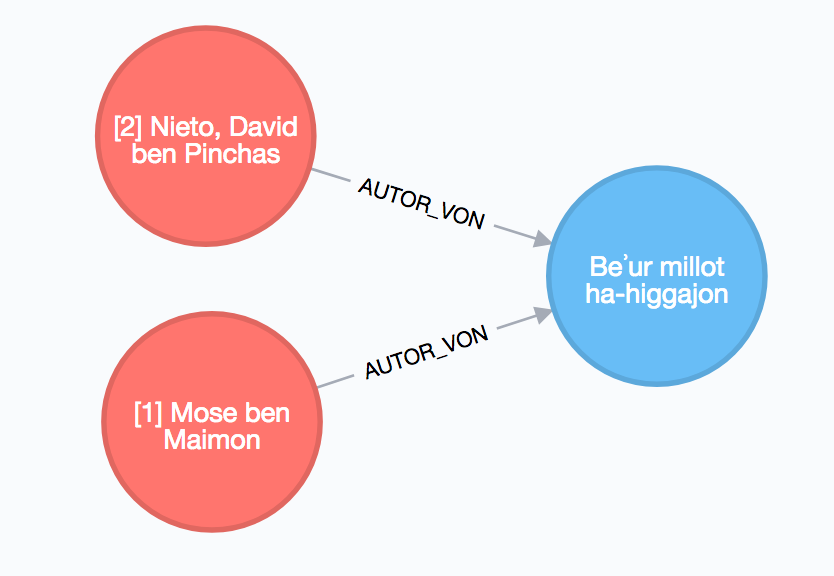
\includegraphics{Bilder/Werk-Autor.png}
\caption{Verbindung zwischen einem \texttt{Werk}- und einem \texttt{Ort}-Knoten (Quelle: Kuczera).}
\end{figure}

Mit der \texttt{KOMMENTIERT\_VON}-Kante wird auch ein Personenknoten einem Werkknoten zugeordnet, diesmal nimmt die Person aber die Rolle des Kommentierenden ein.

\begin{figure}
\centering
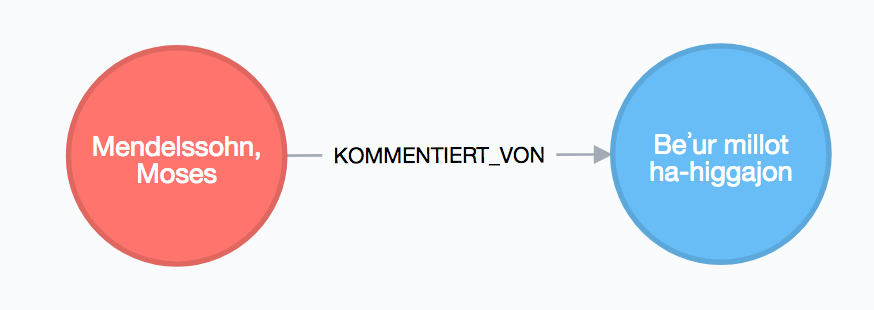
\includegraphics{Bilder/Werk-Kommentator.png}
\caption{Verbindung zwischen einem \texttt{Werk}- und einem \texttt{Ort}-Knoten (Quelle: Kuczera).}
\end{figure}

Im der folgenden Abbildung werden alle Knoten und Kanten des Beispiels gemeinsam dargestellt.

\begin{figure}
\centering
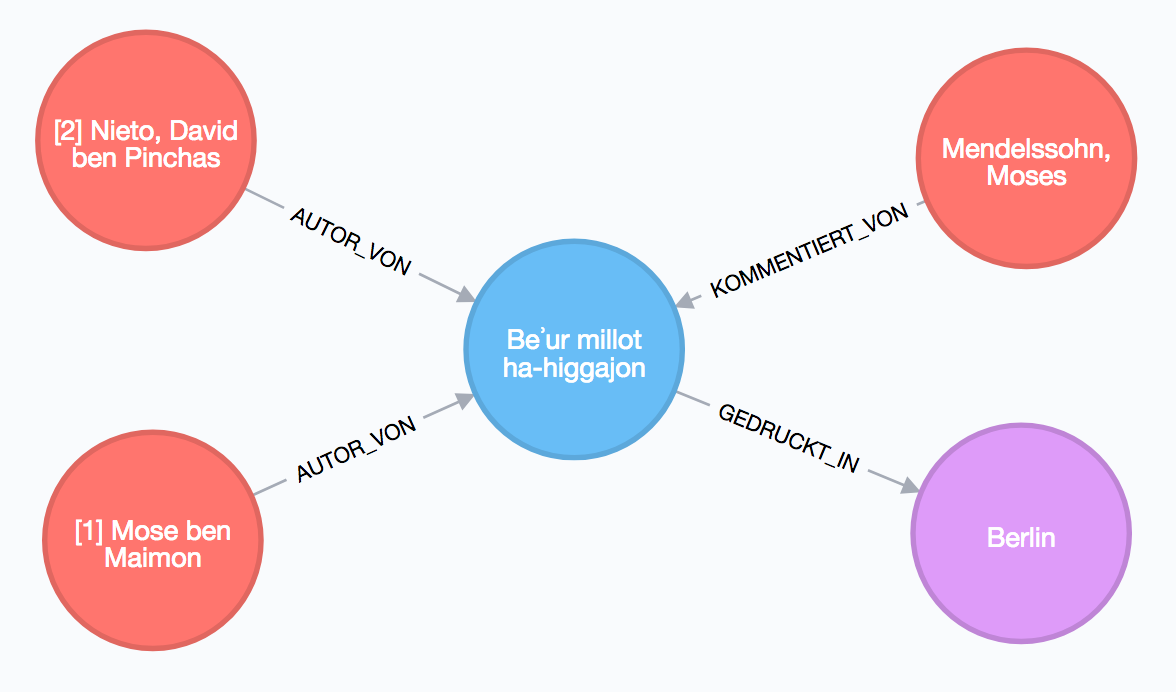
\includegraphics{Bilder/Werk-gesamt.png}
\caption{Verbindung zwischen einem \texttt{Werk}- und einem \texttt{Ort}-Knoten (Quelle: Kuczera).}
\end{figure}

Damit steht das Graphmodell fest und im nächsten Abschnitt geht es an den Import.

\section{Der Import mit apoc.load.xml}\label{der-import-mit-apoc.load.xml}

Für den Import von XML-Daten steht in der apoc-Bibliothek der Befehl apoc.load.xml zur Verfügung. Im folgenden wird zunächst der gesamte Befehl für den Import gelistet.

\begin{verbatim}
CALL apoc.load.xmlSimple("https://raw.githubusercontent.com/kuczera/Graphentechnologien/master/docs/data/kollatz.xml") yield value as xmlFile
UNWIND xmlFile._work as wdata
    MERGE (w1:Werk{eid:wdata.id})
    set w1.name=wdata._title._text
    FOREACH (name in wdata._autor |
        MERGE (p1:Person {Name:name._text})
        MERGE (p1)-[:AUTOR_VON]->(w1) )
    FOREACH (name in wdata._kommentator |
        MERGE (p1:Person {Name:name._text})
        MERGE (p1)-[:KOMMENTIERT_VON]->(w1))
    FOREACH (druckort in [x in
        wdata._druckort._text where x is not null] |
         MERGE (o1:Ort{name:druckort})
         MERGE (w1)-[:GEDRUCKT_IN]->(o1));
\end{verbatim}

Für den Import wird die apoc-Funktion apoc.load.xmlSimple verwendet\footnote{Die apoc-Bibliothek muss nach der Installation von neo4j zusätzlich installiert werden. Nähere Informationen zur Installation und die Dokumentation findet sich unter: \url{https://neo4j-contrib.github.io/neo4j-apoc-procedures/}. Die Dokumentation zu apoc.load.xml ist erreichbar unter \url{https://neo4j-contrib.github.io/neo4j-apoc-procedures/\#_load_xml}.}. Diese Funktion nimmt XML-Dateien oder eine URL und stellt die Daten geparst für die weitere Verarbeitung in einer Map-Struktur zur Verfügung (vgl. Zeile 1-4 des Codebeispiels). In der Variable \textbf{xmlFile} befindet sich nun diese Map-Struktur. In Zeile 5 folgt der \textbf{UNWIND}-Befehl, der jeweils ein Werk (das ist der Inhalt des \emph{work}-Elements in der XML-Datei) an die Variable value weitergibt, mit der es dann weiter verarbeitet werden kann. Dies wiederholt sich so lange, bis alle \emph{work}-Elemente der XML-Datei abgearbeitet sind.

Nach dem \texttt{UNWIND}-Befehl folgt als eine Gruppe von Befehlen, die immer wieder für jedes \emph{work}-Element ausgeführt werden. Als erstes wird mit dem \texttt{MERGE}-Befehl ein Knoten vom Typ \texttt{Werk}, für das Buch mit der Titelangabe in der Eigenschaft \texttt{name} erstellt. Dies ist nicht weiter schwierig, da in der XML-Datei für jedes Werk nur ein Titel existiert. Anders ist dies bei den Autoren, von denen einen oder mehrere geben kann, die dann auch in mehreren \emph{autor}-Elementen verzeichnet sind.

Die Funktion apoc.loadxmlSimple ist deprecated und wird von der Funktion apoc.loadxml abgelöst. Diese ist allgemeiner gültig aber dadurch in der Anwendung etwas komplizierter.

\begin{verbatim}
CALL
apoc.load.xml("https://raw.githubusercontent.com/kuczera/Graphentechnologien/master/docs/data/kollatz.xml", "/collection/*")  YIELD value AS work // this uses an xpath expression to get all child nodes of "<collection>""
WITH
[x in work._children where x._type="title" | x._text][0] as titel,
[x in work._children where x._type="autor" | x._text] as autoren,
[x in work._children where x._type="kommentator" | x._text] as kommentatoren,
[x in work._children where x._type="druckort" | x._text] as druckorte,
work.id as eid
MERGE (w:Werk{eid:eid})
SET w.name = titel
FOREACH (x in autoren |
   MERGE (p:Person {name:x})
   MERGE (p)-[:AUTOR_VON]->(w) )
FOREACH (x in kommentatoren |
   MERGE (p:Person {name:x})
   MERGE (w)-[:KOMMENTIERT_VON]->(p) )
FOREACH (x in druckorte |
   MERGE (o:Ort {name:x})
   MERGE (w)-[:GEDRUCKT_IN]->(o) );
\end{verbatim}

\chapter{Verwandtschaft im Graphen}\label{verwandtschaft-im-graphen}

In diesem Kapitel wird am Beispiel eines Ausschnitts der Daten des Projekts \textbf{Nomen et Gens}\footnote{Informationen zum Projekt „Nomen et Gens`` finden Sie unter \url{http://www.neg.uni-tuebingen.de/} (abgerufen am 10.08.2018).} die Modellierung von Verwandtschaft in der Graphdatenbank neo4j dargestellt.\footnote{Dieses Kapitel geht in großen Teilen zurück auf meinem Aufsatz Graphentechnologien in den Digitalen Geisteswissenschaften, in: ABI Technik 2017; 37(3): 179--196, \url{https://doi.org/10.1515/abitech-2017-0042}. URL: \url{https://www.degruyter.com/downloadpdf/j/abitech.2017.37.issue-3/abitech-2017-0042/abitech-2017-0042.pdf}, insbesondere die Seiten 179 bis 182 und wurde nur geringfügig ergänzt.}

\section{Das Projekt Nomen et Gens}\label{das-projekt-nomen-et-gens}

Das Projekt \textbf{Nomen et Gens} (NeG) zielt darauf ab, alle schriftlich belegten Namen und Personen Kontinentaleuropas in den vier Jahrhunderten vor Karl dem Großen (also von 400 bis 800 nach Christus) zu erfassen. Die Datenbank des Projekts geht auf ein erfolgreich abgeschlossenes DFG-Projekt zurück und wird aktuell von den Projektbeteiligten weiter betreut und sukzessive ausgebaut. Neben den Quellen der Personennennung, den unterschiedlichen Namensformen usw. werden auch die Verwandtschaftsbeziehungen zwischen identifizierten Personen in der Datenbank abgelegt. Dabei werden bis zu 16 verschiedene Verwandtschaftsbeziehungen in der Datenbank gespeichert, wie z. B. Bruder, Schwester, Sohn, Tochter, Vater, Mutter, Onkel oder Nichte. Bei einem Personendatensatz werden dann jeweils die Verwandtschaftsbeziehungen aufgelistet, so dass man sich ggf. jeweils von Person zu Person durchklicken muss, bis man am Ziel angelangt ist.

\section{Nomen et Gens im Graphen}\label{nomen-et-gens-im-graphen}

Vor diesem Hintergrund bot es sich an, die Personen und die zugehörigen Verwandtschaftsbeziehungen in die Graphdatenbank neo4j zu transferieren und anschließend graphbasierte Abfrageperspektiven zu testen.

\begin{figure}
\centering
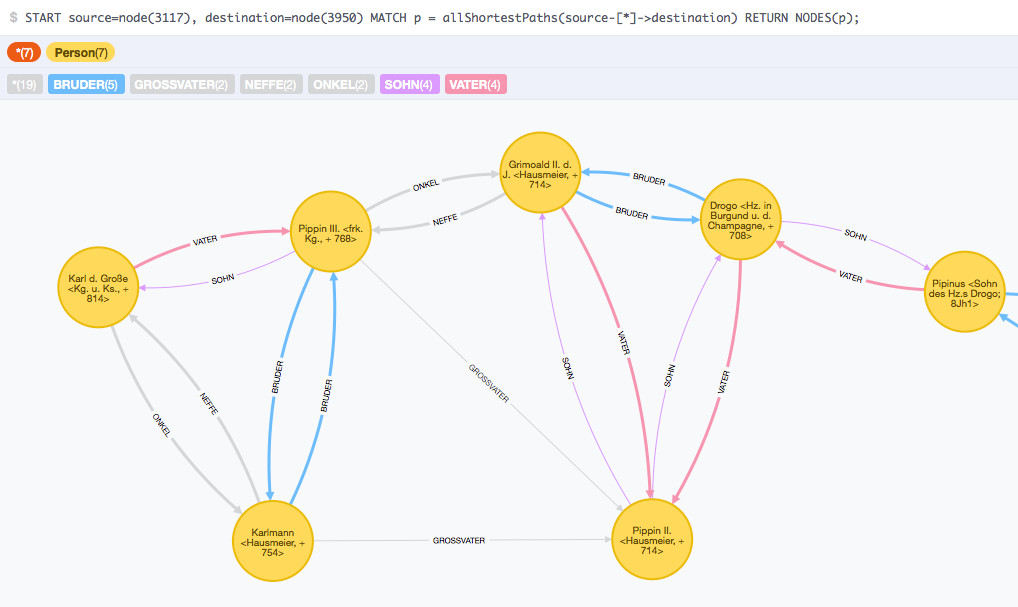
\includegraphics{Bilder/NeG/020-Verwandschaften.jpg}
\caption{Erste Importergebnisse}
\end{figure}

Die Abbildung zeigt die ersten Ergebnisse des Datenbankimports. Aus der Visualisierung werden die zahlreichen redundanten Beziehungen deutlich, die in der Folge zu neuen Modellierungsansätzen für die Verwandtschaftsbeziehungen führten. Ergebnis der Überlegungen war die Reduzierung der möglichen Verwandtschaftsbeziehungen auf die zwei Kantentypen \texttt{KIND} und \texttt{VERHEIRATET\_MIT}. Dabei wird eine Kante vom Typ \texttt{KIND} für eine Eltern-Kind-Beziehung nur einmal vergeben, während eine Kante vom Typ \texttt{VERHEIRATET\_MIT} immer zweifach in jeweils umgekehrter Richtung angelegt wird. Dies ergibt sich aus der Überlegung, dass eine Eltern-Kind-Beziehung gerichtet ist und zwar in unserem Fall vom Elternteil zum Kind hin, während eine \texttt{VERHEIRATET\_MIT}-Beziehung ungerichtet ist: Wenn eine Person mit einer anderen Person verheiratet ist, ist die andere Personen automatisch auch mit der ersten verheiratet. Da im Property-Graph-Modell von neo4j jede Kante genau eine Richtung haben muss, wird die \texttt{VERHEIRATET\_MIT}-Kante zweimal in jeweils unterschiedliche Richtung angelegt, während bei der hierarchischen Eltern-Kind-Beziehung eine Kante ausreicht.

\begin{figure}
\centering
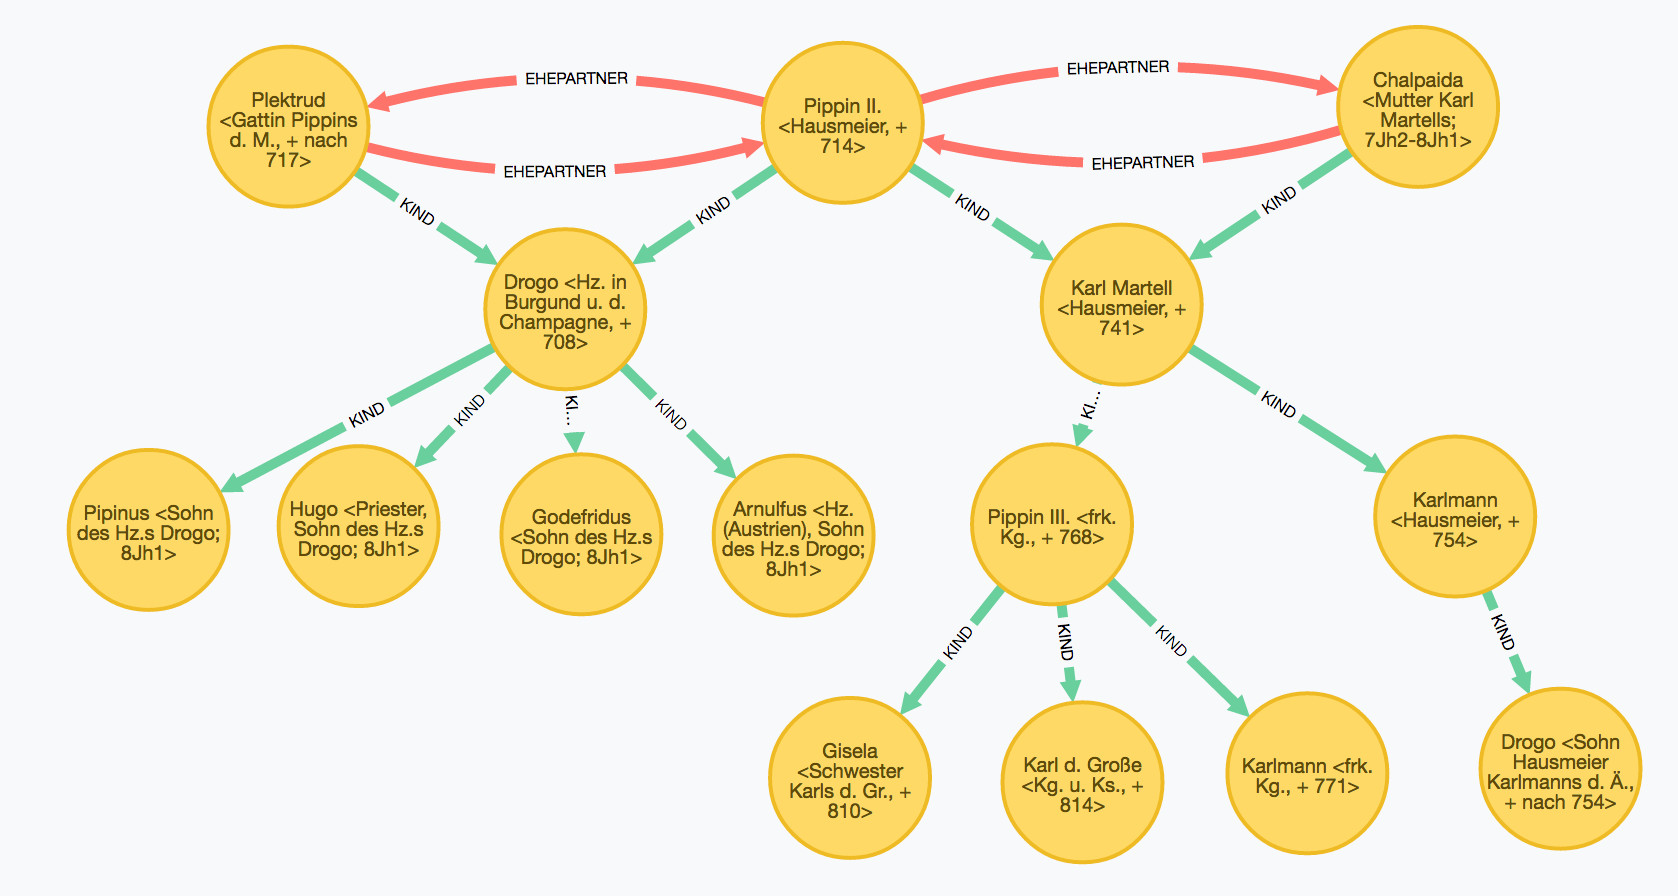
\includegraphics{Bilder/NeG/030-Urenkel-Pippins.jpg}
\caption{Die Urenkel Pippins}
\end{figure}

\section{Sind Berchar und Karl der Große verwandt ?}\label{sind-berchar-und-karl-der-grouxdfe-verwandt}

Im folgenden Beispiel soll das Potential der Graphmodellierung von Verwandtschaftsbeziehungen demonstriert werden. In der Datenbank gibt es die Person Berchar. Berchar war ein Hausmeier König Theuderichs III. Die Frage ist nun, ob dieser Berchar mit Karl dem Großen verwandt ist. In der NeG-Datenbank ist ein Verwandtschaftsverhältnis von Berchar zu Karl dem Großen nicht direkt ableitbar.

\begin{figure}
\centering
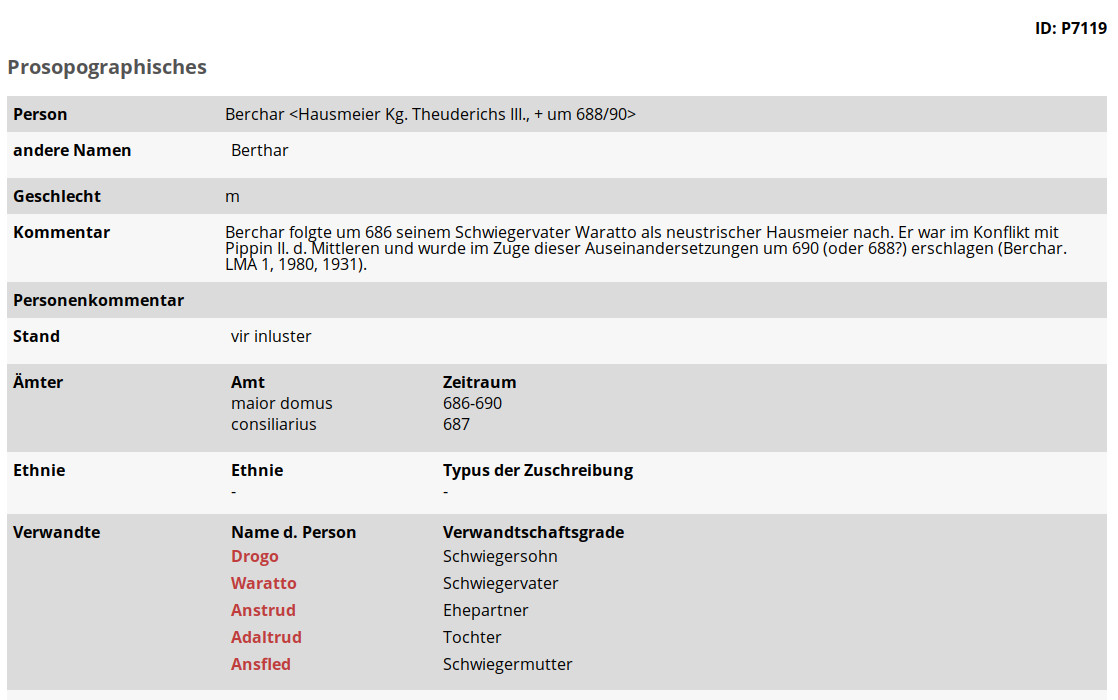
\includegraphics{Bilder/NeG/040-Berchar-DB-Eintrag.jpg}
\caption{Berchar in der Nomen-et-Gens-Datenbank}
\end{figure}

In der Graphdatenbank neo4j wird für eine solche Fragestellung eine Shortest\_Path-Abfrage verwendet, die den kürzesten möglichen Weg zwischen zwei Knoten zurück liefert, sofern es einen gibt. Der folgende cypher-Befehl liefert den Pfad zwischen dem Personenknoten Karls des Großen mit der NeG-ID 7404 und dem Personenknoten von Berchar mit der NeG-ID 7119. Dabei wird die Länge des abzufragenden Pfades auf 15 Kanten begrenzt.

\begin{verbatim}
// shortest_path-Abfrage von Karl dem Großen zu Berchar
MATCH (KdG:Person { nid:'7404' })
MATCH (Berchar:Person { nid:'7119' })
p = shortestPath((KdG)-[*..15]-(Berchar))
RETURN p;
\end{verbatim}

Das Ergebnis zeigt, dass Berchar tatsächlich mit Karl dem Großen verwandt ist. Er ist nämlich der Schwiegervater von Drogo (Herzog in Burgund und der Champagne, gest. 708), der wiederum der Bruder des Großvaters Karls des Großen ist.

\begin{figure}
\centering
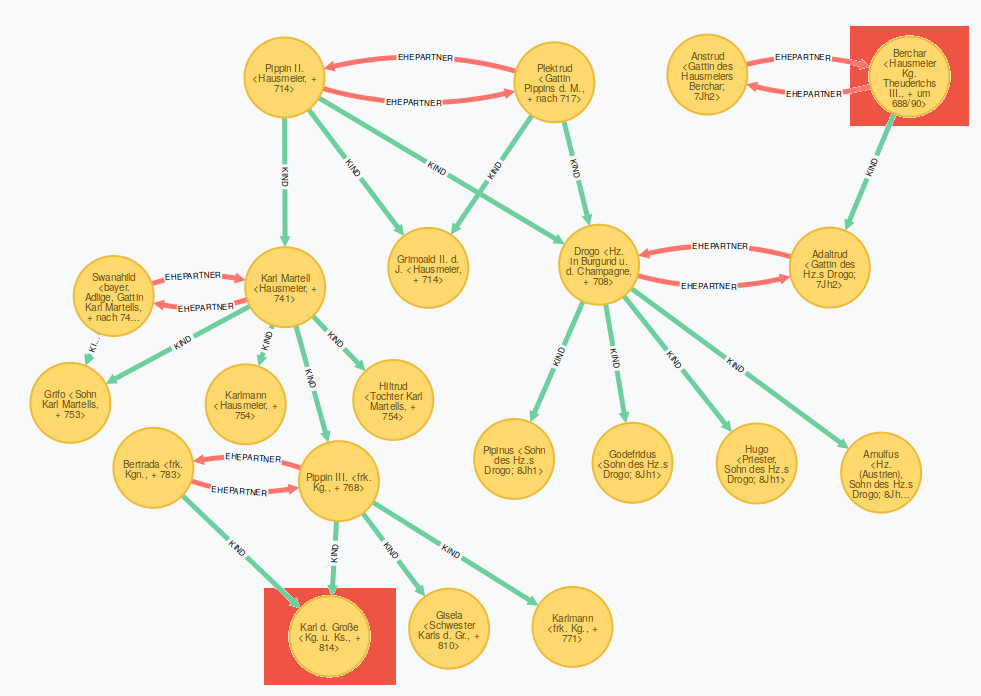
\includegraphics{Bilder/NeG/050-Berchar-Karl-shortestpath.jpg}
\caption{Der kürzeste Pfad (shortestPath) von Karl zu Berchar.}
\end{figure}

\section{Zusammenfassung}\label{zusammenfassung-2}

Mit diesem Beispiel sind die interessanten Erschließungs- und Modellierungsperspektiven für die digitale Genealogie nur angedeutet. Mit Graphentechnologien lässt sich intuitive Datenmodellierung mit sehr flexiblen Erschließungs- und Abfragemöglichkeiten kombinieren.

\chapter{Das DTA im Graphen}\label{das-dta-im-graphen}

Das Deutsche Textarchiv (DTA) stellt einen Disziplinen übergreifenden Grundbestand deutscher Werke aus dem Zeitraum von ca. 1600 bis 1900 im Volltext und als digitale Faksimiles frei zur Verfügung und bereitet ihn so auf, dass er über das Internet in vielfältiger Weise nutzbar ist. Das DTA-Korpus soll in größtmöglicher Breite widerspiegeln, was an bedeutenden Werken in deutscher Sprache veröffentlicht wurde. Die ausgewählten Texte stehen repräsentativ für die Entwicklung der deutschen Sprache seit der Frühen Neuzeit. Alle DTA-Texte werden unter einer offenen Lizenz veröffentlicht (CC BY-NC). Das DTA fördert die Wiederverwendung seiner Texte in allen Bereichen der Digitalen Geisteswissenschaften.

\section{Die Downloadformate des DTA}\label{die-downloadformate-des-dta}

Das DTA bietet zu den bereitgestellten Texten verschiedene Formate zum Download an. Als Beispiel wird hier \href{http://deutschestextarchiv.de/book/show/goethe_faust01_1808}{Goethes Faust} in der ersten Auflage von 1808 importiert.

\begin{itemize}
\tightlist
\item
  \href{http://deutschestextarchiv.de/book/download_xml/goethe_faust01_1808}{TEI-P5} bietet die textkritische Fassung des Faust
\item
  \href{http://deutschestextarchiv.de/book/download_fulltcf/16181}{TCF} bietet die tokenisierte, serialisierte, lemmatisierte und normalisierte Fassung, textkritische Informationen fehlen jedoch.
\item
  \href{http://deutschestextarchiv.de/book/download_txt/goethe_faust01_1808}{Plain-Text} bietet einen einfachen Text mit Seiten- und Zeilenfall ohne weitere Zusatzinformationen
\end{itemize}

Für den Import in eine Graphdatenbanken bietet sich das TCF-Format an, da es den Text tokenisiert, serialisiert, lemmatisiert und normalisiert bietet. In diesem Format lässt er sich mit cypher-Befehlen in die Graphdatenbank importieren. Im Beispiel wird Goethes Faust in der TCF-Fassung in die Graphdatenbank importiert.

Hier wird ein Ausschnitt aus der TCF-Datei\footnote{Vgl. zu diesem Beispiel \url{http://deutschestextarchiv.de/book/view/goethe_faust01_1808?p=11}.} gezeigt

\begin{Shaded}
\begin{Highlighting}[]
\KeywordTok{<token}\OtherTok{ ID=}\StringTok{"w5b"}\KeywordTok{>}\NormalTok{Ihr}\KeywordTok{</token>}
\KeywordTok{<token}\OtherTok{ ID=}\StringTok{"w5c"}\KeywordTok{>}\NormalTok{bringt}\KeywordTok{</token>}
\KeywordTok{<token}\OtherTok{ ID=}\StringTok{"w5d"}\KeywordTok{>}\NormalTok{mit}\KeywordTok{</token>}
\KeywordTok{<token}\OtherTok{ ID=}\StringTok{"w5e"}\KeywordTok{>}\NormalTok{euch}\KeywordTok{</token>}
\KeywordTok{<token}\OtherTok{ ID=}\StringTok{"w5f"}\KeywordTok{>}\NormalTok{die}\KeywordTok{</token>}
\KeywordTok{<token}\OtherTok{ ID=}\StringTok{"w60"}\KeywordTok{>}\NormalTok{Bilder}\KeywordTok{</token>}
\KeywordTok{<token}\OtherTok{ ID=}\StringTok{"w61"}\KeywordTok{>}\NormalTok{froher}\KeywordTok{</token>}
\KeywordTok{<token}\OtherTok{ ID=}\StringTok{"w62"}\KeywordTok{>}\NormalTok{Tage}\KeywordTok{</token>}
\KeywordTok{<token}\OtherTok{ ID=}\StringTok{"w63"}\KeywordTok{>}\NormalTok{,}\KeywordTok{</token>}
\KeywordTok{<token}\OtherTok{ ID=}\StringTok{"w64"}\KeywordTok{>}\NormalTok{Und}\KeywordTok{</token>}
\KeywordTok{<token}\OtherTok{ ID=}\StringTok{"w65"}\KeywordTok{>}\NormalTok{manche}\KeywordTok{</token>}
\KeywordTok{<token}\OtherTok{ ID=}\StringTok{"w66"}\KeywordTok{>}\NormalTok{liebe}\KeywordTok{</token>}
\KeywordTok{<token}\OtherTok{ ID=}\StringTok{"w67"}\KeywordTok{>}\NormalTok{Schatten}\KeywordTok{</token>}
\end{Highlighting}
\end{Shaded}

und im Anschluss im Vergleich das Original (links) und der Lesetext (rechts).

\begin{figure}
\centering
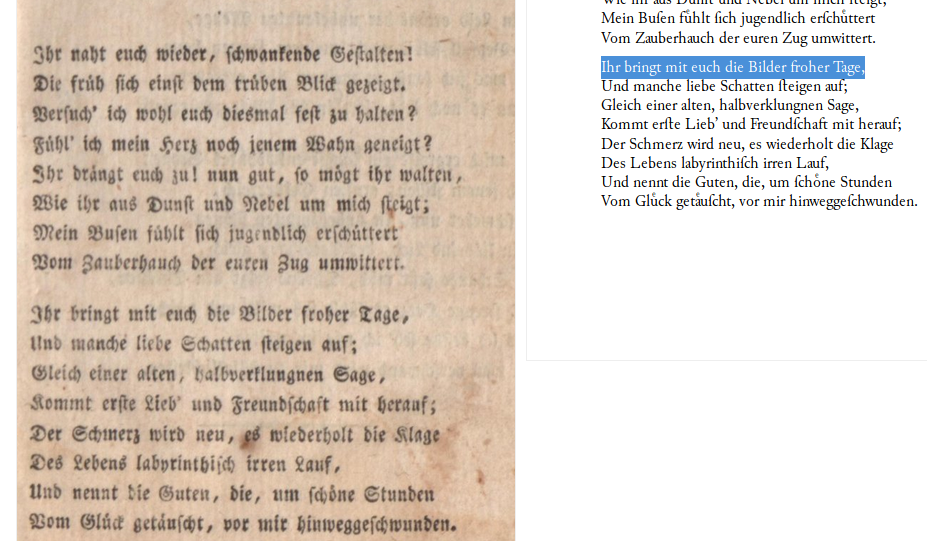
\includegraphics{Bilder/Faust-S11-Faks.png}
\caption{Eine Beispielzeile aus dem Faust}
\end{figure}

Vergleicht man das TCF-Xml mit der gleiche Stelle im TEIP5 ist zu erkennen, dass in letzterem der Zeilenfall annotiert ist.

\begin{Shaded}
\begin{Highlighting}[]
\KeywordTok{<lb/>}
  \KeywordTok{<lg}\OtherTok{ n=}\StringTok{"2"}\KeywordTok{>}
      \KeywordTok{<l>}\NormalTok{Ihr bringt mit euch die Bilder froher Tage,}\KeywordTok{</l><lb/>}
      \KeywordTok{<l>}\NormalTok{Und manche liebe Schatten }\DecValTok{&#x017F;}\NormalTok{teigen auf;}\KeywordTok{</l><lb/>}
\end{Highlighting}
\end{Shaded}

Die Downloadformate sind also für verschiedene Nutzungsszenarien optimiert. Für den Import in eine Graphdatenbank bietet sich das TCF-Format an.

\section{Vorbereitungen}\label{vorbereitungen}

Als Vorbereitung müssen einige Constraints eingerichtet werden.\footnote{Zu \textbf{constraints} vgl. \url{https://neo4j.com/docs/developer-manual/current/cypher/schema/constraints/}}

\begin{verbatim}
create constraint on (t:Token) assert t.id is unique;
create constraint on (s:Sentence) assert s.id is unique;
create constraint on (l:Lemma) assert l.text is unique;
\end{verbatim}

Mit den Befehlen wird sichergestellt, dass die im nächsten Schritt importierten Knoten eindeutige IDs haben.

\section{Import des TCF-Formats}\label{import-des-tcf-formats}

\subsection{Tokenimport}\label{tokenimport}

Nun folgt der Import-Befehl mit der apoc-procedure \emph{apoc.load.xmlSimple}.

\begin{verbatim}
call apoc.load.xml('http://deutschestextarchiv.de/book/download_fulltcf/16181') yield value as doc
unwind doc._TextCorpus._tokens._token as token
create (t:Token{id:token.ID, text:token._text})
with collect(t) as tokens
unwind apoc.coll.pairs(tokens)[0..-1] as value
with value[0] as a, value[1] as b
create (a)-[:NEXT_TOKEN]->(b);
\end{verbatim}

In der ersten Zeile wird der apoc-Befehl \emph{apoc.load.xmlSimple} aufgerufen, der als Argument die URL der TCF-Version von Goethes Faust im Deutschen Textarchiv erhält. Die weiteren cypher-Befehle parsen die XML-Datei und spielen die Token (also die einzelnen Wörter) als Wortknoten in die Graphdatenbank ein. Schließlich werden die NEXT\_TOKEN-Kanten zwischen den eingespielten Wörtern erstellt.

\subsection{Satzstrukturen}\label{satzstrukturen}

Der nächste Befehl lädt wieder die gleiche XML-Datei und importiert die Satzstrukturen.

\begin{verbatim}
call apoc.load.xmlSimple("http://deutschestextarchiv.de/book/download_fulltcf/16181") yield value as doc
unwind doc._TextCorpus._sentences._sentence as sentence
match (t1:Token{id:head(split(sentence.tokenIDs, " "))})
match (t2:Token{id:last(split(sentence.tokenIDs, " "))})
create (s:Sentence{id:sentence.ID})
create (s)-[:SENTENCE_STARTS]->(t1)
create (s)-[:SENTENCE_ENDS]->(t2)
with collect(s) as sentences
unwind apoc.coll.pairs(sentences)[0..-1] as value
with value[0] as a, value[1] as b
create (a)-[:NEXT_SENTENCE]->(b);
\end{verbatim}

\subsection{Lemmaimport}\label{lemmaimport}

Im folgenden Befehl werden die Lemmata importiert und jedes Token mit dem zugehörigen Lemma verknüpft.

\begin{verbatim}
call apoc.load.xmlSimple('http://deutschestextarchiv.de/book/download_fulltcf/16181') yield value as doc
unwind doc._TextCorpus._lemmas._lemma as lemma
match (t:Token{id:lemma.tokenIDs})
merge (l:Lemma{text:lemma._text})
create (t)-[:LEMMATISIERT]->(l);
\end{verbatim}

Der letzte Befehl ergänzt bei jedem Token-Knoten noch die Lemma-Information als Proptery.

\begin{verbatim}
call apoc.load.xmlSimple('http://deutschestextarchiv.de/book/download_fulltcf/16181') yield value as doc
unwind doc._TextCorpus._lemmas._lemma as lemma
match (t:Token{id:lemma.tokenIDs}) set t.Lemma = lemma._text;
\end{verbatim}

Damit ist nun die Fassung von Goethes Faust aus dem Deutschen Textarchiv in die Graphdatenbank importiert worden und kann weiter untersucht werden (hier klicken, um den Code mit den cypher-Querys für den gesamten Artikel herunterzuladen).

\subsection{Beispielabfrage}\label{beispielabfrage}

Bei Cypher-Abfragen können alle Eigenschaften von Knoten und Kanten miteinbezogen werden. Der Query fragt nach einem \texttt{Token}-Knoten mit dem Lemma \textbf{Bild}, gefolgt von einem \texttt{Token}-Knoten mit dem Lemma \textbf{froh} und dazu die drei vorhergehenden und die drei nachfolgenen \texttt{Token}-Knoten.

\begin{verbatim}
MATCH
w=()-[:NEXT_TOKEN*5]->(a:Token{Lemma:'Bild'})
-[:NEXT_TOKEN]->(b:Token{Lemma:'froh'})
-[:NEXT_TOKEN*5]->()
RETURN *;
\end{verbatim}

Damit finden wir die am Anfang des Kapitels vorgestellte Stelle im Graphen

\begin{figure}
\centering
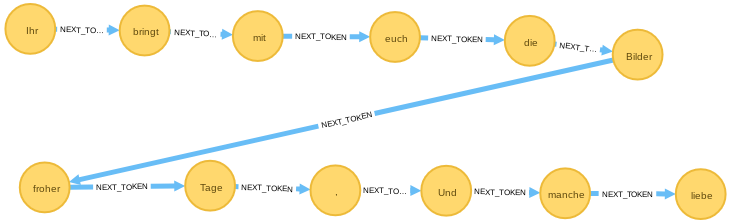
\includegraphics{Bilder/TEI2Graph/BilderFroherTage.png}
\caption{Eine Beispielzeile aus dem Faust}
\end{figure}

\section{Import der TEIP5-Fassung}\label{import-der-teip5-fassung}

Im nächsten Schritt wird die TEIP5-Fassung von Goethes Faust importiert

\begin{verbatim}
call
apoc.xml.import("http://deutschestextarchiv.de/book/download_xml/goethe_faust01_1808",{createNextWordRelationships:
true})
yield node
return node;
\end{verbatim}

und mit dem folgenden Query auch jene \textbf{Bilder froher Tage}-Stelle im Text aufgerufen.

\begin{verbatim}
MATCH
w=(:XmlWord)-[:NEXT_WORD*3]->
(a:XmlWord {text:'Bilder'})-[:NEXT_WORD]->
(:XmlWord {text:'froher'})-[:NEXT_WORD*3]->(:XmlWord)
RETURN *;
\end{verbatim}

Das Ergebnis zeigt die komplexere Struktur der gleichen Stelle im TEIP5-Graphen, da hier u.a. auch der Zeilenfall annotiert ist.

\begin{figure}
\centering
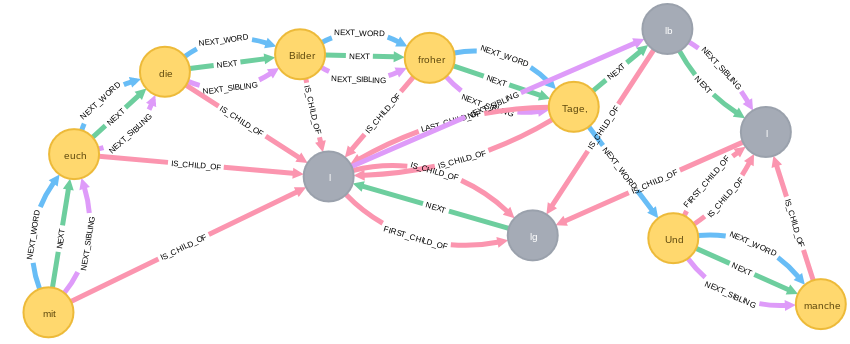
\includegraphics{Bilder/TEI2Graph/BilderFroherTageP5.png}
\caption{Die Beispielzeile aus der TEIP5-Fassung des Faust}
\end{figure}

\section{Zusammenfassung}\label{zusammenfassung-3}

Im vorliegenden Kapitel wurden die Schritte für den Import der DTA-TCF-Fassung von Goethes Faust in die Graphdatenbank neo4j vorgestellt. Die qualitativ hochwertigen Text-Quellen des Deutschen Textarchivs bieten in Verbindung mit Graphdatenbanken sehr interessante neue Möglichkeiten zur Auswertung der Texte. Durch Austausch des Links zur TCF-Fassung können auch andere Texte des DTA eingespielt werden. Am Ende wurde beispielhaft die TEI-P5-Fassung eingespielt um die gleiche Stelle in beiden Fassungen vergleichen zu können. Weitere Informationen zu XML im Graphen finden Sie im Kapitel zu \href{https://kuczera.github.io/Graphentechnologien/60_XML-Text-im-Graphen.html}{XML-Text im Graphen}.

\chapter{Textmodelle im Graphen}\label{textmodelle-im-graphen}

\section{Text als Graph}\label{text-als-graph}

Die Diskussion über Modellierungsansätze von Text als Graph hält aktuell an.\footnote{Vgl. zuletzt @DekkerHaentjensItmorejust2017.}

\subsection{XML-Dateien als Ketten von Zeichen}\label{xml-dateien-als-ketten-von-zeichen}

Da die technische Grundlage von XML Textdateien sind, handelt es sich bei XML um eine eindimensionale Kette von Tokens\footnote{@HuitfeldtMarkupTechnologyTextual2014, S. 161 sieht digitale Dokumente prinzipiell als lineare Sequenz von Zeichen}.

\subsection{Modellierungsüberlegungen}\label{modellierungsuxfcberlegungen}

Prinzipiell können XML-Dateien ohne größere Probleme in einen Graphen importiert werden, da sie einen geerdeten, gerichteten azyklischen Graphen, der vielfache Elternbeziehungen verhindert, und damit ein Ordered Hierarchy of Content Objects (OHCO) darstellen. Es gibt vor allem im Bereich des Mixed-Content verschiedene Ansätze, XML-Strukturen im Graphen abzubilden\footnote{Vgl. @DekkerHaentjensItmorejust2017.}. Überlegungen zur Auslagerung von Annotationen aus XML in eine Graphdatenbank brachte schon Desmond Schmidt in die Diskussion ein:

\emph{Embedded annotations can also be removed from TEI texts. The elements \texttt{\textless{}note\textgreater{}}, \texttt{\textless{}interp\textgreater{}}, and \texttt{\textless{}interpGrp\textgreater{}} describe content that, like metadata, is about the text, not the text itself. These are really annotations, and should ideally be represented via the established standards and practices of external annotation (Hunter and Gerber 2012). Annotations are stored in triple stores or graph databases like Neo4J,20 which record the identifiers of each component of the annotation and its data}\footnote{@SchmidtInteroperableDigitalScholarly2014, 4.1 Annotations.}.

\subsubsection{Granularität des Modells -- Was ist ein Token ?}\label{granularituxe4t-des-modells-was-ist-ein-token}

Für den Bereich der historisch-kritischen und philologischen Editionen ist es in der Regel ausreichend, beim Import von XML-kodierten Texten in den Graphen jeweils ein Wort in einen Knoten zu importieren, da meist die historische Aussage der Quelle im Vordergrund steht. In anderen Bereichen der digitalen Geisteswissenschaften kann die Entscheidung, welche Einheit für den Import in einen Knoten gewählt wird, durchaus anders ausfallen. So ist für Philologien die Betrachtung auf Buchstabenebene interessant\footnote{In FuD (http://fud.uni-trier.de/) werden Texte in Standoff-Markup auf Buchstabenebene ausgezeichnet, während beim DTA-Basisformat der Fokus auf der wortbasierten Auszeichung liegt (vgl. http://www.deutschestextarchiv.de/doku/basisformat/eeAllg.html).}. Im Graphmodell ist man im Hinblick auf die Granularität des Datenmodells wesentlich flexibler als z.B. bei XML oder Standoff-Markup. So ist es beispielsweise denkbar, an einen Wortknoten eine weitere Kette von Knoten anzulagern, welche pro Knoten jeweils einen Buchstaben des Wortes und die zugehörigen Annotationen enthalten. Es handelt sich um einen buchstabenbasierten Sub-Graphen, dessen Anfang und Ende mit dem Wortknoten verbunden ist. Damit können verschiedene Granularitätsstufen in einem Modell und in einer Datenbank abgebildet werden.

\begin{figure}
\centering
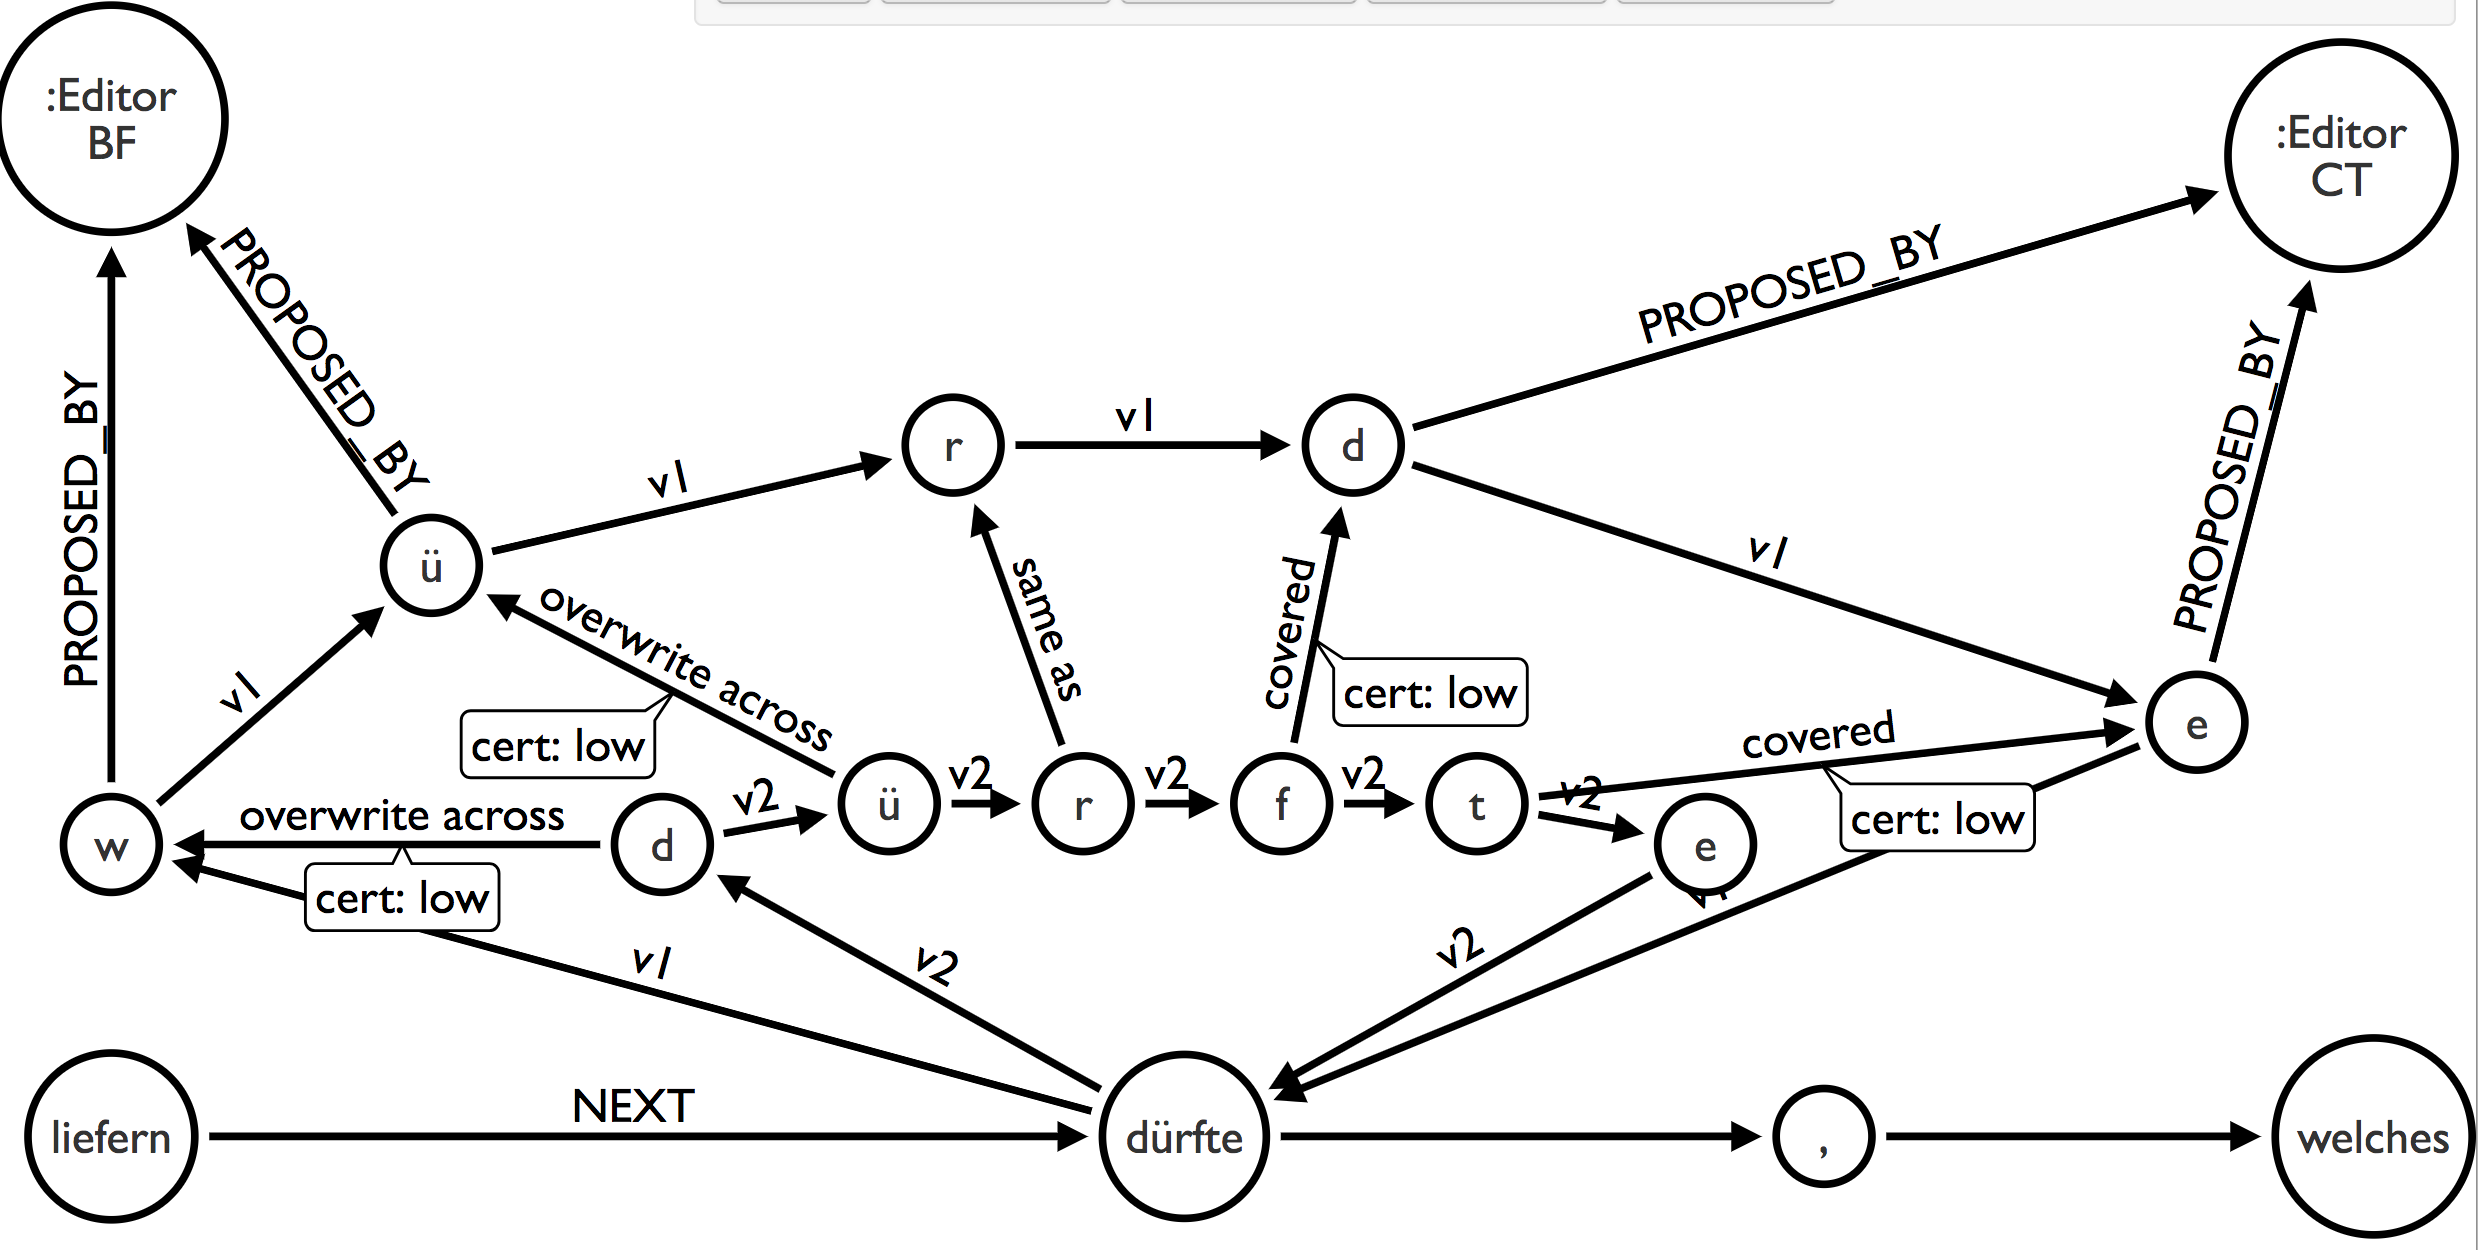
\includegraphics{Bilder/Granularitaet-im-Graphen.png}
\caption{Granularität von Text im Graphen}
\end{figure}

\section{Technische Vorbemerkungen}\label{technische-vorbemerkungen}

\subsection{Die Graphdatenbank neo4j}\label{die-graphdatenbank-neo4j}

Technische Grundlage der im Rahmen dieses Werkes vorgestellten Beispiel ist die Graphdatenbank neo4j\footnote{Vgl. www.neo4j.com (abgerufen am 7.8.2017).}. Die Graphdatenbank gibt es unter Open-Source-Lizenz in einer Community-Edition und unter einer kommerziellen Lizenz in einer Enterprise-Edition. Für die hier vorliegenden Aufgabengebiete war die Leistungsfähigkeit der Community-Edition völlig ausreichend. Darüber hinaus hat sich neo4j in den letzten Jahren als eine der führenden Graphdatenbanken etabliert und bietet neben stabiler Funktionalität auch genormte Schnittstellen. Prinzipiell wurde darauf hingearbeitet, dass die hier vorgestellten Überlegungen zu Graphenmodellierung historisch-kritischer Editionen auch auf andere Property-Graphdatenbanken wie z.b. orientdb\footnote{Die Graphdatenbank orientdb (http://orientdb.com/) bietet ein für Historiker sehr interessantes Feature, da sie als Datentyp für die Propertys von Knoten auch Datumsangaben im ISO-Format zulässt. Vgl. https://orientdb.com/docs/2.2/Managing-Dates.html (abgerufen am 7.8.2017).} übertragbar sind.

\subsection{Der neo4j-XML-Importer}\label{der-neo4j-xml-importer}

Für den Import der Texte wurde die Procedure apoc.xml.import aus der apoc-Bibliothek von neo4j verwendet\footnote{Wie die apoc-Bibliothek installiert und die Funktionen und Procedures verwendet werden können wird im \href{85-cypher-fuer-Fortgeschrittene.md}{Kapitel für Fortgeschrittene} erklärt.}. Die Procedure nimmt XML-Dateien entgegen und importiert sie in die Graphdatenbank.

\subsubsection{Import}\label{import}

Befehl für den Import der Patzig-XML-Datei\footnote{Für die Vereinheitlichung des Druckbildes mussten an einigen Stellen Zeilenumbrüche in die Codebeispiele eingefügt werden, die deren direkte Ausführung behindern.}:

\begin{verbatim}
CALL apoc.xml.import('http://www.deutschestextarchiv.de/
    book/download_xml/patzig_msgermfol841842_1828',
    {createNextWordRelationships: true})    
    yield node return node;
\end{verbatim}

Dabei werden die XML-Knoten in Graphknoten umgewandelt und verschiedene Arten von Kanten erstellt, die einerseits die Baum-Hierarchie des XMLs im Graphen abbilden. Mit der Option \texttt{createNextWorkRelationships:\ true} wird darüber hinaus festgelegt, dass die im XML vorhandenen Textknoten über \texttt{NEXT\_WORD}-Kanten miteinerander verknüpft werden. Zu beachten ist hierbei, dass es in TEI-XML zwei verschiedene Arten von Elementen gibt. Die eine Klasse dient der Klassifizierung von Text, die zweite Art bringt Varianten und zusätzlichen Text mit, der beim Import in seiner Serialität eingelesen und mit \texttt{NEXT\_WORD}-Kanten verbunden wird. Dies kann dann zur Sinnentstellung des Textes führen.\footnote{!!! Literaturhinweis ergänzen, Hans-Werner Bartz fragen.}

Zur Abbildung des Wurzelelement der importieren XML-Datei wird ein Knoten vom Typ \texttt{XmlDocument} angelegt. Dieser erhält die Propertys \texttt{\_xmlEncoding} zur Darstellung des Encodings, \texttt{\_xmlVersion} für die Xml-Version und \texttt{url} für die URL des importierten XML-Dokuments.

Mit einem weiteren cypher-Query erhalten alle der importierten Knoten die Eigenschaft \texttt{url} mit der URL des importierten XML-Dokuments. Damit lassen sich Knoten in einer Graphdatenbank mit mehreren importierten XML-Dokumenten auseinanderhalten.

\begin{verbatim}
MATCH (d:XmlDocument)-[:NEXT_WORD*]->(w:XmlWord)
SET w.url = d.url;
\end{verbatim}

Mit dem nächsten cypher-Query werden die Knoten des importierten XML-Dokuments durchnummertiert und der jeweilige Wert in der Property \texttt{DtaID} abgelegt.

\begin{verbatim}
MATCH p = (start:XmlDocument)-[:NEXT*]->(end:XmlTag)
WHERE NOT (end)-[:NEXT]->() AND start.url =  'http://www.deutschestextarchiv.de/book/download_xml/patzig_msgermfol841842_1828'
WITH nodes(p) as nodes, range(0, size(nodes(p))) AS indexes
UNWIND indexes AS index
SET (nodes[index]).DtaID = index;
\end{verbatim}

\subsubsection{Erläuterung der entstandenen Graphstrukturen}\label{erluxe4uterung-der-entstandenen-graphstrukturen}

Nach Abschluss des Imports werden jetzt die importierten Datenstrukturen erläutert. In der folgenden Tabelle werden die verschiedenen Typen von Knoten erläutert, die während des Imports erstellt wurden.

Tabelle zum Importvorgang der XML-Elemente und den entsprechenden Knoten

\begin{longtable}[]{@{}lll@{}}
\toprule
\begin{minipage}[b]{0.24\columnwidth}\raggedright\strut
XML-Knoten\strut
\end{minipage} & \begin{minipage}[b]{0.23\columnwidth}\raggedright\strut
Graphknoten\strut
\end{minipage} & \begin{minipage}[b]{0.44\columnwidth}\raggedright\strut
Bemerkungen\strut
\end{minipage}\tabularnewline
\midrule
\endhead
\begin{minipage}[t]{0.24\columnwidth}\raggedright\strut
XML-Wurzelelement\strut
\end{minipage} & \begin{minipage}[t]{0.23\columnwidth}\raggedright\strut
XmlDocument\strut
\end{minipage} & \begin{minipage}[t]{0.44\columnwidth}\raggedright\strut
Gibt es nur einmal. Es enthält Angaben zur Encodierung, zur XML-Version und die URL der importierten XML-Datei\strut
\end{minipage}\tabularnewline
\begin{minipage}[t]{0.24\columnwidth}\raggedright\strut
XML-Element-Knoten\strut
\end{minipage} & \begin{minipage}[t]{0.23\columnwidth}\raggedright\strut
XmlTag-Knoten\strut
\end{minipage} & \begin{minipage}[t]{0.44\columnwidth}\raggedright\strut
Die Attribute des XML-Elements werden in entsprechende Propertys des XMLTag-Knotens in der Datenbank umgewandelt\strut
\end{minipage}\tabularnewline
\begin{minipage}[t]{0.24\columnwidth}\raggedright\strut
XML-Text-Knoten\strut
\end{minipage} & \begin{minipage}[t]{0.23\columnwidth}\raggedright\strut
XmlWord\strut
\end{minipage} & \begin{minipage}[t]{0.44\columnwidth}\raggedright\strut
Jedes Wort des XML-Textknotens wird ein XmlWord-Knoten im Graphen\strut
\end{minipage}\tabularnewline
\bottomrule
\end{longtable}

In der nächsten Tabelle werden die verschiedenen Kantentypen erläutert, mit einen einerseits die Serialität des XMLs (\texttt{NEXT}-Kanten), und die Hierarchie (\texttt{NEXT\_SIBLING} und \texttt{IS\_CHILD\_OF}-Kanten), andererseits aber auch die Abfolge der Inhalte der XML-Textelemente (\texttt{NEXT\_WORD}) dargestellt werden.

Tabelle zu den erstellen Kantentypen

\begin{longtable}[]{@{}ll@{}}
\toprule
\begin{minipage}[b]{0.22\columnwidth}\raggedright\strut
Kante\strut
\end{minipage} & \begin{minipage}[b]{0.72\columnwidth}\raggedright\strut
Bemerkungen\strut
\end{minipage}\tabularnewline
\midrule
\endhead
\begin{minipage}[t]{0.22\columnwidth}\raggedright\strut
:NEXT\strut
\end{minipage} & \begin{minipage}[t]{0.72\columnwidth}\raggedright\strut
Zeigt die Serialität der XML-Datei im Graphen\strut
\end{minipage}\tabularnewline
\begin{minipage}[t]{0.22\columnwidth}\raggedright\strut
:NEXT\_SIBLING\strut
\end{minipage} & \begin{minipage}[t]{0.72\columnwidth}\raggedright\strut
Zeigt auf den nächten Graphknoten auf der gleichen XML-Hierarchie-Stufe\strut
\end{minipage}\tabularnewline
\begin{minipage}[t]{0.22\columnwidth}\raggedright\strut
:NEXT\_WORD\strut
\end{minipage} & \begin{minipage}[t]{0.72\columnwidth}\raggedright\strut
Zeigt auf das nächste Wort in einem XML-Textknoten\strut
\end{minipage}\tabularnewline
\begin{minipage}[t]{0.22\columnwidth}\raggedright\strut
:IS\_CHILD\_OF\strut
\end{minipage} & \begin{minipage}[t]{0.72\columnwidth}\raggedright\strut
Zeigt auf den in der XML-Hierarchie übergeordneten Knoten\strut
\end{minipage}\tabularnewline
\begin{minipage}[t]{0.22\columnwidth}\raggedright\strut
:FIRT\_CHILD\_OF\strut
\end{minipage} & \begin{minipage}[t]{0.72\columnwidth}\raggedright\strut
Zeigt vom ersten untergeordneten auf den übergeordneten Knoten.\strut
\end{minipage}\tabularnewline
\begin{minipage}[t]{0.22\columnwidth}\raggedright\strut
:LAST\_CHILD\_OF\strut
\end{minipage} & \begin{minipage}[t]{0.72\columnwidth}\raggedright\strut
Zeigt vom letzten untergeordneten auf den übergeordneten Knoten.\strut
\end{minipage}\tabularnewline
\bottomrule
\end{longtable}

Die folgende Abbildung zeigt einen kleinen Ausschnitt aus der TEI-XML-Datei der Patzig-Vorlesungsmitschrift.

\begin{figure}
\centering
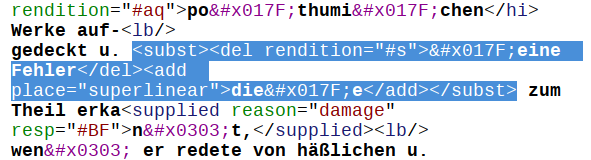
\includegraphics{Bilder/TEI2Graph/subst-xml-Beispiel.png}
\caption{XML-Beispiel aus der TEI-XML-Datei der Patzig-Vorlesungsmitschrift.}
\end{figure}

\begin{figure}
\centering
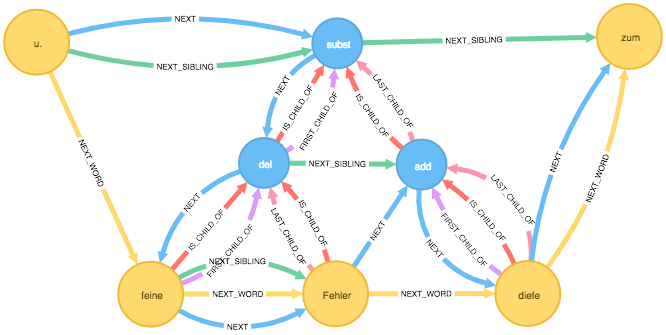
\includegraphics{Bilder/TEI2Graph/xml-importer-datenmodell.png}
\caption{XML-Beispiel im Graphen.}
\end{figure}

Beim Import der XML-Datei in den Graphen die XML-Element-Knoten in Xml-Tag-Knoten In der Abbildung des XML-Ausschnittes sind jene Teile blau markiert, die sich auch in der Graphabbildung befinden. Aus Sicht der XML-Hierarchie befindet sich der XML-Textknoten mit dem Inhalt \emph{gedeckt u.} auf der gleichen Ebene mit dem \texttt{\textless{}subst\textgreater{}}-Element. Dies wird beim

Mit dieser Modellierung lassen sich beispielsweise die von einem \texttt{\textless{}add\textgreater{}}-Element umfassten Wörter abfragen, in dem man ausgehend vom \texttt{add}-Knoten der \texttt{FIRT\_CHILD\_OF}-Kante rückwärts folgt, anschließend von diesem Knoten den \texttt{NEXT\_SIBLING}-Kanten so lange folgt, bis wieder die \texttt{LAST\_CHILD\_OF}-Kante wieder zum \texttt{add}-Knoten zurückführt. Der entsprechende cypher-Query sieht wie folgt aus:

\begin{verbatim}
MATCH
(n:XmlTag {_name:'add'})
<-[:FIRST_CHILD_OF]-(w1:XmlWord)
-[:NEXT_WORD*..5]->(w2:XmlWord)
-[:LAST_CHILD_OF]->(n)
RETURN * LIMIT 25
\end{verbatim}

\begin{figure}
\centering
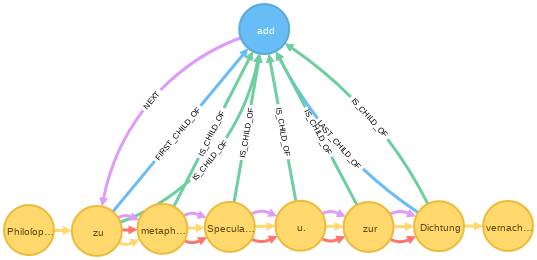
\includegraphics{Bilder/TEI2Graph/XML-Hierarchie.png}
\caption{XML-Hierarchie eines \texttt{\textless{}add\textgreater{}}-Elements und der von ihm umfassten Wörter im Graphen.}
\end{figure}

In einem zweiten Schritt kann der so entstandene Graph mit Hilfe von cypher-Querys weiter bearbeitet werden. Die Grahdatenbank neo4j ist schemafrei und somit können nun über die importieren XML-Strukturen weitere Erschließungsstrukturen gelegt werden, ohne dass ein XML-Parser sich über das nicht mehr wohlgeformte XML beschwert. Zu beachten ist bei jedem Schritt, ob wieder der Schritt zurück nach XML getätigt werden soll. Sicherlich ist es kein größeres Problem, eine in eine Graphdatenbank importierte XML-Datei wieder als solche zu exportieren. Ist der Graph aber mit weiteren Informationen angereichert, so muss geklärt werden, ob, und wenn ja wie, diese zusätzlichen Informationen in wohlgeformtes XML transferiert werden können.

\section{Das DTA-Basisformat im Graphen}\label{das-dta-basisformat-im-graphen}

Das DTA-Basisformat ist ein Subset der TEI und bietet für Textphänomene jeweils nur eine Möglichkeit der Auszeichnung. Damit wird die in der TEI vorhandene Flexibilität bei der Auszeichnung eingeschränkt, um damit einen höheren Grad an Interoperabilität zu erreichen. Das DTA-Basisformat folgt den P5-Richtlinien der TEI, trifft aber eine Tag-Auswahl der für die Auszeichung historischer Texte notwendigen Elemente.

Im folgenden Abschnitt werden für ausgewählte Elemente des DTA-Basisformats mögliche Modellierungsformen im Graphen beschrieben. Zum äußeren Erscheinungsbild wird der Seitenfall sowie Spalten- und Zeilenumbrüche berücksichtigt. Bei den Textphänomenen werden Absätze, Schwer- und Unleserliches und inhaltlich werden die Kapiteleinteilung, inhaltliche Inline-Auszeichnungen und editorische Eingriffe behandelt. Für die Metadaten werden keine Modellierungsvorschläge formuliert, da diese sich sauber im XML-Baum darstellen lassen und keine Überlappungsprobleme etc. entstehen.

\section{Strukturen des Dokuments}\label{strukturen-des-dokuments}

\subsection{Graphenmodellierung von Zeilen}\label{graphenmodellierung-von-zeilen}

Nehmen wir als Beispiel Zeilenwechsel auf einer Seite des Patzig-Manuskripts (http://www.deutschestextarchiv.de/book/view/patzig\_msgermfol841842\_1828/?hl=Himalaja\&p=39).\footnote{URL des Beispieltextes: http://www.deutschestextarchiv.de/book/view/patzig\_msgermfol841842\_1828/?hl=Himalaja\&p=39 abgerufen am 02.01.2018.}

\begin{Shaded}
\begin{Highlighting}[]
\NormalTok{... Die}\KeywordTok{<lb/>}
\NormalTok{Jnder hegen die große Verehrung vor}\KeywordTok{<lb/>}
\NormalTok{dem Himalaja Gebirge. ...}
\end{Highlighting}
\end{Shaded}

Im Graphen sieht die Stelle wie folgt aus:

\begin{figure}
\centering
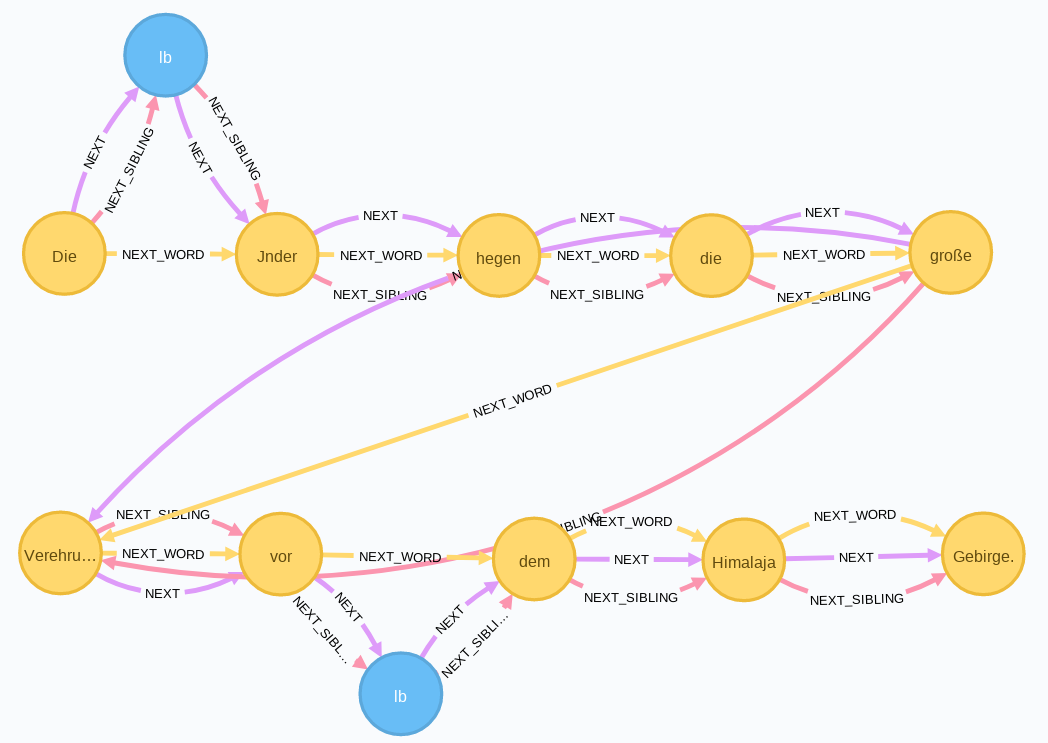
\includegraphics{Bilder/TEI2Graph/lb-im-Graph2.png}
\caption{\texttt{\textless{}lb/\textgreater{}}-Element im Graphen}
\end{figure}

Das leere \texttt{\textless{}lb/\textgreater{}}-Element steht für die Markierung eines Zeilenanfangs (\emph{line begins}). Der Graph soll nun so umgebaut werden, dass die Zeile durch einen \texttt{line}-Knoten gekennzeichnet wird, von dem aus eine \texttt{FIRST\_CHILD\_OF}-Kante mit dem ersten Wort der Zeile und eine \texttt{LAST\_CHILD\_OF}-Kante mit dem letzten Wort der Zeile verbunden ist.

Mit dem folgenden cypher-query kommt man den auf der Abbildung sichtbaren Subgraphen:

\begin{verbatim}
MATCH (n0:XmlWord)-[:NEXT_WORD]->
(n1:XmlWord {DtaID:10272})-[:NEXT_WORD*..8]->(n2:XmlWord),
(n1)<-[:NEXT]-(t1:XmlTag {_name:'lb'}),
(n3:XmlWord {DtaID:10277})-[:NEXT]->(t2:XmlTag {_name:'lb'})
RETURN * LIMIT 20;
\end{verbatim}

Im folgenden Schritt wird ein \texttt{line}-Knoten erzeugt, der die Zeile darstellen soll. Mit diesem werden dann das erste und das letzte Wort der Zeile verbunden.

\begin{verbatim}
MATCH (n0:XmlWord)-[:NEXT_WORD]->
(n1:XmlWord {DtaID:10272})-[:NEXT_WORD*..8]->(n2:XmlWord),
(n1)<-[:NEXT]-(t1:XmlTag {_name:'lb'}),
(n3:XmlWord {DtaID:10277})-[:NEXT]->(t2:XmlTag {_name:'lb'})
MERGE (n3)<-[:LAST_CHILD_OF]-(l:line {name:'line'})-[:FIRST_CHILD_OF]->(n1)
DETACH DELETE t1, t2
RETURN * LIMIT 20;
\end{verbatim}

Im Graphen sieht die Stelle wie folgt aus:

\begin{figure}
\centering
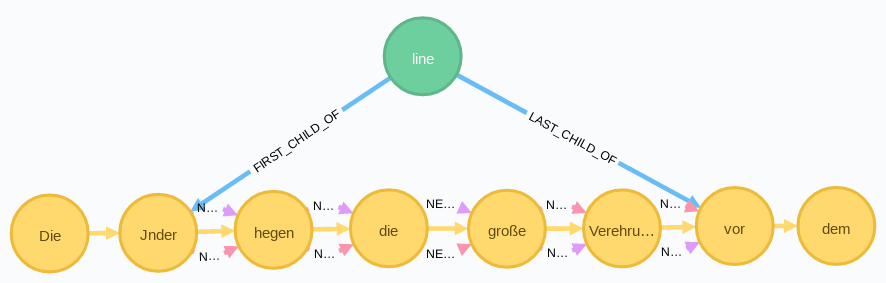
\includegraphics{Bilder/TEI2Graph/lb-to-line.png}
\caption{\texttt{\textless{}lb/\textgreater{}}-Element im Graphen}
\end{figure}

\subsection{Zeilenwechsel mit Worttrennungen}\label{zeilenwechsel-mit-worttrennungen}

Nun kommt es im Bereich der Zeilenwechsel sehr häufig zu Worttrennungen. Als Beispiel nehmen wir folgende Zeile, die sich auf der gleichen Seite wo das eben behandelte Beispiel befindet:

\begin{Shaded}
\begin{Highlighting}[]
\NormalTok{... Die Ken}\DecValTok{&#x0303;}\NormalTok{t-}\KeywordTok{<lb/>}
\NormalTok{niß des Jahres durch nicht von einer Nation}\KeywordTok{<lb/>}
\NormalTok{auf ...}
\end{Highlighting}
\end{Shaded}

Im Graphen sieht die Stelle wie folgt aus:

\begin{figure}
\centering
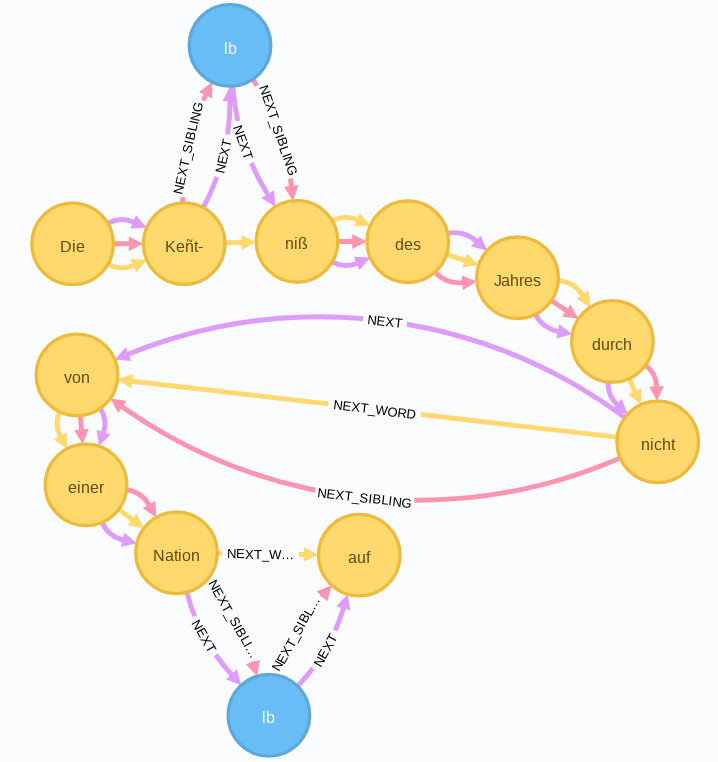
\includegraphics{Bilder/TEI2Graph/lb mit Worttrennung im Graphen.png}
\caption{\texttt{\textless{}lb/\textgreater{}}-Element im Graphen}
\end{figure}

Mit dem folgenden cypher-query kommt man den auf der Abbildung sichtbaren Supgraphen:

\begin{verbatim}
MATCH (n0:XmlWord {DtaID:10197})-[:NEXT_WORD]->
(n1:XmlWord)-[:NEXT_WORD*..9]->(n2:XmlWord),
(n1)-[:NEXT]->(t1:XmlTag {_name:'lb'}),
(n3:XmlWord {DtaID:10207})-[:NEXT]->(t2:XmlTag {_name:'lb'})
RETURN * LIMIT 20;
\end{verbatim}

Das \texttt{\textless{}lb/\textgreater{}}-Element trennt das Wort Kenntniß\footnote{Zur einfacheren Lesbarkeit wurden im Wort \emph{Kenntniß} die Sonderzeichen normalisiert.}. Im nächsten Schritt werden nun die beiden getrennten Wortknoten \texttt{Kennt-} und \texttt{niß} im zweiten Wortknoten \texttt{niß} zusammengefasst. Der erste Wortknoten \texttt{Kennt-} inkl. seiner Kanten wird gelöscht und eine neue NEXT-Kante zwischen dem \texttt{niß}-Wortknoten und dem vorhergehenden \texttt{Die}-Wortknoten erstellt. Die Informationen, an welcher Stelle das Wort getrennt war, wird in den Eigenschaften des neuen \texttt{Kenntniß}-Wortnnotens gespeichert. In der Eigenschaft \texttt{before} steht dann der Inhalt des ursprünlich ersten Wortknotens \texttt{Kennt-} und in der Eigenschaft after der Inhalt des ursprünglich zweiten Wortknotens \texttt{niß}.

Hier werden die notwendigen Cypher-Befehle angezeigt:

\begin{verbatim}
MATCH (n0:XmlWord {DtaID:10197})-[:NEXT_WORD]->
(n1:XmlWord {DtaID:10198})-[:NEXT_WORD]->
(n2:XmlWord {DtaID:10200})-[:NEXT_WORD*..8]->(n3:XmlWord {DtaID:10207}),
(n1)-[:NEXT]->(t1:XmlTag {_name:'lb'}),
(n4:XmlWord {DtaID:10207})-[:NEXT]->(t2:XmlTag {_name:'lb'})
SET n2.before = left(n1.text, size(n1.text)-1)
SET n2.after = n2.text
SET n2.text = left(n1.text, size(n1.text)-1)+n2.after
MERGE (n0)-[:NEXT_WORD]->(n2)
MERGE (n4)<-[:LAST_CHILD_OF]-(l:line {name:'line'})-[:FIRST_CHILD_OF]->(n2)
DETACH DELETE t1, t2, n1
RETURN * LIMIT 20;
\end{verbatim}

Im Graphen ergibt sich anschließend folgendes Bild:

\begin{figure}
\centering
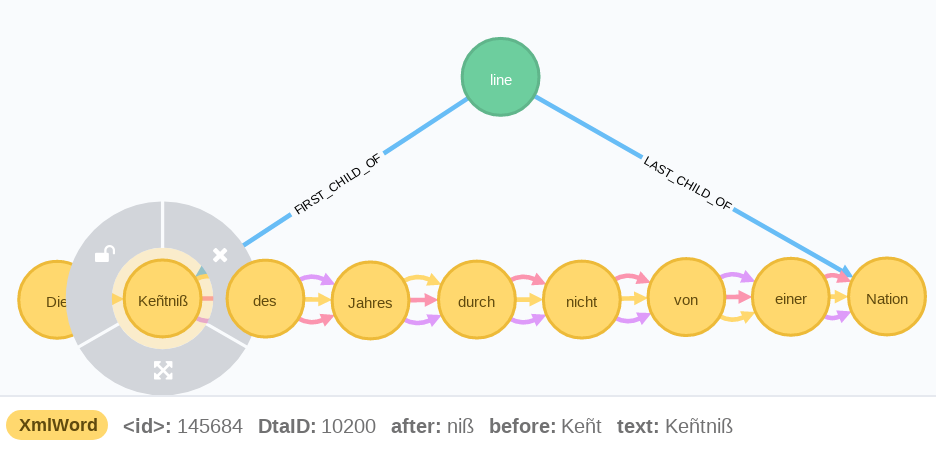
\includegraphics{Bilder/TEI2Graph/lb-Trennung-rausgenommen2.png}
\caption{\texttt{\textless{}lb/\textgreater{}}-Element im Graphen herausgenommen, Wortknoten zusammengefasst}
\end{figure}

Am unteren Bereich der Abbildung sind in der Legende die Propertys des Wortknotens \emph{Kentniß} hervorgehoben. Dort erkennt man die vorher vorhandenen Wortbestandteile und den neuen Wert der Property \emph{text}.

\subsection{Seitenzahlen und Faksimilezählung}\label{seitenzahlen-und-faksimilezuxe4hlung}

Im DTA-Bf wird jeweils der Anfang einer Seite mit dem leeren Element \texttt{\textless{}pb\textgreater{}} markiert\footnote{Vgl. die Dokumentation des DTA-Basisformats unter http://www.deutschestextarchiv.de/doku/basisformat/seitenFacsNr.html abgerufen am 25.11.2017.}. Das leere Element kann noch die Attribute \texttt{facs} für die Zählung der Faksimileseiten und \texttt{n} für die auf der Seite ggf. angegebene Seitenzahl enthalten.

\begin{Shaded}
\begin{Highlighting}[]
\KeywordTok{<pb}\OtherTok{ facs=}\StringTok{"#f[Bildnummer]"}\OtherTok{ n=}\StringTok{"[Seitenzahl]"}\KeywordTok{/>}
\end{Highlighting}
\end{Shaded}

Ist eine Seitenzahl im Faksimile falsch wiedergegeben, so wird diese originalgetreu übernommen und die richtige Seitenzahl in eckigen hinzugefügt in das \texttt{n}-Attribut übernommen.

\begin{Shaded}
\begin{Highlighting}[]
\KeywordTok{<pb}\OtherTok{ facs=}\StringTok{"#f[Bildnummer]"}\OtherTok{ n=}\StringTok{"[fehlerhafte Seitenzahl [korrigierte Seitenzahl]]"}\KeywordTok{/>}
\end{Highlighting}
\end{Shaded}

Das \texttt{\textless{}pb/\textgreater{}}-Element auf den Seiten 5 und 6 aus Patzig (http://www.deutschestextarchiv.de/book/view/patzig\_msgermfol841842\_1828/?hl=viel\&p=5)\footnote{Die Beispielseite findet sich unter http://www.deutschestextarchiv.de/book/view/patzig\_msgermfol841842\_1828/?p=5 abgerufen am 25.11.2017.}:

\begin{Shaded}
\begin{Highlighting}[]
\NormalTok{... Abwe}\DecValTok{&#x017F;}\NormalTok{enheit vom heimi}\DecValTok{&#x017F;}\NormalTok{chen Boden ent-}\KeywordTok{<lb/>}
\KeywordTok{<note}\OtherTok{ place=}\StringTok{"left"}\KeywordTok{><figure}\OtherTok{ type=}\StringTok{"stamp"}\KeywordTok{/><lb/>}
\KeywordTok{</note>}\NormalTok{fernt hielt, der }\DecValTok{&#x017F;}\NormalTok{ich viel mit einem Volke}\KeywordTok{<lb/>}
\KeywordTok{<fw}\OtherTok{ place=}\StringTok{"bottom"}\OtherTok{ type=}\StringTok{"catch"}\KeywordTok{>}\NormalTok{befreun-}\KeywordTok{</fw><lb/>}
\KeywordTok{<pb}\OtherTok{ facs=}\StringTok{"#f0006"}\OtherTok{ n=}\StringTok{"2."}\KeywordTok{/>}
\NormalTok{befreundete, welches durch den}
\NormalTok{...}
\NormalTok{in einzelnen großen Zügen zu ent-}\KeywordTok{<lb/>}
\NormalTok{werfen}\ErrorTok{<}\NormalTok{/hi>.}\ErrorTok{<}\NormalTok{/p>}\KeywordTok{<lb/>}
\KeywordTok{<fw}\OtherTok{ place=}\StringTok{"bottom"}\OtherTok{ type=}\StringTok{"catch"}\KeywordTok{>}\NormalTok{Nachdem}\KeywordTok{</fw><lb/>}
\KeywordTok{<pb}\OtherTok{ facs=}\StringTok{"#f0007"}\OtherTok{ n=}\StringTok{"3."}\KeywordTok{/>}
\KeywordTok{<p><note}\OtherTok{ place=}\StringTok{"left"}\KeywordTok{><hi}\OtherTok{ rendition=}\StringTok{"#u"}\KeywordTok{>}\NormalTok{Neue}\DecValTok{&#x017F;}\NormalTok{te A}\DecValTok{&#x017F;}\NormalTok{tronomi}\DecValTok{&#x017F;}\NormalTok{che Ent-}\KeywordTok{<lb/>}
\NormalTok{deckungen.}\KeywordTok{</hi><lb/>}\NormalTok{ ...}
\end{Highlighting}
\end{Shaded}

Im Graphen findet man das \texttt{\textless{}pb\textgreater{}}-Element der Seite 6 mit folgendem Query{[}\^{}a825{]}:

\begin{verbatim}
MATCH
(n1:XmlWord {DtaID:869})-[:NEXT]->
(lb1:XmlTag {_name:'lb'})-[:NEXT]->
(t2:XmlTag {_name:'fw', place:'bottom', type:'catch'})-[:NEXT_SIBLING]->
(lb2:XmlTag {_name:'lb'})-[:NEXT_SIBLING]->
(pb:XmlTag {_name:'pb'}),
(n1:XmlWord)-[nw1:NEXT_WORD]->
(n2:XmlWord)-[nw2:NEXT_WORD]->
(n3:XmlWord)-[nw3:NEXT_WORD]->
(n4:XmlWord),
(n2:XmlWord)-[:NEXT]->(t1:XmlTag {_name:'lb'})
RETURN * LIMIT 20;
\end{verbatim}

Im Graphen ergibt sich folgendes Bild:

\begin{figure}
\centering
\includegraphics{Bilder/TEI2Graph/pb6-Bestand.png}
\caption{Der Pfad vom \texttt{\textless{}pb/\textgreater{}}-Element zum ersten Wort der Seite \emph{befreundet}.}
\end{figure}

Markiert ist das \texttt{\textless{}pb/\textgreater{}}-Element der Seite 6. Im Fuß der Abbildung werden die Propertys des Elements angezeigt. Der Textfluss wird durch den Wortknoten \texttt{befreun-} unterbrochen, der eine Kustode darstellt. Diese soll aus dem Textfluss herausgelöst und direkt mit dem letzten Wortknoten \texttt{Volke} über die neu eingeführte \texttt{catch\_words}-Kante verbunden werden. Der \texttt{\textless{}fw\textgreater{}}, und der \texttt{\textless{}lb/\textgreater{}}-Knoten werden gelöscht und der letzte Wortknoten der Seite über eine neue \texttt{NEXT}-Kante mit dem \texttt{\textless{}pb/\textgreater{}}-Knoten verknüpft.

Hier der Query für den Umbau:

\begin{verbatim}
MATCH
(n1:XmlWord {DtaID:869})-[:NEXT]->
(lb1:XmlTag {_name:'lb'})-[:NEXT]->
(t2:XmlTag {_name:'fw', place:'bottom', type:'catch'})-[:NEXT_SIBLING]->
(lb2:XmlTag {_name:'lb'})-[:NEXT_SIBLING]->
(pb:XmlTag {_name:'pb'}),
(n1:XmlWord)-[nw1:NEXT_WORD]->
(n2:XmlWord)-[nw2:NEXT_WORD]->
(n3:XmlWord)-[nw3:NEXT_WORD]->
(n4:XmlWord),
(n2:XmlWord)-[:NEXT]->(t1:XmlTag {_name:'lb'})
DELETE nw1, nw2
DETACH DELETE t2
MERGE (n1)-[:NEXT_WORD]->(n3)
MERGE (n1)-[:CATCH_WORDS]->(n2)
MERGE (n1)-[:NEXT_WORD]->(n3)
MERGE (lb1)-[:NEXT]->(n2)
RETURN * LIMIT 20;
\end{verbatim}

Im Graphen ergibt sich folgendes Bild:

\begin{figure}
\centering
\includegraphics{Bilder/TEI2Graph/fw-catch-words.png}
\caption{Die Kustode \emph{befreun-} wird aus der \texttt{NEXT\_WORD}-Textkette herausgenommen und über eine \texttt{CATCH\_WORDS}-Kante mit dem Wortknoten \emph{Volke} verknüpft.}
\end{figure}

Die Kustode ist nun nicht mehr über \texttt{NEXT\_WORD}-Kanten mit dem Fließtext verknüpft, bleibt aber über die \texttt{CATCH\_WORDS}-Kante mit dem letzten Wort der Seite verbunden. In einem zweiten Schritt müssen nun die beiden \texttt{\textless{}pb/\textgreater{}}-Elementknoten zu einem neu einzuführenden \texttt{page}-Knoten zusammengeführt werden. Hierfür lassen wir uns im nächsten cypher-Query alle \texttt{\textless{}pb/\textgreater{}}-Knoten mit einer DtaID kleiner als 875 anzeigen, da diese vor dem \texttt{\textless{}pb/\textgreater{}}-Knoten der Seite 6 mit der DtaID 874 liegen:

\begin{verbatim}
MATCH (n:XmlTag {_name:'pb'})
WHERE n.DtaID < 875
RETURN n;
\end{verbatim}

\begin{figure}
\centering
\includegraphics{Bilder/TEI2Graph/pb-Element-Tabelle.png}
\caption{Tabellenansicht aller \texttt{\textless{}pb/\textgreater{}}-Knoten mit einer DtaID kleiner als 875.}
\end{figure}

Aus der Tabellenansicht ist zu entnehmen, dass Seite 5 von den \texttt{\textless{}pb/\textgreater{}}-Elementen mit der DtaID 562 und 874 eingefasst wird.

Der cypher-Query zum Einfügen des \texttt{page}-Knoten sieht wie folgt aus:

\begin{verbatim}
MATCH
(pb1:XmlTag {DtaID:562, _name:'pb'})-[n1:NEXT*..5]->(w1:XmlWord {DtaID:565}),
(pb2:XmlTag {DtaID:874, _name:'pb'})<-[n2:NEXT*..5]-(w2:XmlWord {DtaID:872})
MERGE
(w1)<-[:FIRST_CHILD_OF]-(page:page {facs:'#f0005', n:1})-[:LAST_CHILD_OF]->(w2)
RETURN pb1, w1, pb2, w2, page;
\end{verbatim}

\begin{figure}
\centering
\includegraphics{Bilder/TEI2Graph/page-f0005.png}
\caption[Die Seite wird modelliert mit dem \texttt{page}-Knoten \#0005 der mit dem ersten Wort über eine \texttt{FIRST\_CHILD\_OF}- und mit dem letzten Wort der Seite über eine \texttt{LAST\_CHILD\_OF}-Kante verknüpft ist.]{Die Seite wird modelliert mit dem \texttt{page}-Knoten \#0005 der mit dem ersten Wort über eine \texttt{FIRST\_CHILD\_OF}- und mit dem letzten Wort der Seite über eine \texttt{LAST\_CHILD\_OF}-Kante verknüpft ist.\footnotemark{}}
\end{figure}
\footnotetext{Die Darstellung der Wortkette ist zwischen den Wortknoten \emph{der} und \emph{einem} zu Gunsten der Übersichtlichkeit gekürzt.}

\subsection{Absätze}\label{absuxe4tze}

Absätze werden im DTA-Basisformat mit dem \texttt{\textless{}p\textgreater{}}-Element eingefasst. Im Manusskript von Patzig finden sich insgesamt 238 mit dem \texttt{\textless{}p\textgreater{}}-Element eingefasste Textabschnitte\footnote{Die Anzahl der \texttt{\textless{}p\textgreater{}}-Elemente im Graph erhält man mit der Abfrage MATCH (n:XmlTag \{\_name:`p'\}) RETURN count(n);}.

\begin{figure}
\centering
\includegraphics{Bilder/TEI2Graph/p-xml-Beispiel.png}
\caption{XML-Auszug aus Patzig mit einem Absatz als Beispiel.}
\end{figure}

Da das \texttt{\textless{}p\textgreater{}}-Element im Unterschied zu den leeren Elementen wie \texttt{pb} oder \texttt{lb} ein öffnendes und schließendes Tag hat, wird beim Import der TEI-Xml-Datei durch den Importer schon ein \texttt{p}-Knoten erstellt, der mit einer \texttt{FIRST\_CHILD\_OF}-Kante mit dem ersten Wort des Absatzes und mit einer \texttt{LAST\_CHILD\_OF}-Kante mit dem letzten Wort des Absatzes verknüpft ist.

\begin{figure}
\centering
\includegraphics{Bilder/TEI2Graph/p-graph-Beispiel.png}
\caption{Ein Teil des gleichen Absatzes aus Patzig im Graphen.}
\end{figure}

Alle Wörter eines Absatzes sind darüber hinaus über \texttt{NEXT\_SIBLING}-Kanten in der Textreihenfolge verknüpft.

\subsection{Kapiteleinteilung}\label{kapiteleinteilung}

Im DTA-Basisformat wird bei der Transkiption von Büchern die Kapiteleinteilung mit verschachtelten \texttt{div}-Element vorgenommen. Das im \texttt{div}-Element erlaubte @n-Attribut gibt die Strukturebene an. Über das @type-Attribut kann der Typ des Kapitels näher spezifiziert werden. Eine Liste der möglichen Werte für das Attribut findet sich unter http://deutschestextarchiv.de/doku/basisformat/div.html.

Für Manuskripte, wie der hier behandelten Vorlesungsmitschrift von Patzig gibt es unter http://deutschestextarchiv.de/doku/basisformat/msKapitel.html noch zwei zusätzliche Werte für das @type-Attribut, nämlich \emph{session} für Vorlesungsmitschriften und \emph{letter} für Briefe.

Mit folgendem cypher-Query erhalten wir die in Patzig verwendeten Werte für das @type-Attribut des \texttt{div}-Elements.

\begin{verbatim}
MATCH (n:XmlTag {_name:'div'})
RETURN n.type, count(n.type) AS Anzahl ORDER BY Anzahl DESC;
\end{verbatim}

\begin{longtable}[]{@{}lr@{}}
\toprule
n.type & Anzahl\tabularnewline
\midrule
\endhead
session & 62\tabularnewline
null & 0\tabularnewline
\bottomrule
\end{longtable}

Es sind also insgesamt 62 Kapitel vom Typ \emph{session} (Vorlesungsmitschrift) enthalten. Mit folgendem cypher-Query wird die Kapitelstruktur der ersten Kapitel und der darunter liegenden Ebenen bis zum jeweils ersten und letzten Wort des Kapitels angezeigt.

\begin{verbatim}
MATCH
p1 = shortestPath(
    (div:XmlTag {_name:'div'})<-[:FIRST_CHILD_OF*..20]-(w1:XmlWord)),
p2 = shortestPath(
    (div:XmlTag {_name:'div'})<-[:LAST_CHILD_OF*..20]-(w2:XmlWord))
RETURN p1,p2 LIMIT 20;
\end{verbatim}

\begin{figure}
\centering
\includegraphics{Bilder/TEI2Graph/div-Struktur-XmlWord.png}
\caption{Struktur der ersten Kapitel mit dem jeweils ersten und letzten Wort.}
\end{figure}

Mit dem folgenden cypher-Query wird das erste Wort des Kapitels über eine \texttt{FIRST\_CHILD\_OF}-Kante und das letzte Wort des Absatzes über eine \texttt{LAST\_CHILD\_OF}-Kante mit dem \texttt{div}-Knoten verbunden. Um die neu erstellen Kanten von den vom Importer erstellen zu unterscheiden erhalten diese die Proptery \emph{type} mit dem Wert \emph{graph}. Um die \texttt{div}-Knoten von den anderen \texttt{XmlTag}-Knoten unterscheiden zu können erhalten sie das zusätzliche Label \emph{Session}.

\begin{verbatim}
MATCH
p1 = shortestPath(
    (div:XmlTag {_name:'div'})<-[:FIRST_CHILD_OF*..20]-(w1:XmlWord)
    ),
p2 = shortestPath(
    (div:XmlTag {_name:'div'})<-[:LAST_CHILD_OF*..20]-(w2:XmlWord)
    )
MERGE (w1)-[:FIRST_CHILD_OF {type:'graph'}]->
    (div)<-[:LAST_CHILD_OF {type:'graph'}]-(w2)
SET div:Session
RETURN * LIMIT 20;
\end{verbatim}

\subsection{Zusammenfassung}\label{zusammenfassung-4}

In diesem Kapitel wurden exemplarisch die XML-Strukturen für Zeilen (\texttt{lb}), Seiten (\texttt{pb}), Absätze (\texttt{p}) und Kapitel (\texttt{div}) in Graphstrukturen überführt, in denen jedes Element nur noch aus einem Knoten besteht. Mit diesem Knoten wird jeweils das erste und das letzte betroffene Wort mit einer \texttt{FIRST\_CHILD\_OF}- und einer \texttt{LAST\_CHILD\_OF}-Kante verknüpft. Damit entstehen offensichtlich überlappende Strukturen, was im Graphen aber kein Problem darstellt.

\section{Editorische Eingriffe}\label{editorische-eingriffe}

\subsection{Hinzufügungen und Tilgungen}\label{hinzufuxfcgungen-und-tilgungen}

Die Elemente \texttt{\textless{}add\textgreater{}} und \texttt{\textless{}del\textgreater{}} werden für Kennzeichnung von Tilgungen und Hinzufügungen des Autors oder von späteren Bearbeitern verwendet.

\subsubsection{\texorpdfstring{\texttt{\textless{}add\textgreater{}}-Element}{\textless{}add\textgreater{}-Element}}\label{add-element}

Dabei können die Umstände der Änderungen beim \texttt{\textless{}add\textgreater{}}-Element mit dem @place-Attribut näher beschrieben, welches die in der folgenden Tabelle angegebenen Werte annehmen darf\footnote{Vgl. hierzu http://deutschestextarchiv.de/doku/basisformat/msAddDel.html.}:

\begin{longtable}[]{@{}lll@{}}
\toprule
Element & @place-Wert & Bedeutung\tabularnewline
\midrule
\endhead
\texttt{\textless{}add\textgreater{}} & superlinear & über der Zeile eingetragen\tabularnewline
\texttt{\textless{}add\textgreater{}} & sublinear & unter der Zeile eingetragen\tabularnewline
\texttt{\textless{}add\textgreater{}} & intralinear & innerhalb der Zeile eingetragen\tabularnewline
\texttt{\textless{}add\textgreater{}} & across & über den ursprünglichen Text geschrieben\tabularnewline
\texttt{\textless{}add\textgreater{}} & left & am linken Rand eingetragen\tabularnewline
\texttt{\textless{}add\textgreater{}} & right & am rechten Rand eingetragen\tabularnewline
\bottomrule
\end{longtable}

Mit folgenden cypher-Query erhält man die Verteilung der Attributwerte.

\begin{verbatim}
MATCH (n:XmlTag {_name:'add'})
RETURN n.place, count(n.place) AS Anzahl ORDER BY Anzahl DESC;
\end{verbatim}

\begin{longtable}[]{@{}lr@{}}
\toprule
n.place & Anzahl\tabularnewline
\midrule
\endhead
across & 436\tabularnewline
superlinear & 268\tabularnewline
intralinear & 60\tabularnewline
left & 16\tabularnewline
sublinear & 2\tabularnewline
\bottomrule
\end{longtable}

\subsubsection{\texorpdfstring{\texttt{\textless{}del\textgreater{}}-Element}{\textless{}del\textgreater{}-Element}}\label{del-element}

Die mit dem \texttt{\textless{}del\textgreater{}}-Element gekennzeichneten Tilgungen können mit dem @rendition-Attribut näher beschrieben werden, dessen mögliche Werte in der folgenden Tabelle angegeben sind\footnote{Vgl. hierzu http://deutschestextarchiv.de/doku/basisformat/msAddDel.html.}.

\begin{longtable}[]{@{}lll@{}}
\toprule
Element & @rendition-Wert & Bedeutung\tabularnewline
\midrule
\endhead
\texttt{\textless{}del\textgreater{}} & \#ow & Tilgung durch Überschreibung des ursprünglichen Textes\tabularnewline
\texttt{\textless{}del\textgreater{}} & \#s & Tilgung durch Streichung\tabularnewline
\texttt{\textless{}del\textgreater{}} & \#erased & Tilgung durch Radieren, Auskratzen\tabularnewline
\bottomrule
\end{longtable}

Mit folgenden cypher-Query erhält man die Verteilung der Attributwerte.

\begin{verbatim}
MATCH (n:XmlTag {_name:'add'})
RETURN n.rendition, count(n.rendition) AS Anzahl
ORDER BY Anzahl DESC;
\end{verbatim}

\begin{longtable}[]{@{}lr@{}}
\toprule
n.rendition & Anzahl\tabularnewline
\midrule
\endhead
\#ow & 436\tabularnewline
\#s & 268\tabularnewline
\#erased & 60\tabularnewline
\bottomrule
\end{longtable}

\subsubsection{\texorpdfstring{Umbau von \texttt{\textless{}add\textgreater{}}- und \texttt{\textless{}del\textgreater{}}-Elementen in einer \texttt{\textless{}subst\textgreater{}}-Umgebung}{Umbau von \textless{}add\textgreater{}- und \textless{}del\textgreater{}-Elementen in einer \textless{}subst\textgreater{}-Umgebung}}\label{umbau-von-add--und-del-elementen-in-einer-subst-umgebung}

Der Umbau wird an einem Beispieltext der Seite 32 des Patzig-Manuskripts durchgeführt\footnote{Vgl. http://www.deutschestextarchiv.de/book/view/patzig\_msgermfol841842\_1828/?hl=zum\&p=32.}.

\begin{figure}
\centering
\includegraphics{Bilder/TEI2Graph/subst-xml-Beispiel.png}
\caption{-Beispiel in der XML-Ansicht.}
\end{figure}

Im Graphen findet man die entsprechende Stelle mit folgendem cypher-Query.

\begin{verbatim}
MATCH
(w1:XmlWord)-[r1:NEXT_WORD]->
(w2:XmlWord)-[r2:FIRST_CHILD_OF]->
(t1)-[r3:FIRST_CHILD_OF]->
(s:XmlTag {_name:'subst', DtaID:8248})
<-[r4:LAST_CHILD_OF]-(t2)
<-[r5:LAST_CHILD_OF]-(w4:XmlWord)
-[r6:NEXT_WORD]->(w5:XmlWord),
(w2)-[r7:NEXT_WORD]->(w3)-[r8:NEXT_WORD]->(w4)
RETURN *;
\end{verbatim}

Der Query gruppiert sich um den \texttt{s}-Knoten, der das \texttt{subst}-Element darstellt und es über die DtaID identifiziert. Vom \texttt{s}-Knoten ausgehend, folgt der Pfad einerseits über \texttt{FIRST\_CHILD\_OF}-Kanten zum \texttt{n3}-Knoten (add-Element) und zum \texttt{n2}-Knoten, der schließlich das Wort \emph{seine} darstellt. Über die \texttt{LAST\_CHILD\_OF}-Kante geht es zum \texttt{n4}-Knoten (del-Element) zum \texttt{n5}-Wortknoten, der das Wort \emph{diese} darstellt. Im zweiten Teil des MATCH-Befehls wird der Pfad zwischen dem Wort \emph{seine} und \emph{diese} ermittelt und schließlich alles ausgegeben.

\begin{figure}
\centering
\includegraphics{Bilder/TEI2Graph/subst-graph-1.png}
\caption{-Beispiel in der Graph-Ansicht.}
\end{figure}

cyper-Query für den umgebaut

\begin{verbatim}
MATCH
(w1:XmlWord)-[r1:NEXT_WORD]->
(w2:XmlWord)-[r2:FIRST_CHILD_OF]->
(t1)-[r3:FIRST_CHILD_OF]->
(s:XmlTag {_name:'subst', DtaID:8248})
<-[r4:LAST_CHILD_OF]-(t2)
<-[r5:LAST_CHILD_OF]-(w4:XmlWord)
-[r6:NEXT_WORD]->(w5:XmlWord),
(w2)-[r7:NEXT_WORD]->(w3)-[r8:NEXT_WORD]->(w4)
DELETE r1, r8
SET r8.variant_type='add'
CREATE (w1)-[:NEXT_WORD{variant_type:'add'}]->(w4)
CREATE (w1)-[:NEXT_WORD{variant_type:'del'}]->(w2)
CREATE (w3)-[:NEXT_WORD{variant_type:'del'}]->(w5)
SET r7.variant_type='del'
RETURN *;
\end{verbatim}

Das Ergebnis erhält man über den folgenden Query.

\begin{verbatim}
MATCH
(w1:XmlWord)-[r1:NEXT_WORD]->
(w2:XmlWord)-[r2:FIRST_CHILD_OF]->
(t1)-[r3:FIRST_CHILD_OF]->
(s:XmlTag {_name:'subst', DtaID:8248})
<-[r4:LAST_CHILD_OF]-(t2)
<-[r5:LAST_CHILD_OF]-(w4:XmlWord)
-[r6:NEXT_WORD]->(w5:XmlWord),
(w2)-[r7:NEXT_WORD]->(w3)-[r8:NEXT_WORD]->(w4)
\end{verbatim}

\begin{figure}
\centering
\includegraphics{Bilder/TEI2Graph/subst-add-del-bearbeitet.png}
\caption{\textless{}subst\textgreater{}-Beispiel nach dem Graph-Umbau.}
\end{figure}

\chapter{JSON Import mit den Daten der Germania Sacra}\label{json-import-mit-den-daten-der-germania-sacra}

(Dieser Abschnitt befindet sich in Bearbeitung)

\section{Das Projekt Germania Sacra}\label{das-projekt-germania-sacra}

Das Projekt Germania Sacra erschließt die Quellen der Kirche des alten Reiches.{[}\^{}eeaa{]} Dabei werden die Kirche und ihre Institutionen von den Anfängen im 3./4. Jahrhundert bis zu deren Auflösung am Beginn des 19. Jahrhunderts dar. Im Rahmen des Projekts werden die überlieferten Quellen nach einheitlichen Kriterien aufgearbeitet und so strukturierte Daten für Kirchengeschichte im alten Reich bereitgestellt. So bildet das Projekt die Grundlage für weiterführende Forschungen.

Neben den Bänden bietet das Projekt auch ein \href{https://adw-goe.de/forschung/forschungsprojekte-akademienprogramm/germania-sacra/digitales-personenregister/}{digitales Personenregister} mit Angaben u.a. zu Personen, Bischöfen, Klöstern und Stiften. Die Daten werden über die \href{https://adw-goe.de/forschung/forschungsprojekte-akademienprogramm/germania-sacra/schnittstellen-und-linked-data/}{Schnittstellen des Projekts} als JSON-Daten bereitgestellt.\footnote{Der in diesem Kapitel verwendete json-Dump wurde freundlicherweise direkt vom Projekt Germania Sacra zur Verfügung gestellt und die Verwendung in dieser Veröffentlichung sowie die weitere Verwendung genehmigt.}

\section{Germania Sacra JSON}\label{germania-sacra-json}

\subsection{Personen}\label{personen}

Die Daten des Projekts umfassen z.B. Angaben zu Namen, Namensalternativen, Daten zu den Personen und der institutionelle Anbindung. Der folgende Ausschnitt aus einer JSON-Datei umfasst beispielhaft zwei Personeneinträge.

\begin{Shaded}
\begin{Highlighting}[]
\FunctionTok{\{}
    \DataTypeTok{"persons"}\FunctionTok{:} \OtherTok{[}\FunctionTok{\{}
        \DataTypeTok{"person_vorname"}\FunctionTok{:} \StringTok{"Ludold"}\FunctionTok{,}
        \DataTypeTok{"person_name"}\FunctionTok{:} \StringTok{"Ludold von Escherde"}\FunctionTok{,}
        \DataTypeTok{"person_namensalternativen"}\FunctionTok{:} \StringTok{"von Goltern (?)"}\FunctionTok{,}
        \DataTypeTok{"person_gso"}\FunctionTok{:} \StringTok{"060-02673-001"}\FunctionTok{,}
        \DataTypeTok{"person_gnd"}\FunctionTok{:} \StringTok{""}\FunctionTok{,}
        \DataTypeTok{"person_bezeichnung"}\FunctionTok{:} \StringTok{"Abt"}\FunctionTok{,}
        \DataTypeTok{"person_bezeichnung_plural"}\FunctionTok{:} \StringTok{"}\CharTok{\textbackslash{}u00c4}\StringTok{bte"}\FunctionTok{,}
        \DataTypeTok{"person_anmerkung"}\FunctionTok{:} \StringTok{""}\FunctionTok{,}
        \DataTypeTok{"person_von_verbal"}\FunctionTok{:} \StringTok{"1234"}\FunctionTok{,}
        \DataTypeTok{"person_von"}\FunctionTok{:} \DecValTok{1234}\FunctionTok{,}
        \DataTypeTok{"person_bis_verbal"}\FunctionTok{:} \StringTok{"1263"}\FunctionTok{,}
        \DataTypeTok{"person_bis"}\FunctionTok{:} \DecValTok{1263}\FunctionTok{,}
        \DataTypeTok{"person_office_id"}\FunctionTok{:} \StringTok{"282620"}
    \FunctionTok{\}}\OtherTok{,} \FunctionTok{\{}
        \DataTypeTok{"person_vorname"}\FunctionTok{:} \StringTok{"Hermann"}\FunctionTok{,}
        \DataTypeTok{"person_name"}\FunctionTok{:} \StringTok{"Hermann"}\FunctionTok{,}
        \DataTypeTok{"person_namensalternativen"}\FunctionTok{:} \StringTok{""}\FunctionTok{,}
        \DataTypeTok{"person_gso"}\FunctionTok{:} \StringTok{"033-02024-001"}\FunctionTok{,}
        \DataTypeTok{"person_gnd"}\FunctionTok{:} \StringTok{""}\FunctionTok{,}
        \DataTypeTok{"person_bezeichnung"}\FunctionTok{:} \StringTok{"Abt"}\FunctionTok{,}
        \DataTypeTok{"person_bezeichnung_plural"}\FunctionTok{:} \StringTok{"}\CharTok{\textbackslash{}u00c4}\StringTok{bte"}\FunctionTok{,}
        \DataTypeTok{"person_anmerkung"}\FunctionTok{:} \StringTok{""}\FunctionTok{,}
        \DataTypeTok{"person_von_verbal"}\FunctionTok{:} \StringTok{"1262"}\FunctionTok{,}
        \DataTypeTok{"person_von"}\FunctionTok{:} \DecValTok{1262}\FunctionTok{,}
        \DataTypeTok{"person_bis_verbal"}\FunctionTok{:} \StringTok{"1265"}\FunctionTok{,}
        \DataTypeTok{"person_bis"}\FunctionTok{:} \DecValTok{1265}\FunctionTok{,}
        \DataTypeTok{"person_office_id"}\FunctionTok{:} \StringTok{"311579"}
    \FunctionTok{\}}
\end{Highlighting}
\end{Shaded}

Die folgende Abbildung zeigt beispielhaft den ersten Personeneintrag des obigen json-Beispiels von Ludold von Escherde als importierten Personenknoten im Graphen.

\begin{figure}
\centering
\includegraphics{Bilder/Germania-Sacra-Personenknoten-mit-Properties.png}
\caption{Personenknoten von Ludold von Escherde in der Graphdatenbank}
\end{figure}

Unter dem Personenknoten werden die aus dem json importierten Properties aufgelistet.

\subsection{Klöster}\label{kluxf6ster}

Die folgende Abbildung zeigt die ersten drei Einträge der JSON-Datei mit den Angaben zu den Klöstern.

\begin{Shaded}
\begin{Highlighting}[]
\FunctionTok{\{}\DataTypeTok{"kloster"}\FunctionTok{:}
\OtherTok{[}
 \FunctionTok{\{}
   \DataTypeTok{"bezeichnung"}\FunctionTok{:} \StringTok{"Adeliges Damenstift Neuburg"}\FunctionTok{,}
   \DataTypeTok{"ort"}\FunctionTok{:} \StringTok{"Heidelberg"}\FunctionTok{,}
   \DataTypeTok{"bistum"}\FunctionTok{:} \StringTok{"Worms"}\FunctionTok{,}
   \DataTypeTok{"klosterid"}\FunctionTok{:} \DecValTok{20595}\FunctionTok{,}
   \DataTypeTok{"Wikipedia"}\FunctionTok{:} \StringTok{"#http://de.wikipedia.org/wiki/Abtei_Neuburg#"}\FunctionTok{,}
   \DataTypeTok{"GND"}\FunctionTok{:} \StringTok{"#http://d-nb.info/gnd/4316849-8#"}\FunctionTok{,}
   \DataTypeTok{"GeonameID_Ortsname"}\FunctionTok{:} \DecValTok{2907911}\FunctionTok{,}
   \DataTypeTok{"Datum_von"}\FunctionTok{:} \DecValTok{1671}\FunctionTok{,}
   \DataTypeTok{"Datum_bis"}\FunctionTok{:} \DecValTok{1681}
 \FunctionTok{\}}\OtherTok{,}
 \FunctionTok{\{}
   \DataTypeTok{"bezeichnung"}\FunctionTok{:} \StringTok{"Adeliges weltliches Chorfrauenstift St. Fridolin, Säckingen"}\FunctionTok{,}
   \DataTypeTok{"ort"}\FunctionTok{:} \StringTok{"Bad Säckingen"}\FunctionTok{,}
   \DataTypeTok{"bistum"}\FunctionTok{:} \StringTok{"Konstanz"}\FunctionTok{,}
   \DataTypeTok{"klosterid"}\FunctionTok{:} \DecValTok{20381}\FunctionTok{,}
   \DataTypeTok{"Wikipedia"}\FunctionTok{:} \StringTok{"#http://de.wikipedia.org/wiki/Damenstift_S%C3%A4ckingen#"}\FunctionTok{,}
   \DataTypeTok{"GND"}\FunctionTok{:} \StringTok{"#http://d-nb.info/gnd/4343770-9#"}\FunctionTok{,}
   \DataTypeTok{"GeonameID_Ortsname"}\FunctionTok{:} \DecValTok{2953363}\FunctionTok{,}
   \DataTypeTok{"Datum_von"}\FunctionTok{:} \DecValTok{501}\FunctionTok{,}
   \DataTypeTok{"Datum_bis"}\FunctionTok{:} \DecValTok{1806}
 \FunctionTok{\}}\OtherTok{,}
 \FunctionTok{\{}
   \DataTypeTok{"bezeichnung"}\FunctionTok{:} \StringTok{"Adliges Damenstift Frauenalb, zuvor Benediktinerinnenkloster"}\FunctionTok{,}
   \DataTypeTok{"ort"}\FunctionTok{:} \StringTok{"Marxzell"}\FunctionTok{,}
   \DataTypeTok{"bistum"}\FunctionTok{:} \StringTok{"Speyer"}\FunctionTok{,}
   \DataTypeTok{"klosterid"}\FunctionTok{:} \DecValTok{20195}\FunctionTok{,}
   \DataTypeTok{"Wikipedia"}\FunctionTok{:} \StringTok{""}\FunctionTok{,}
   \DataTypeTok{"GND"}\FunctionTok{:} \StringTok{"#http://d-nb.info/gnd/4446800-3#"}\FunctionTok{,}
   \DataTypeTok{"GeonameID_Ortsname"}\FunctionTok{:} \KeywordTok{null}\FunctionTok{,}
   \DataTypeTok{"Datum_von"}\FunctionTok{:} \DecValTok{1180}\FunctionTok{,}
   \DataTypeTok{"Datum_bis"}\FunctionTok{:} \DecValTok{1803}
 \FunctionTok{\}}\OtherTok{,}
\end{Highlighting}
\end{Shaded}

Im folgenden die cypher-queries für den Import der json-Dateien. Die json-Dateien selbst werden über Seafile mit einem Download-Link bereitgestellt.

Die folgende Abbildung zeigt beispielhaft den ersten Klostereintrag des obigen json-Beispiels zum Adeligen Damenstift Neuburg als importierten Klosterknoten im Graphen.

\begin{figure}
\centering
\includegraphics{Bilder/Germania-Sacra-Klosterknoten.png}
\caption{Klosterknoten des Adeligen Damenstifts Neuburg in der Graphdatenbank}
\end{figure}

Im folgenden die cypher-queries für den Import der json-Dateien. Die json-Dateien selbst werden über Seafile mit einem Download-Link bereitgestellt.

Im ersten Abschnitt des Codebeispiels werden Indexe z.B. für die Property gnd von Personenknoten und die Property Bistum von Klosterknoten erstellt. Anschließend werden Constraints für die IDs von Kloster- und Personenknoten eingerichtet, mit denen sichergestellt wird, das die IDs der Kloster- und Personenknosten jeweils nur einmal vorkommen können.

\begin{verbatim}
CREATE INDEX ON :Person(gnd);
CREATE INDEX ON :Person(bezeichnung);
CREATE INDEX ON :Kloster(Bistum);
create constraint on (p:Person) assert p.id is unique;
create constraint on (k:Kloster) assert k.id is unique;
\end{verbatim}

Der nächste Befehl importiert aus der Personen-json-Datei die Personen in die Graphdatenbank. Die Zusatzinformationen zu den einzelnen Personeneinträgen werden jeweils als Properties des Personenknoten in der Graphdatenbank angelegt.

\begin{verbatim}
// Personenknoten erstellen
call apoc.load.json("https://seafile.rlp.net/f/456adda2cffc475ab755/?dl=1")
yield value as all
unwind all.persons as p
CREATE (p1:Person {personBezeichnungPlural:p.person_bezeichnung_plural,
    gso:p.person_gso, personOfficeId:p.person_office_id, name:p.person_name,
    gnd:p.person_gnd, anmerkung:p.person_anmerkung,
    personVonVerbal:p.person_von_verbal, bezeichnung:p.person_bezeichnung,
    personVon:p.person_von, personBisVerbal:p.person_bis_verbal,
    personBis:p.person_bis, personNamensalternativen:p.person_namensalternativen,
    vorname:p.person_vorname})
RETURN count(p1);
\end{verbatim}

In diesem Query werden analog zu den Personen die Klöster mit den zugehörigen Informationen in die Graphdatenbank importiert.

\begin{verbatim}
// Klosterknoten erstellen
call apoc.load.json("https://seafile.rlp.net/f/91c3600003d54cc9ac83/?dl=1") yield value as all
unwind all.kloster as k
CREATE (kl:Kloster {ort:k.ort,
GeonameIdOrtsname:k.GeonameID_Ortsname,
datum:k.Datum_von, bezeichnung:k.bezeichnung, bistum:k.bistum,
wikipedia:k.Wikipedia, datumBis:k.Datum_bis, kid:k.klosterid, gnd:k.GND})
RETURN count(kl);
\end{verbatim}

Die Zugehörigkeit eines Klosters zu einem Bistum ist in der Eigenschaft Bistum bei den jeweiligen Klosterknoten gespeichert. Aus dieser Information werden in diesem Query die Bistumsknoten erstellt und die Klosterknoten den jeweiligen Bistumsknoten zugeordnet.

\begin{verbatim}
// Bistumsknoten erstellen
MATCH (k:Kloster)
MERGE (b:Bistum {name:k.bistum})
MERGE (b)<-[bi:BISTUM]-(k)
RETURN count(bi);
\end{verbatim}

Analog zu den Bistumern werden in diesem Query die Professionen erstellt und den einzelnen Personenknoten zugeordnet.

\begin{verbatim}
//Professionsknoten erstellen
MATCH (p:Person)
MERGE (pro:Profession {name:p.bezeichnung})
MERGE (pro)<-[pr:PROFESSION]-(p)
RETURN count(pr);
\end{verbatim}

(Dieser Abschnitt befindet sich in Bearbeitung)

{[}\^{}eeaa{]}: Zu diesem Abschnitt vgl. \url{http://www.germania-sacra.de/} (zuletzt abgerufen am 07.03.2019).

\chapter{Netzwerkanalyse mit neo4j}\label{netzwerkanalyse-mit-neo4j}

(Dieser Abschnitt befindet sich in Bearbeitung)

\section{Grundlagen zur Netzwerkanalyse}\label{grundlagen-zur-netzwerkanalyse}

\subsection{Vorbemerkungen}\label{vorbemerkungen}

Bei der Netzwerkanalyse handelt es sich um einen relationalen Forschungsansatz, bei dem Methoden aus der Graphen- und Netzwerktheorie sowie der Statistik zur Anwendung kommen.\footnote{Die Informationen und Abbildungen in diesem Abschnitt stammen aus dem Kurs \href{https://digitale-methodik.adwmainz.net/mod5/5c/slides/networkAnalysis/2018/\#/step-1}{Historisch-archäologische Netzwerkanalyse} von Aline Deicke und Marjam Trautmann, der im Rahmen der \href{https://iss.adwmainz.net}{International Summer School} in Mainz stattfand (abgerufen am 07.02.2019).} Es werden Beziehungen (\textbf{Kanten}) von Entitäten (\textbf{Knoten}) in einem Netzwerk (\textbf{Graph}) untersucht. Weitere wichtige Begriffe sind die \textbf{Dyade} als kleinste mögliche Analyseeinheit eines Netzwerkes. Sie umfasst alle möglichen Beziehungen zwischen zwei Knoten. Eine \textbf{Triade} bezieht alle möglichen Beziehungen zwischen drei Knoten mit ein. Bei einer \textbf{Clique} sind mindestens drei Knoten vollständig miteinander verbunden. Als \textbf{Geodätischer Abstand} (in neo4j \emph{shortest path}) wird die kürzeste Verbindung zwischen zwei Knoten bezeichnet.

\subsection{Überblick zu den Netzwerkmaßen}\label{uxfcberblick-zu-den-netzwerkmauxdfen}

Grundlegende Maße in der Netzwerkanalyse sind

\begin{itemize}
\tightlist
\item
  \textbf{Dichte} als Quotient zwischen tatsächlichen Anzahl der Kanten und der maximal möglichen Anzahl der Kanten.
\item
  \textbf{Entfernungsmaße}, z.B. geodätische Abstände, Durchmesser des Netzwerks etc.
\item
  \textbf{Reziprozität} als Quotient zwischen der Anzahl bidirektionaler und einseitigen Beziehen.
\item
  \textbf{Clustering} beispielsweise als Anzahl und Art von Triaden.
\end{itemize}

Eine wichtige Rolle spielen auch die Zentralitätsmaße (Beispiele):

\begin{itemize}
\tightlist
\item
  Bei der \textbf{Degree Centrality} werden pro Knoten die Anzahl der Verbindungen zu anderen Knoten betrachtet.
\item
  Bei der \textbf{Betweenes Centrality} wird die Anzahl der über einen Knoten laufenden möglichen Verbindungen zwischen zwei anderen Knoten erhoben.
\item
  Die \textbf{Closeness Centrality} erhebt die Nähe zu allen anderen Knoten.
\item
  Die \textbf{Eigenvektor Centrality} misst die Verbindung zu ``einflussreichen'' Knoten.
\end{itemize}

\subsection{Beispiel: Zentralitätsmaße}\label{beispiel-zentralituxe4tsmauxdfe}

Die folgende Abbildung zeigt einen kleinen Beispielgraphen, an dem einige Zentralitätsmaße erklärt werden sollen.\footnote{Vgl. zu diesm Abschnitt \href{https://www.jstor.org/stable/2393394?origin=crossref\&seq=1\#metadata_info_tab_contents}{D. Krackhardt, Assessing the Political Landscape: Structure, Cognition, and Power in Organizations. Administrative Science Quarterly 35, 2, 1990, S. 342-369} (abgerufen am 07.02.2019).}

\begin{figure}
\centering
\includegraphics{Bilder/krackhardtKite.png}
\caption{Beispielgraph für Zentralitätsmaße aus D. Krackhardt, Assessing the Political Landscape: Structure, Cognition, and Power in Organizations. Administrative Science Quarterly 35, 2, 1990, S. 351, http://dx.doi.org/10.2307/2393394.}
\end{figure}

\href{http://dx.doi.org/10.2307/2393394}{Beispielgraph für Zentralitätsmaße aus D. Krackhardt, Assessing the Political Landscape: Structure, Cognition, and Power in Organizations. Administrative Science Quarterly 35, 2, 1990, S. 351}.

\begin{itemize}
\item
  Bei der Berechnung der \textbf{Dichte} wird der Quotient zwischen der tatsächlichen Anzahl der Kanten und der maximal möglichen Anzahl der Kanten berechnet. Die Formel hierfür lautet \[Dichte des Netzwerks = 2m/(n*(n-1))\] wobei m die Anzahl der vorhandenen Kanten ist und n die Anzahl der Knoten. Für unser Beispiel ergibt sich damit: \[2*18/(10*(10-1)) = 0,4\] womit die Dichte des Netzwerks 0,4 beträgt.
\item
  Die höchste \textbf{Degreenes Centrality} hat mit 6 Kanten der Knoten D, was mehr als bei allen anderen ist. Den ersten Platz bei der \textbf{Betweenes Centrality} teilen sich die Knoten D, F, G I und H.
\item
  Die höchste \textbf{Closeness} besteht zwischen den Knoten F und G.
\item
  Der größte \textbf{Eigenvektor} besteht zwischen den Knoten D, F und G.
\item
  Die Knoten F und G sind \textbf{strukturell äquivalent}.
\end{itemize}

Mit diesen Vorbemerkungen als Hintergrund werden in den folgenden Abschnitten Netzwerkanalyse-Algorithmen auf eine aufbereitete Graphdatenbank der Regesten Kaiser Heinrichs IV. angewendet und deren Ergebnisse kritisch reflektiert.

\section{Die Register der Regesta Imperii}\label{die-register-der-regesta-imperii}

Grundlage der hier verwendeten Netzwerkdaten sind die Nennungen von Personeneinträgen im Register in den Regesten. Da die hier vorgestellten Netzwerkanalyse-Algorithmen nur mit unimodalen Netzwerken arbeiten können, also Netzwerken, die nur Knoten eines Typs enthalten, muss die Regestendaten entsprechend erweitert werden. Dabei wird davon ausgegangen, dass zwei Personen, die gemeinsam in einem Regest genannt sind, etwas miteinander zu tun haben. Diese Verbindung wird durch eine \texttt{APPEARS\_WITH}-Kante dargestellt, da die gemeinsame Rolle im Regest nicht näher qualifiziert werden kann.

\section{Vorbereitung der Datenbank}\label{vorbereitung-der-datenbank}

Für diesen Abschnitt werden als Datenbeispiel die Regesten Heinrichs IV. in einer Graphdatenbank verwendet. Die Erstellung der Graphdatenbank wird im Kapitel \href{20_Regestenmodellierung-im-Graphen.md}{Regestenmodellierung im Graphen} beschrieben. Auf dieser Datengrundlage werden dann noch zusätzliche Kantentypen erstellt. Mit dem folgenden cypher-Query werden zwischen Personeneinträgen des Registers, die gemeinsam in einem Regest genannt sind, \texttt{APPEARS\_WITH}-Kanten erstellt.

\begin{verbatim}
MATCH (n1:IndexPerson)-[r1:PERSON_IN]->(:Regesta)<-[r2:PERSON_IN]-(n2:IndexPerson)
WHERE id(n1) <> id(n2)
WITH n1, count(r1) AS c, n2
CREATE (n1)-[k:APPEARS_WITH]->(n2)
SET k.count = c;
\end{verbatim}

\section{Explorative Datenanalyse oder was ist in der Datenbank darin}\label{explorative-datenanalyse-oder-was-ist-in-der-datenbank-darin}

Zeigt alle Knoten und ihre Häufigkeiten

\begin{verbatim}
CALL db.labels()
YIELD label
CALL apoc.cypher.run("MATCH (:`"+label+"`)
RETURN count(*) as count", null)
YIELD value
RETURN label, value.count as count
ORDER BY label;
\end{verbatim}

Zeigt alle Verknüpfungen und ihre Häufigkeiten in der Datenbank

\begin{verbatim}
CALL db.relationshipTypes()
YIELD relationshipType
CALL apoc.cypher.run("MATCH ()-[:" + `relationshipType` + "]->()
RETURN count(*) as count", null)
YIELD value
RETURN relationshipType, value.count AS count
ORDER BY relationshipType;
\end{verbatim}

\section{Zentralitätsalgorithmen in der historischen Netzwerkanalyse}\label{zentralituxe4tsalgorithmen-in-der-historischen-netzwerkanalyse}

\subsection{PageRank}\label{pagerank}

Was macht der PageRank-Algorithmus ?

\begin{verbatim}
CALL algo.pageRank.stream("IndexPerson", "APPEARS_WITH",
{iterations:20})
YIELD nodeId, score
MATCH (node) WHERE id(node) = nodeId
RETURN node.name1 AS Person,
apoc.math.round(score,3)
ORDER BY score DESC;
\end{verbatim}

\subsection{Degree Centrality}\label{degree-centrality}

\begin{verbatim}
MATCH (u:IndexPerson)
RETURN u.name1 AS name,
size((u)-[:APPEARS_WITH]->()) AS follows,
size((u)<-[:APPEARS_WITH]-()) AS followers
ORDER by followers DESC;
\end{verbatim}

\subsection{Betweenes Centrality}\label{betweenes-centrality}

\begin{verbatim}
// betweenness centrality
CALL algo.betweenness.stream("IndexPerson",
"APPEARS_WITH", {direction: "OUTGOING", iterations: 10}) YIELD nodeId, centrality
MATCH (p:IndexPerson) WHERE id(p) = nodeId
RETURN p.name1 AS Name, centrality
ORDER by centrality DESC;
\end{verbatim}

\subsection{Closeness Centrality}\label{closeness-centrality}

\begin{verbatim}
// betweenness centrality
CALL algo.closeness.stream("IndexPerson", "APPEARS_WITH")
YIELD nodeId, centrality
MATCH (n:IndexPerson) WHERE id(n) = nodeId
RETURN n.name1 AS node, apoc.math.round(centrality,2)
ORDER BY centrality DESC
LIMIT 30;
\end{verbatim}

\section{Community Detection Algorithmen}\label{community-detection-algorithmen}

\subsection{Strongly Connected Components}\label{strongly-connected-components}

\begin{verbatim}
CALL algo.scc.stream("IndexPerson","APPEARS_WITH")
YIELD nodeId, partition
MATCH (u:IndexPerson) WHERE id(u) = nodeId
RETURN u.name1 AS name, partition
ORDER BY partition DESC;
\end{verbatim}

\subsection{Weakly Connected Components}\label{weakly-connected-components}

\begin{verbatim}
CALL algo.unionFind.stream("IndexPerson","APPEARS_WITH")
YIELD nodeId, setId
MATCH (u:IndexPerson) WHERE id(u) = nodeId
RETURN u.name1 AS name, setId;
\end{verbatim}

\subsection{Label Propagation}\label{label-propagation}

\begin{verbatim}
CALL algo.labelPropagation.stream("IndexPerson",
"APPEARS_WITH", {direction: "OUTGOING", iterations: 10})
YIELD nodeId, label
MATCH (p:IndexPerson) WHERE id(p) = nodeId
RETURN p.name1 AS Name, label ORDER BY label DESC;
\end{verbatim}

\subsection{Louvain Modularity}\label{louvain-modularity}

\begin{verbatim}
CALL algo.louvain.stream("IndexPerson",
"APPEARS_WITH", {})
YIELD nodeId, community
MATCH (user:IndexPerson) WHERE id(user) = nodeId
RETURN user.name1 AS user, community
ORDER BY community;
\end{verbatim}

\subsection{Triangle count and Clustering Coefficient}\label{triangle-count-and-clustering-coefficient}

\begin{verbatim}
CALL algo.triangle.stream("IndexPerson","APPEARS_WITH")
YIELD nodeA,nodeB,nodeC
MATCH (a:IndexPerson) WHERE id(a) = nodeA
MATCH (b:IndexPerson) WHERE id(b) = nodeB
MATCH (c:IndexPerson) WHERE id(c) = nodeC
RETURN a.name1 AS nodeA, b.name1 AS nodeB, c.name1 AS node;
\end{verbatim}

direkt aus dem Beispiel übernommen

\begin{verbatim}
CALL algo.triangleCount.stream('IndexPerson', 'APPEARS_WITH')
YIELD nodeId, triangles, coefficient
MATCH (p:IndexPerson) WHERE id(p) = nodeId
RETURN p.name1 AS name, triangles, coefficient
ORDER BY coefficient DESC;
\end{verbatim}

nach der Anzahl der Dreiecksbeziehungen sortiert

\begin{verbatim}
CALL algo.triangleCount.stream('IndexPerson', 'APPEARS_WITH')
YIELD nodeId, triangles, coefficient
MATCH (p:IndexPerson) WHERE id(p) = nodeId
RETURN p.name1 AS name, triangles, coefficient
ORDER BY triangles DESC;
\end{verbatim}

\begin{verbatim}
\end{verbatim}

\begin{verbatim}
CALL algo.labelPropagation.stream("IndexPerson", "APPEARS_WITH", {direction: "OUTGOING", iterations: 10}) YIELD nodeId, label
MATCH (p:IndexPerson) WHERE id(p) = nodeId
RETURN p.name1 AS Name, label ORDER BY label DESC;
\end{verbatim}

\begin{verbatim}
CALL algo.triangle.stream("IndexPerson","APPEARS_WITH")
YIELD nodeA,nodeB,nodeC
MATCH (a:IndexPerson) WHERE id(a) = nodeA
MATCH (b:IndexPerson) WHERE id(b) = nodeB
MATCH (c:IndexPerson) WHERE id(c) = nodeC
RETURN a.shortName AS nodeA, b.shortName AS nodeB, c.shortName AS node;
\end{verbatim}

\chapter{Zusammenfassung}\label{zusammenfassung-5}

An Hand der verschiedenen Beispiel konnte gezeigt werden, dass Graphentechnologien hervorragend für die Modellierung, Speicherung und Analyse hochvernetzter Daten geeignet ist. Und die Beispiele konnten auch zeigen, dass die digitalen Geisteswissenschaften reich an hochvernetzten Daten sind. Gleichzeitig lassen sich mit dem einer Mind-Map sehr ähnlichen Modell Forschungsdaten und Forschungsfragestellungen tatsächlich in einer Weise modellieren, die dem menschlichen Denken sehr nahe kommt. Damit können Graphentechnologien gleichsam als Brücke zwischen den geisteswissenschaftlichen Fachdisziplinen und den informationstechnologischen Herausforderungen und Perspektiven des digitalen Zeitalters dienen.

So gelingt es in den digitalen Geisteswissenschaften mit dem Graphenmodell bei der Modellierung und Strukturierung von Forschungsdaten und Forschungsfragestellung die Kluft zwischen Informatiker und Geisteswissenschaftler zu schließen, da der Graph eine für beide Seiten verständliche Plattform bietet. Für den Informatiker ist er hinreichend genau und berechenbar und für den Geisteswissenschafter wegen seiner Schema- und Hierarchiefreiheit ausreichend flexibel. Gerade diese Eigenschaften, mit denen sich die beiden zentralen Zweige der Digitalen Geisteswissenschaften vereinen lassen, machen Graphen zu einem Schlüsselkonzept der Geisteswissenschaften des 21. Jahrhunderts.

\chapter{Anhang}\label{anhang}

In diesem Kapitel werden Tipps und Tricks rund um typische Herausforderungen bei der Verwendung von Graphdatenbanken in den digitalen Geisteswissenschaften vorgestellt. Die Hinweise stammen oft von meinem Kollegen Stefan Armbruster von neo4j, dem an dieser Stelle nochmal herzlich für seine Unterstützung gedankt sei.

\section{cypher-Dokumentation}\label{cypher-dokumentation}

Die Dokumentation von cypher findet sich auf den Seiten von neo4j: \url{https://neo4j.com/docs/developer-manual/current/}

\section{Analyse der Graphdaten}\label{analyse-der-graphdaten}

\subsection{Welche und jeweils wieviele Knoten enthält die Datenbank}\label{welche-und-jeweils-wieviele-knoten-enthuxe4lt-die-datenbank}

Mit dem folgenden Query werden alle Typen von Knoten und deren jeweilige Häufigkeit aufgelistet.

\begin{verbatim}
CALL db.labels()
YIELD label
CALL apoc.cypher.run("MATCH (:`"+label+"`)
RETURN count(*) as count", null)
YIELD value
RETURN label, value.count as count
ORDER BY label
\end{verbatim}

\subsection{Welche Verknüpfungen gibt es in der Datenbank und wie häufig sind sie}\label{welche-verknuxfcpfungen-gibt-es-in-der-datenbank-und-wie-huxe4ufig-sind-sie}

\begin{verbatim}
CALL db.relationshipTypes()
YIELD relationshipType
CALL apoc.cypher.run("MATCH ()-[:" + `relationshipType` + "]->()
RETURN count(*) as count", null)
YIELD value
RETURN relationshipType, value.count AS count
ORDER BY relationshipType
\end{verbatim}

\subsection{Welche Knoten haben keine Kanten}\label{welche-knoten-haben-keine-kanten}

\begin{verbatim}
MATCH (n)
WHERE size((n)--())=0
RETURN labels(n), count(labels(n)) AS Anzahl ORDER BY Anzahl DESC;
\end{verbatim}

\section{Weitere Labels für einen Knoten}\label{weitere-labels-fuxfcr-einen-knoten}

Gegeben sind Knoten vom Typ IndexEntry, die in der Property type noch näher spezifiziert sind (z.B. Ort, Person, Sache etc.). Mit dem folgenden Query wird der Wert der Proptery type als zusätzliches Label angelegt.

\begin{verbatim}
MATCH (e:IndexEntry)
WHERE e.type IS NOT NULL
WITH e, e.type AS label
CALL apoc.create.addLabels(id(e), [label]) YIELD node
RETURN node;
\end{verbatim}

Die Namen der Labels können auch selbst bestimmt werden.

\begin{verbatim}
MATCH (e:IndexEntry)
WHERE e.type = 'person'
WITH e
CALL apoc.create.addLabels(id(e), ['IndexPerson']) YIELD node
RETURN node;

MATCH (e:IndexEntry)
WHERE e.type = 'ereignis'
WITH e
CALL apoc.create.addLabels(id(e), ['IndexEvent']) YIELD node
RETURN node;

MATCH (e:IndexEntry)
WHERE e.type = 'sache'
WITH e
CALL apoc.create.addLabels(id(e), ['IndexThing']) YIELD node
RETURN node;

MATCH (e:IndexEntry)
WHERE e.type = 'ort'
WITH e
CALL apoc.create.addLabels(id(e), ['IndexPlace']) YIELD node
RETURN node;
\end{verbatim}

\section{CSV-Feld enthält mehrere Werte}\label{csv-feld-enthuxe4lt-mehrere-werte}

Beim Import von Daten im CSV-Format in die Graphdatenbank kann es vorkommen, dass in einem CSV-Feld mehrere Werte zusammen stehen. In diesem Abschnitt wird erklärt, wie man diese Werte auseinandernehmen, einzeln im Rahmen des Imports nutzen kann.

In der Regel ist es von Vorteil, zunächst das CSV-Feld als eine Propery zu importieren und in einem zweiten Schritt auseinanderzunehmen.

Angenommen wir haben Personen importiert, die in der Property \texttt{abschluss} eine kommaseparierte Liste von verschiedenen beruflichen Abschlüssen haben, wie z.B. Lehre, BA-Abschluss, MA-Abschluss, Promotion.

In der Property \texttt{abschluss} steht zum Beispiel drin:

\texttt{lic.\ theol.,\ mag.\ art.,\ dr.\ theol.,\ bacc.\ art.,\ bacc.\ bibl.\ theol.}

Für die Aufteilung der Einzelwerte kann die \texttt{split}-Funktion verwendet werden, die einen String jeweils an einem anzugebenden Schlüsselzeichen (hier das Komma) auftrennt. Der Befehl hierzu sieht wie folgt auch:

\begin{verbatim}
MATCH (p:Person)
FOREACH ( j in split(p.abschluss, ", ") |
MERGE (t:Titel {name:j})
MERGE (t)<-[:ABSCHLUSS]-(p)
);
\end{verbatim}

Der Query nimmt die Liste von Abschlüssen jeweils beim Komma auseinander, erstellt mit dem \texttt{MERGE}-Befehl einen Knoten für den Abschluss (falls noch nicht vorhanden) und verlinkt diesen Knoten dann mit dem Personenknoten. Zu beachten ist, dass die im CSV-Feld gemeinsam genannten Begriffe konsistent benannt sein müssen.

\section{Regluäre Ausdrücke}\label{regluuxe4re-ausdruxfccke}

Mit Apoc ist es möglich, reguläre Ausrücke zum Auffinden und Ändern von Property-Werten zu nutzen.

Mit dem folgenden Query werden in den Überlieferungsteilen der Regesten Kaiser Heinrichs IV. die Verlinkungen der Litereratur rausgesucht und für jeden Link per MERGE ein Knoten erzeugt. Anschließend werden die neu erstellen Knoten mit den jeweiligen Regesten über eine \texttt{REFERENCES}-Kante verbunden.

\begin{verbatim}
MATCH (reg:Regesta)
WHERE reg.archivalHistory CONTAINS "link"
UNWIND apoc.text.regexGroups(reg.archivalHistory, "<link (\\S+)>(\\S+)</link>") as link
MERGE (ref:Reference {url:link[1]}) ON CREATE SET ref.title=link[2]
MERGE (reg)-[:REFERENCES]->(ref);
\end{verbatim}

\section{Vorkommende Wörter in einer Textproperty zählen}\label{vorkommende-wuxf6rter-in-einer-textproperty-zuxe4hlen}

Werden Texte in der Property source eines Knotens l gespeichert, kann man sich mit folgendem Query die Häufigkeit der einzelnen Wörter anzeigen lassen.

\begin{verbatim}
match (l:Letter)
return apoc.coll.frequencies(
  apoc.coll.flatten(
    collect(
      split(
        apoc.text.regreplace(l.source, "[^a-zA-Z0-9ÄÖÜäöüß ]",""
      ),
    " ")
  )
);
\end{verbatim}

In der folgenden Fassung wird die Liste noch nach Häufigkeit sortiert.

\begin{verbatim}
match (l:Letter)
with apoc.coll.frequencies(
  apoc.coll.flatten(collect(
    split(
      apoc.text.regreplace(l.source, "[^a-zA-Z0-9ÄÖÜäöüß ]","")
      , " ")
    )
  )
) as freq
unwind freq as x
return x.item, x.count order by x.count desc
\end{verbatim}

\section{\texorpdfstring{\texttt{MERGE} schlägt fehl da eine Property NULL ist}{MERGE schlägt fehl da eine Property NULL ist}}\label{merge-schluxe4gt-fehl-da-eine-property-null-ist}

Der \texttt{MERGE}-Befehl entspricht in der Syntax dem \texttt{CREATE}-Befehl, überprüft aber bei jedem Aufruf, ob der zu erstellende Knoten bereits in der Datenbank existiert. Bei dieser Überprüfung werden alle Propertys des Knoten überprüft. Falls also ein vorhandener Knoten eine Property nicht enthält, wird ein weiterer Knoten erstellt. Umgekehrt endet der \texttt{MERGE}-Befehl mit einer Fehlermeldung, wenn eine der zu prüfenden Propertys NULL ist.

Gerade beim Import von CSV-Daten leistet der \texttt{MERGE}-Befehl in der Regel sehr gute Dienste, da man mit ihm bereits beim Import einer Tabelle weitere Knotentypen anlegen und verlinken kann. Oft kommt es aber vor, dass man sich nicht sicher ist, ob eine entsprechende Property in allen Fällen existiert. Hier bietet es sich an, vor dem \texttt{MERGE}-Befehl mit einer \texttt{WHERE}-Clause die Existenz der Property zu überprüfen.

Im folgenden Beispiel importierten wir Personen aus einer CSV-Liste, bei denen pro Person jeweils eine ID, ein Name und manchmal ein Herkunftsort angegeben ist. Im ersten Schritt werden im \texttt{CREATE}-Statement die Personen erstellt und auch der Herkunftsort als Property angelegt, der aber auch NULL sein kann.

\begin{verbatim}
LOAD CSV WITH HEADERS FROM "file:///import.csv" AS line
CREATE (p:Person {pid:line.ID_Person, name:line.Name, herkunft:line.Herkunft});
\end{verbatim}

Im zweiten Schritt wird nun der \texttt{LOAD\ CSV}-Befehl nochmals ausgeführt und über die \texttt{WHERE}-Clause nur jene Fälle weiter bearbeitet, in denen die Property Herkunft nicht NULL ist. Nach der \texttt{WHERE}-Clause wird über den \texttt{MATCH}-Befehl zunächst der passende Personenknoten aufgerufen, anschließend per \texttt{MERGE}-Befehl der Ortsknoten erstellt (falls noch nicht vorhanden) und schließlich mit \texttt{MERGE} beide verknüpft.

\begin{verbatim}
LOAD CSV WITH HEADERS FROM "file:///import.csv" AS line
WHERE line.Herkunft IS NOT NULL
MATCH (p:Person {pid:line.ID_Person})
MERGE (o:Ort {ortsname:line.Herkunft})
MERGE (p)-[:HERKUNFT]->(o);
\end{verbatim}

\section{Knoten hat bestimmte Kante nicht}\label{knoten-hat-bestimmte-kante-nicht}

Am Beispiel der \href{http://134.176.70.65:10210/browser/}{Regesta-Imperii-Graphdatenbank} der Regesten Kaiser Friedrichs III. werden mit dem folgenden Cypher-Query alle Regestenknoten ausgegeben, die keine \texttt{PLACE\_OF\_ISSUE}-Kante zu einem \texttt{Place}-Knoten haben:

\begin{verbatim}
MATCH (reg:Regesta)
WHERE NOT
(reg)-[:PLACE_OF_ISSUE]->(:Place)
RETURN reg;
\end{verbatim}

\section{Häufigkeit von Wortketten}\label{huxe4ufigkeit-von-wortketten}

Am Beispiel des \href{http://134.176.70.65:10220/browser/}{DTA-Imports} von \href{http://www.deutschestextarchiv.de/book/show/berg_ostasien01_1864}{Berg Ostasien} wird mit dem folgenden Query die Häufigkeit von Wortketten im Text ausgegeben:

\begin{verbatim}
MATCH p=(n1:Token)-[:NEXT_TOKEN]->(n2:Token)-[:NEXT_TOKEN]->(n3:Token)
WITH n1.text as text1, n2.text as text2, n3.text as text3, count(*) as count
WHERE count > 1 // evtl höherer Wert hier
RETURN text1, text2, text3, count ORDER BY count DESC LIMIT 10
\end{verbatim}

\section{\texorpdfstring{Der \texttt{WITH}-Befehl}{Der WITH-Befehl}}\label{der-with-befehl}

Da cypher eine deklarative und keine imperative Sprache ist gibt es bei der Formulierung der Querys Einschränkungen.\footnote{Hierzu vgl. https://de.wikipedia.org/wiki/Deklarative\_Programmierung zuletzt abgerufen am 12.6.2018.} Hier hilft oft der \texttt{WITH}-Befehl weiter, mit dem sich die o.a. beiden Befehle auch in einem Query vereinen lassen:

\begin{verbatim}
LOAD CSV WITH HEADERS FROM "file:///import.csv" AS line
CREATE (p:Person {pid:line.ID_Person, name:line.Name, herkunft:line.Herkunft})
WITH line, p
WHERE line.Herkunft IS NOT NULL
MERGE (o:Ort {ortsname:line.Herkunft})
MERGE (p)-[:HERKUNFT]->(o);
\end{verbatim}

Der \texttt{LOAD\ CSV}-Befehl lädt die CSV-Datei und gibt sie zeilenweise an den \texttt{CREATE}-Befehl weiter. Dieser erstellt den Personenknoten. Der folgende \texttt{WITH}-Befehl stellt quasi alles wieder auf Anfang und gibt an die nach ihm kommenden Befehle nur die Variablen line und p weiter.

\section{Die Apoc-Bibliothek}\label{die-apoc-bibliothek}

Die Funktionalitäten sind bei neo4j in verschiedene Bereiche aufgeteilt. Die Datenbank selbst bringt Grundfunktionalitäten mit. Um Industriestandards zu genügen haben diese Funktionen umfangreiche Tests und Prüfungen durchlaufen. Weiteregehende Funktionen sind in die sogenannte \href{https://guides.neo4j.com/apoc}{\emph{apoc-Bibliothek}} ausgelagert, die zusätzlich installiert werden muss. Diese sogenannten \emph{user defined procedures} sind benutzerdefinierte Implementierungen bestimmter Funktionen, die in cypher selbst nicht so leicht ausgedrückt werden können. Diese Prozeduren sind in Java implementiert und können einfach in Ihre Neo4j-Instanz implementiert und dann direkt von Cypher aus aufgerufen werden.\footnote{Vgl. https://guides.neo4j.com/apoc (zuletzt aufgerufen am 11.04.2018).}

Die APOC-Bibliothek besteht aus vielen Prozeduren, die bei verschiedenen Aufgaben in Bereichen wie Datenintegration, Graphenalgorithmen oder Datenkonvertierung helfen.

\subsection{Installation in neo4j}\label{installation-in-neo4j}

Die Apoc-Bibliothek lässt sich unter \url{http://github.com/neo4j-contrib/neo4j-apoc-procedures/releases/\%7Bapoc-release\%7D} herunterladen und muss in den plugin-Ordner der neo4j-Datenbank kopiert werden.

\subsection{Installation unter neo4j-Desktop}\label{installation-unter-neo4j-desktop}

In \href{https://neo4j.com/download/}{\emph{neo4j-Desktop}} kann die Apoc-Bibliothek jeweils pro Datenbank im Management-Bereich über den Reiter plugins per Mausklick installiert werden.

\begin{figure}
\centering
\includegraphics{Bilder/cypherFortgeschrittene/neo4j-Desktop-install-apoc.png}
\caption{Installation der apoc-Bibliothek in neo4j-Desktop}
\end{figure}

\subsection{Liste aller Funktionen}\label{liste-aller-funktionen}

Nach dem Neustart der Datenbank stehen die zusätzlichen Funktionen zur Verfügung. Mit folgendem Befehl kann überprüft werden, ob die Apoc-Bibliotheken installiert sind:

CALL dbms.functions()

Wenn eine Liste mit Funktionen ausgegeben wird, war die Installation erfolgreich. Falls nicht, sollte die Datenbank nochmals neu gestartet werden.

\subsection{Dokumentation aller Funktionen}\label{dokumentation-aller-funktionen}

In der \href{https://neo4j-contrib.github.io/neo4j-apoc-procedures/}{Dokumentation} der apoc-Bibliothek sind die einzelnen Funktionen genauer beschrieben.

\section{apoc.xml.import}\label{apoc.xml.import}

Mit dem Befehl apoc.xml.import ist es möglich, einen xml-Baum 1:1 in die Graphdatenbank einzuspielen. Die \href{https://neo4j-contrib.github.io/neo4j-apoc-procedures/\#_import_xml_directly}{Dokumentation} findet sich \href{https://neo4j-contrib.github.io/neo4j-apoc-procedures/\#_import_xml_directly}{hier}.

Beispielbefehl: call apoc.xml.import(``URL'',\{createNextWordRelationships: true\}) yield node return node;

\begin{longtable}[]{@{}ll@{}}
\toprule
\begin{minipage}[b]{0.13\columnwidth}\raggedright\strut
Kantentyp\strut
\end{minipage} & \begin{minipage}[b]{0.17\columnwidth}\raggedright\strut
Beschreibung\strut
\end{minipage}\tabularnewline
\midrule
\endhead
\begin{minipage}[t]{0.13\columnwidth}\raggedright\strut
:IS\_CHILD\_OF\strut
\end{minipage} & \begin{minipage}[t]{0.17\columnwidth}\raggedright\strut
Verweis auf eingeschachteltes Xml-Element\strut
\end{minipage}\tabularnewline
\begin{minipage}[t]{0.13\columnwidth}\raggedright\strut
:FIRST\_CHILD\_OF\strut
\end{minipage} & \begin{minipage}[t]{0.17\columnwidth}\raggedright\strut
Verweis auf das erste untergeordnete Element\strut
\end{minipage}\tabularnewline
\begin{minipage}[t]{0.13\columnwidth}\raggedright\strut
:NEXT\_SIBLING\strut
\end{minipage} & \begin{minipage}[t]{0.17\columnwidth}\raggedright\strut
Verweis auf das nächste Xml-Element auf der gleichen Ebene\strut
\end{minipage}\tabularnewline
\begin{minipage}[t]{0.13\columnwidth}\raggedright\strut
:NEXT\strut
\end{minipage} & \begin{minipage}[t]{0.17\columnwidth}\raggedright\strut
Erzeugt eine lineare Kette durch das gesamte XML-Dokument und gibt so die Serialität des XMLs wieder\strut
\end{minipage}\tabularnewline
\begin{minipage}[t]{0.13\columnwidth}\raggedright\strut
:NEXT\_WORD\strut
\end{minipage} & \begin{minipage}[t]{0.17\columnwidth}\raggedright\strut
Verbindet Wortknoten zu einer Kette von Wortknoten. Wird nur erzeugt, wenn createNextWordRelationships:true gesetzt wird\strut
\end{minipage}\tabularnewline
\bottomrule
\end{longtable}

\section{(apoc.load.json)}\label{apoc.load.json}

(Dieser Abschnitt befindet sich gerade in Bearbeitung)

\begin{verbatim}
create constraint on (p:Person) assert p.id is unique;
create constraint on (p:AristWork) assert p.id is unique;
create constraint on (p:Manuscript) assert p.id is unique;

call apoc.load.json("file:///var/lib/neo4j/import/cagb-graph-test-v1.json") yield value
unwind keys(value.persons) as personId
merge (personNode:Person{id:personId})
set personNode = value.persons[personId];

call apoc.load.json("file:///var/lib/neo4j/import/cagb-graph-test-v1.json") yield value
unwind keys(value.aristWorks) as aristWorksId
merge (aristWorksNode:AristWork{id:aristWorksId})
set aristWorksNode = value.aristWorks[aristWorksId];

call apoc.load.json("file:///var/lib/neo4j/import/cagb-graph-test-v1.json") yield value
unwind keys(value.mss) as msId
merge (msNode:Manuscript{id:msId})
set msNode = value.mss[msId];

call apoc.load.json("file:///var/lib/neo4j/import/cagb-graph-test-v1.json") yield value
unwind value.`ms-person-rel` as rel
match (start:Person{id:rel.person})
match (end:Manuscript{id:rel.ms})
with start, end, rel
call apoc.merge.relationship(start, toUpper(rel.rel), {}, {}, end) yield rel as dummy
return count(*);

call apoc.load.json("file:///var/lib/neo4j/import/cagb-graph-test-v1.json") yield value
unwind value.`ms-ms-rel` as rel
merge (start:Manuscript{id:rel.ms})
merge (end:Manuscript{id:rel.`other-ms`})
with start, end, rel
call apoc.merge.relationship(start, toUpper(rel.rel), {}, {}, end) yield rel as dummy
return count(*);

call apoc.load.json("file:///var/lib/neo4j/import/cagb-graph-test-v1.json") yield value
unwind value.`ms-aristWork-rel` as rel
match (start:Manuscript{id:rel.ms})
match (end:AristWork{id:rel.aristWork})
with start, end, rel
call apoc.merge.relationship(start, toUpper(rel.rel), {}, {}, end) yield rel as dummy
return count(*);
\end{verbatim}

json-example

\begin{verbatim}
{
  "mspersonrel": [{
    "ms": "69686",
    "person": "d3f1",
    "rel": "author-contained"
  }, {
    "ms": "69686",
    "person": "p3366450e-0387-43d4-9f04-7f0f1c08dff8",
    "rel": "scribe"
  }, {
    "ms": "69686",
    "person": "p8c827441-77b4-4e12-8209-7ce8f06060f1",
    "rel": "scribe"
  }
  ],
  "persons": {
    "d19f17": {
      "label": "Castro, Juan Pàez de",
      "id": "d19f17"
    },
    "d10f30": {
      "label": "Augustinus (Aurelius Augustinus)",
      "id": "d10f30"
    },
    "d22f20": {
      "label": "Manouel\n Chrysoloras",
      "id": "d22f20"
    }
  },
  "aristWorks": {
    "EE": {
      "label": "Ethica ad Eudemum (EE)",
      "id": "EE"
    },
    "Parva-Naturalia": {
      "label": "Parva naturalia (Parva Naturalia)",
      "id": "Parva-Naturalia"
    },
    "Hist.-An.": {
      "label": "Historia animalium (Hist. An.)",
      "id": "Hist.-An."
    }
  }
\end{verbatim}

\end{document}
